% Options for packages loaded elsewhere
\PassOptionsToPackage{unicode}{hyperref}
\PassOptionsToPackage{hyphens}{url}
\PassOptionsToPackage{dvipsnames,svgnames,x11names}{xcolor}
%
\documentclass[
  letterpaper,
  DIV=11,
  numbers=noendperiod]{scrartcl}

\usepackage{amsmath,amssymb}
\usepackage{iftex}
\ifPDFTeX
  \usepackage[T1]{fontenc}
  \usepackage[utf8]{inputenc}
  \usepackage{textcomp} % provide euro and other symbols
\else % if luatex or xetex
  \usepackage{unicode-math}
  \defaultfontfeatures{Scale=MatchLowercase}
  \defaultfontfeatures[\rmfamily]{Ligatures=TeX,Scale=1}
\fi
\usepackage{lmodern}
\ifPDFTeX\else  
    % xetex/luatex font selection
\fi
% Use upquote if available, for straight quotes in verbatim environments
\IfFileExists{upquote.sty}{\usepackage{upquote}}{}
\IfFileExists{microtype.sty}{% use microtype if available
  \usepackage[]{microtype}
  \UseMicrotypeSet[protrusion]{basicmath} % disable protrusion for tt fonts
}{}
\makeatletter
\@ifundefined{KOMAClassName}{% if non-KOMA class
  \IfFileExists{parskip.sty}{%
    \usepackage{parskip}
  }{% else
    \setlength{\parindent}{0pt}
    \setlength{\parskip}{6pt plus 2pt minus 1pt}}
}{% if KOMA class
  \KOMAoptions{parskip=half}}
\makeatother
\usepackage{xcolor}
\usepackage[margin = 2.54cm]{geometry}
\setlength{\emergencystretch}{3em} % prevent overfull lines
\setcounter{secnumdepth}{-\maxdimen} % remove section numbering
% Make \paragraph and \subparagraph free-standing
\ifx\paragraph\undefined\else
  \let\oldparagraph\paragraph
  \renewcommand{\paragraph}[1]{\oldparagraph{#1}\mbox{}}
\fi
\ifx\subparagraph\undefined\else
  \let\oldsubparagraph\subparagraph
  \renewcommand{\subparagraph}[1]{\oldsubparagraph{#1}\mbox{}}
\fi

\usepackage{color}
\usepackage{fancyvrb}
\newcommand{\VerbBar}{|}
\newcommand{\VERB}{\Verb[commandchars=\\\{\}]}
\DefineVerbatimEnvironment{Highlighting}{Verbatim}{commandchars=\\\{\}}
% Add ',fontsize=\small' for more characters per line
\usepackage{framed}
\definecolor{shadecolor}{RGB}{241,243,245}
\newenvironment{Shaded}{\begin{snugshade}}{\end{snugshade}}
\newcommand{\AlertTok}[1]{\textcolor[rgb]{0.68,0.00,0.00}{#1}}
\newcommand{\AnnotationTok}[1]{\textcolor[rgb]{0.37,0.37,0.37}{#1}}
\newcommand{\AttributeTok}[1]{\textcolor[rgb]{0.40,0.45,0.13}{#1}}
\newcommand{\BaseNTok}[1]{\textcolor[rgb]{0.68,0.00,0.00}{#1}}
\newcommand{\BuiltInTok}[1]{\textcolor[rgb]{0.00,0.23,0.31}{#1}}
\newcommand{\CharTok}[1]{\textcolor[rgb]{0.13,0.47,0.30}{#1}}
\newcommand{\CommentTok}[1]{\textcolor[rgb]{0.37,0.37,0.37}{#1}}
\newcommand{\CommentVarTok}[1]{\textcolor[rgb]{0.37,0.37,0.37}{\textit{#1}}}
\newcommand{\ConstantTok}[1]{\textcolor[rgb]{0.56,0.35,0.01}{#1}}
\newcommand{\ControlFlowTok}[1]{\textcolor[rgb]{0.00,0.23,0.31}{#1}}
\newcommand{\DataTypeTok}[1]{\textcolor[rgb]{0.68,0.00,0.00}{#1}}
\newcommand{\DecValTok}[1]{\textcolor[rgb]{0.68,0.00,0.00}{#1}}
\newcommand{\DocumentationTok}[1]{\textcolor[rgb]{0.37,0.37,0.37}{\textit{#1}}}
\newcommand{\ErrorTok}[1]{\textcolor[rgb]{0.68,0.00,0.00}{#1}}
\newcommand{\ExtensionTok}[1]{\textcolor[rgb]{0.00,0.23,0.31}{#1}}
\newcommand{\FloatTok}[1]{\textcolor[rgb]{0.68,0.00,0.00}{#1}}
\newcommand{\FunctionTok}[1]{\textcolor[rgb]{0.28,0.35,0.67}{#1}}
\newcommand{\ImportTok}[1]{\textcolor[rgb]{0.00,0.46,0.62}{#1}}
\newcommand{\InformationTok}[1]{\textcolor[rgb]{0.37,0.37,0.37}{#1}}
\newcommand{\KeywordTok}[1]{\textcolor[rgb]{0.00,0.23,0.31}{#1}}
\newcommand{\NormalTok}[1]{\textcolor[rgb]{0.00,0.23,0.31}{#1}}
\newcommand{\OperatorTok}[1]{\textcolor[rgb]{0.37,0.37,0.37}{#1}}
\newcommand{\OtherTok}[1]{\textcolor[rgb]{0.00,0.23,0.31}{#1}}
\newcommand{\PreprocessorTok}[1]{\textcolor[rgb]{0.68,0.00,0.00}{#1}}
\newcommand{\RegionMarkerTok}[1]{\textcolor[rgb]{0.00,0.23,0.31}{#1}}
\newcommand{\SpecialCharTok}[1]{\textcolor[rgb]{0.37,0.37,0.37}{#1}}
\newcommand{\SpecialStringTok}[1]{\textcolor[rgb]{0.13,0.47,0.30}{#1}}
\newcommand{\StringTok}[1]{\textcolor[rgb]{0.13,0.47,0.30}{#1}}
\newcommand{\VariableTok}[1]{\textcolor[rgb]{0.07,0.07,0.07}{#1}}
\newcommand{\VerbatimStringTok}[1]{\textcolor[rgb]{0.13,0.47,0.30}{#1}}
\newcommand{\WarningTok}[1]{\textcolor[rgb]{0.37,0.37,0.37}{\textit{#1}}}

\providecommand{\tightlist}{%
  \setlength{\itemsep}{0pt}\setlength{\parskip}{0pt}}\usepackage{longtable,booktabs,array}
\usepackage{calc} % for calculating minipage widths
% Correct order of tables after \paragraph or \subparagraph
\usepackage{etoolbox}
\makeatletter
\patchcmd\longtable{\par}{\if@noskipsec\mbox{}\fi\par}{}{}
\makeatother
% Allow footnotes in longtable head/foot
\IfFileExists{footnotehyper.sty}{\usepackage{footnotehyper}}{\usepackage{footnote}}
\makesavenoteenv{longtable}
\usepackage{graphicx}
\makeatletter
\def\maxwidth{\ifdim\Gin@nat@width>\linewidth\linewidth\else\Gin@nat@width\fi}
\def\maxheight{\ifdim\Gin@nat@height>\textheight\textheight\else\Gin@nat@height\fi}
\makeatother
% Scale images if necessary, so that they will not overflow the page
% margins by default, and it is still possible to overwrite the defaults
% using explicit options in \includegraphics[width, height, ...]{}
\setkeys{Gin}{width=\maxwidth,height=\maxheight,keepaspectratio}
% Set default figure placement to htbp
\makeatletter
\def\fps@figure{htbp}
\makeatother

\KOMAoption{captions}{tableheading}
\makeatletter
\makeatother
\makeatletter
\makeatother
\makeatletter
\@ifpackageloaded{caption}{}{\usepackage{caption}}
\AtBeginDocument{%
\ifdefined\contentsname
  \renewcommand*\contentsname{Table of contents}
\else
  \newcommand\contentsname{Table of contents}
\fi
\ifdefined\listfigurename
  \renewcommand*\listfigurename{List of Figures}
\else
  \newcommand\listfigurename{List of Figures}
\fi
\ifdefined\listtablename
  \renewcommand*\listtablename{List of Tables}
\else
  \newcommand\listtablename{List of Tables}
\fi
\ifdefined\figurename
  \renewcommand*\figurename{Figure}
\else
  \newcommand\figurename{Figure}
\fi
\ifdefined\tablename
  \renewcommand*\tablename{Table}
\else
  \newcommand\tablename{Table}
\fi
}
\@ifpackageloaded{float}{}{\usepackage{float}}
\floatstyle{ruled}
\@ifundefined{c@chapter}{\newfloat{codelisting}{h}{lop}}{\newfloat{codelisting}{h}{lop}[chapter]}
\floatname{codelisting}{Listing}
\newcommand*\listoflistings{\listof{codelisting}{List of Listings}}
\makeatother
\makeatletter
\@ifpackageloaded{caption}{}{\usepackage{caption}}
\@ifpackageloaded{subcaption}{}{\usepackage{subcaption}}
\makeatother
\makeatletter
\@ifpackageloaded{tcolorbox}{}{\usepackage[skins,breakable]{tcolorbox}}
\makeatother
\makeatletter
\@ifundefined{shadecolor}{\definecolor{shadecolor}{rgb}{.97, .97, .97}}
\makeatother
\makeatletter
\makeatother
\makeatletter
\makeatother
\ifLuaTeX
  \usepackage{selnolig}  % disable illegal ligatures
\fi
\IfFileExists{bookmark.sty}{\usepackage{bookmark}}{\usepackage{hyperref}}
\IfFileExists{xurl.sty}{\usepackage{xurl}}{} % add URL line breaks if available
\urlstyle{same} % disable monospaced font for URLs
\hypersetup{
  pdftitle={IB9HPO\_9},
  pdfauthor={5588654, 5577965, 5579058, 5587354, 5519743, 5588060},
  colorlinks=true,
  linkcolor={blue},
  filecolor={Maroon},
  citecolor={Blue},
  urlcolor={Blue},
  pdfcreator={LaTeX via pandoc}}

\title{IB9HPO\_9}
\author{5588654, 5577965, 5579058, 5587354, 5519743, 5588060}
\date{2024-03-02}

\begin{document}
\maketitle
\ifdefined\Shaded\renewenvironment{Shaded}{\begin{tcolorbox}[boxrule=0pt, breakable, frame hidden, sharp corners, enhanced, interior hidden, borderline west={3pt}{0pt}{shadecolor}]}{\end{tcolorbox}}\fi

This project presents the components and structure of a database system
that can simulate the basic functional operation of the real-world
e-commerce platform. In general, the generation of e-business systems in
this project consists of four parts, starting from database design and
implementation to data analysis and reporting.

\hypertarget{database-design-and-implementation}{%
\section{Database Design and
Implementation}\label{database-design-and-implementation}}

Firstly, this project designs the Entity relationship diagram (ERD) and
logical diagram of e-commerce database. Later, through mapping a
well-designed relationship set and using the rules of 3NF, the project
utilizes SQL to convert the ERD to the physical schema of the database.

\hypertarget{assumptions}{%
\subsection{Assumptions}\label{assumptions}}

The design of database system corresponds to the below assumptions:

\begin{enumerate}
\def\labelenumi{\arabic{enumi}.}
\item
  The customers are allowed to log in, browse and order the products
  simultaneously.
\item
  The customers can buy the different membership service if they want.
\item
  The customers can make a payment for their purchases.
\item
  The customers can track their order details through a unique order.
\item
  The customers can query for support if they have difficulties in cases
  related to any problems or delays.
\item
  One customer can hold just one address for both shipping and billing.
\item
  Every product should own a unique ID, many reviews, and belong to the
  corresponding category in e-commerce system.
\item
  The system can track each order details through a unique order ID.
\item
  The suppliers can supply many kinds of products that the customers may
  want.
\item
  The e-commerce platform can cooperate with multiple advertisers to
  create advertisements on multiple products because advertisement
  profit is one of the top revenue sources of e-commerce.
\item
  One product is only advertised in one advertisement.
\item
  The price of the product has already covered the required tax in the
  UK.
\item
  The date of shipment, order, and payment is automatically recorded by
  system, and is not manually input by human.
\end{enumerate}

\hypertarget{conceptual-design-entities-and-relationships}{%
\subsection{Conceptual Design: Entities and
Relationships}\label{conceptual-design-entities-and-relationships}}

\begin{enumerate}
\def\labelenumi{\arabic{enumi}.}
\tightlist
\item
  Customer---Product Each customer can order many products, and each
  product can be ordered by many customers. Thus, cardinality is M: N.
\item
  Customer---Shipment Each customer can have many shipments, and each
  shipment can just be associated with one customer. Thus, cardinality
  is M: 1.
\item
  Customer---Purchase Each customer can own many purchases, and each
  purchase can be associated with one customer. Thus, cardinality is M:
  1.
\item
  Supplier---Product Each supplier can supply many products, and each
  product can be from many suppliers. Thus, cardinality is M: N.
\item
  Category ---Product Each category can have many products, and each
  product belongs to only 1 category. Thus, cardinality is 1: N.
\item
  Advertisement---product Each advertisement can advertise only 1
  product, and each product can be associated with one advertisement.
  Thus, cardinality is 1:1.
\item
  Advertiser---Advertisement Each advertiser can create many
  advertisements, and each advertisement can be created by one
  advertiser. Thus, cardinality is 1: N.
\item
  Customer---Customer\_Query Each customer can request many queries, and
  each query can be linked with one customer. Thus, cardinality is 1: N.
\item
  Membership ---Customer Each membership can include many customers, and
  each customer can subscribe to one membership. Thus, cardinality is 1:
  N.
\end{enumerate}

Figure 1 shows the relationship set for the entities

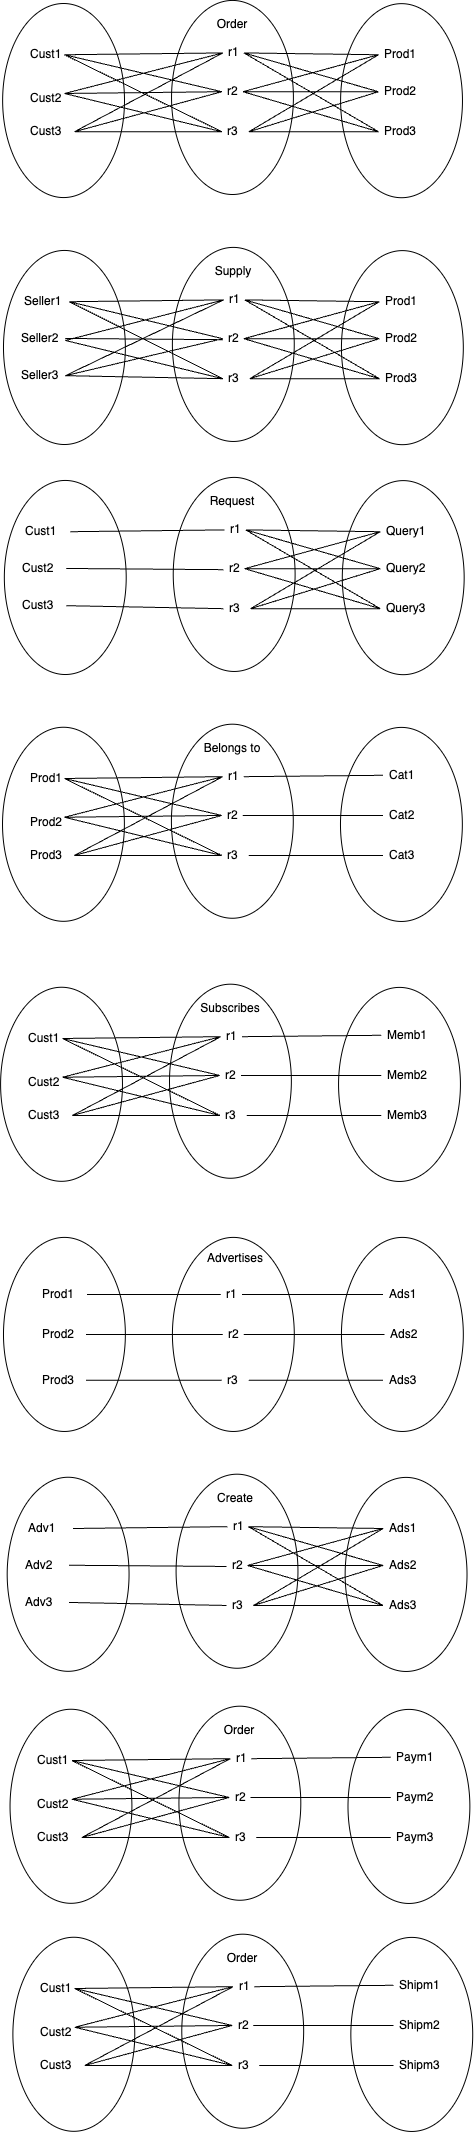
\includegraphics[width=4.79167in,height=\textheight]{relationship_set.png}

\textbf{Figure 1. Relationship Sets}

The relationship of all entities and its attributes is illustrated in
the Figure 2 of the Entity Relationship Diagram (ERD)

\textbf{Figure 2. Entity Relationship Diagram (ERD)}

\hypertarget{logical-design}{%
\subsection{Logical Design}\label{logical-design}}

Logical design is used to translate the conceptual ERD model for the
application into normalised data requirements. The logical design of the
e-commerce database is shown in Figure 3. The primary key is indicated
using one underline while foreign key is indicated using double
underline

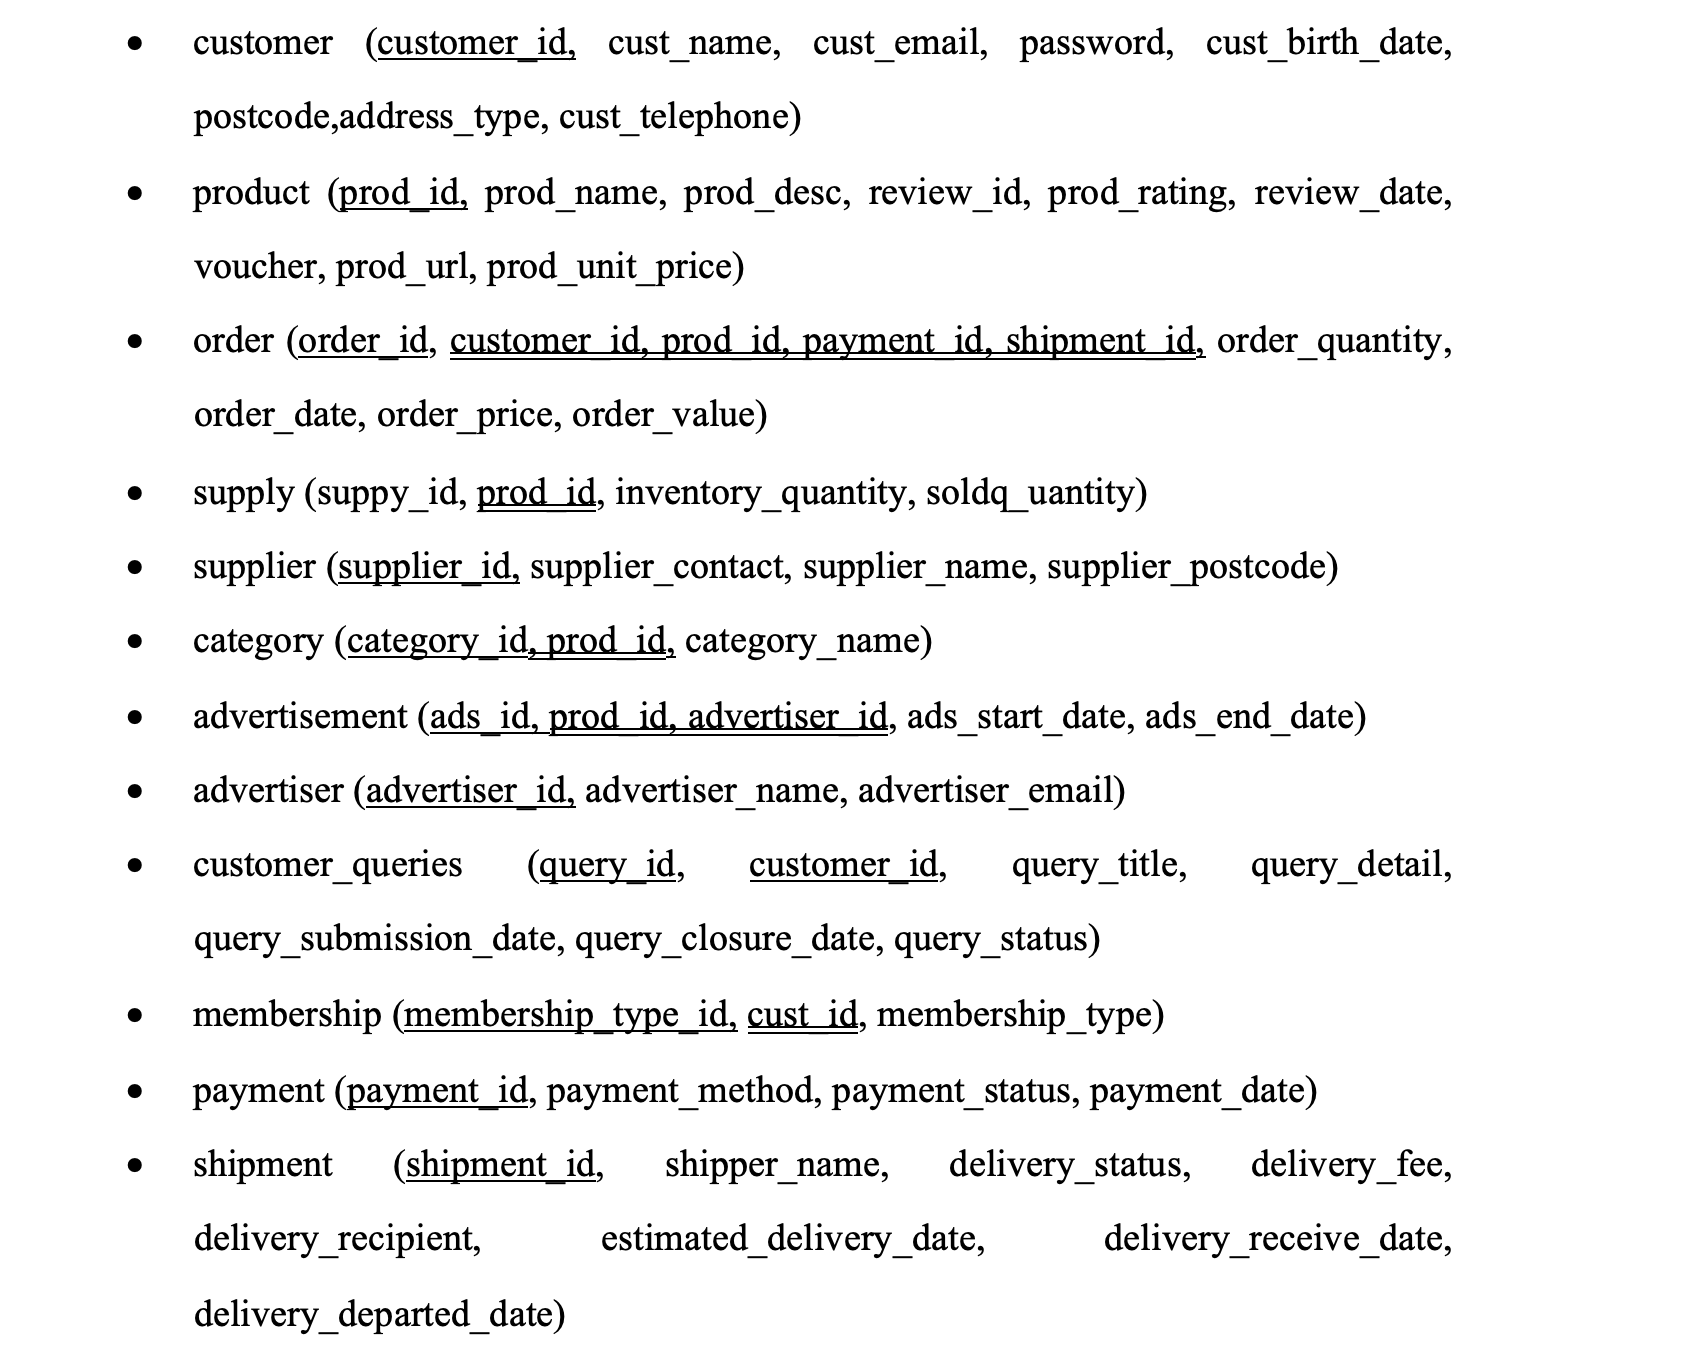
\includegraphics[width=6.41667in,height=\textheight]{images/Screenshot 2024-03-18 at 17.44.13.png}

\textbf{Figure 3. Logical Schema}

\hypertarget{physical-design}{%
\subsection{Physical Design}\label{physical-design}}

The physical design refers to the implementation of the logical schema
on the physical storage devices of a Database Management System (DBMS).
For this project, SQL is used for managing and manipulating database
within a DBMS.

In this step, the data type of each attributes will be defined. The
decision regarding the data types are made based on various factors such
as the nature of the data and the volume of the data. Choosing
appropriate data types ensures data integrity, efficient storage
utilization, and optimized query performance.

\begin{Shaded}
\begin{Highlighting}[numbers=left,,]
\NormalTok{db\_file }\OtherTok{\textless{}{-}} \StringTok{"IB9HP0\_9.db"}

\CommentTok{\# Check if the database file exists and remove it}
\ControlFlowTok{if}\NormalTok{ (}\FunctionTok{file.exists}\NormalTok{(db\_file)) \{}
  \FunctionTok{file.remove}\NormalTok{(db\_file)}
\NormalTok{\}}

\CommentTok{\# Create connection to SQL database}
\NormalTok{db\_connection }\OtherTok{\textless{}{-}}\NormalTok{ RSQLite}\SpecialCharTok{::}\FunctionTok{dbConnect}\NormalTok{(RSQLite}\SpecialCharTok{::}\FunctionTok{SQLite}\NormalTok{(),}\StringTok{"IB9HP0\_9.db"}\NormalTok{)}

\CommentTok{\# Create table for products}
\FunctionTok{dbExecute}\NormalTok{(db\_connection, }
          \StringTok{"CREATE TABLE IF NOT EXISTS products (}
\StringTok{              prod\_id VARCHAR (50) PRIMARY KEY,}
\StringTok{              prod\_name VARCHAR (50) NOT NULL,}
\StringTok{              prod\_desc VARCHAR (100) NOT NULL,}
\StringTok{              voucher VARCHAR (50),}
\StringTok{              prod\_url VARCHAR (250) NOT NULL,}
\StringTok{              prod\_unit\_price DECIMAL NOT NULL}
\StringTok{              )"}
\NormalTok{          )}

\CommentTok{\#Create table for reviews}
\FunctionTok{dbExecute}\NormalTok{(db\_connection, }
          \StringTok{"CREATE TABLE IF NOT EXISTS reviews (}
\StringTok{              review\_id VARCHAR (50) PRIMARY KEY,}
\StringTok{              prod\_rating DECIMAL NOT NULL,}
\StringTok{              review\_date DATE NOT NULL,}
\StringTok{              prod\_id VARCHAR (50),}
\StringTok{              FOREIGN KEY (prod\_id)}
\StringTok{              REFERENCES products(prod\_id)}
\StringTok{              )"}
\NormalTok{          )}

\CommentTok{\#Create table for memberships}
\FunctionTok{dbExecute}\NormalTok{(db\_connection, }
          \StringTok{"CREATE TABLE IF NOT EXISTS memberships (}
\StringTok{              membership\_type\_id VARCHAR (50) PRIMARY KEY,}
\StringTok{              membership\_type VARCHAR (50) NOT NULL}
\StringTok{              )"}
\NormalTok{          )}

\CommentTok{\#Create table for customers}
\FunctionTok{dbExecute}\NormalTok{(db\_connection, }
          \StringTok{"CREATE TABLE IF NOT EXISTS customers (}
\StringTok{              cust\_id VARCHAR (50) PRIMARY KEY,}
\StringTok{              first\_name VARCHAR (50) NOT NULL,}
\StringTok{              last\_name VARCHAR (50),}
\StringTok{              cust\_email VARCHAR (50) UNIQUE,}
\StringTok{              password VARCHAR (50) NOT NULL,}
\StringTok{              cust\_birth\_date DATE,}
\StringTok{              address\_type VARCHAR (50),}
\StringTok{              block\_num VARCHAR (50),}
\StringTok{              postcode VARCHAR (50),}
\StringTok{              cust\_telephone INT UNIQUE,}
\StringTok{              membership\_type\_id VARCHAR (50),}
\StringTok{              FOREIGN KEY (membership\_type\_id)}
\StringTok{                REFERENCES memberships(membership\_type\_id)}
\StringTok{              )"}
\NormalTok{          )}

\CommentTok{\#Create table for orders}
\FunctionTok{dbExecute}\NormalTok{(db\_connection, }
          \StringTok{"CREATE TABLE IF NOT EXISTS orders (}
\StringTok{              order\_id VARCHAR (50) PRIMARY KEY,}
\StringTok{              cust\_id VARCHAR (50),}
\StringTok{              FOREIGN KEY (cust\_id)}
\StringTok{                REFERENCES customers(cust\_id)}
\StringTok{              )"}
\NormalTok{          )}

\CommentTok{\#Create table for order details}
\FunctionTok{dbExecute}\NormalTok{(db\_connection, }
          \StringTok{"CREATE TABLE IF NOT EXISTS order\_details (}
\StringTok{              order\_quantity INT NOT NULL,}
\StringTok{              order\_date DATE,}
\StringTok{              order\_price DECIMAL NOT NULL,}
\StringTok{              order\_value DECIMAL,}
\StringTok{              prod\_id VARCHAR (50),}
\StringTok{              order\_id VARCHAR (50),}
\StringTok{              FOREIGN KEY (prod\_id)}
\StringTok{                REFERENCES products(prod\_id),}
\StringTok{              FOREIGN KEY (order\_id)}
\StringTok{                REFERENCES orders(order\_id)}
\StringTok{              )"}
\NormalTok{          )}

\CommentTok{\#Create table for payment}
\FunctionTok{dbExecute}\NormalTok{(db\_connection, }
          \StringTok{"CREATE TABLE IF NOT EXISTS payments (}
\StringTok{              payment\_id VARCHAR (50) PRIMARY KEY,}
\StringTok{              payment\_method VARCHAR (100) NOT NULL,}
\StringTok{              payment\_amount DECIMAL,}
\StringTok{              payment\_status VARCHAR (100) NOT NULL,}
\StringTok{              payment\_date DATE,}
\StringTok{              order\_id VARCHAR (50),}
\StringTok{              FOREIGN KEY (order\_id)}
\StringTok{                REFERENCES orders(order\_id)}
\StringTok{              )"}
\NormalTok{          )}

\CommentTok{\#Create table for shipment}
\FunctionTok{dbExecute}\NormalTok{(db\_connection, }
          \StringTok{"CREATE TABLE IF NOT EXISTS shipments (}
\StringTok{              shipment\_id VARCHAR (50) PRIMARY KEY,}
\StringTok{              delivery\_status VARCHAR (50),}
\StringTok{              delivery\_fee DECIMAL,}
\StringTok{              delivery\_recipient VARCHAR (50),}
\StringTok{              shipper\_name VARCHAR (50),}
\StringTok{              est\_delivery\_date DATE,}
\StringTok{              delivery\_departed\_date DATE,}
\StringTok{              delivery\_received\_date DATE,}
\StringTok{              prod\_id VARCHAR (50),}
\StringTok{              order\_id VARCHAR (50),}
\StringTok{              FOREIGN KEY (prod\_id)}
\StringTok{                REFERENCES products(prod\_id),}
\StringTok{              FOREIGN KEY (order\_id)}
\StringTok{                REFERENCES orders(order\_id)}
\StringTok{            )"}
\NormalTok{          )}

\CommentTok{\#Create table for supplier}
\FunctionTok{dbExecute}\NormalTok{(db\_connection, }
          \StringTok{"CREATE TABLE IF NOT EXISTS suppliers (}
\StringTok{              supplier\_id VARCHAR (50) PRIMARY KEY,}
\StringTok{              supplier\_name VARCHAR (50) NOT NULL UNIQUE,}
\StringTok{              supplier\_postcode VARCHAR (100) NOT NULL UNIQUE,}
\StringTok{              supplier\_contact INT NOT NULL UNIQUE}
\StringTok{            )"}
\NormalTok{          )}

\CommentTok{\#Create table for supplies}
\FunctionTok{dbExecute}\NormalTok{(db\_connection, }
          \StringTok{"CREATE TABLE IF NOT EXISTS supplies (}
\StringTok{              supply\_id VARCHAR (50) PRIMARY KEY,}
\StringTok{              inventory\_quantity INT NOT NULL,}
\StringTok{              sold\_quantity INT NOT NULL,}
\StringTok{              supplier\_id VARCHAR (50),}
\StringTok{              prod\_id VARCHAR (50),}
\StringTok{              FOREIGN KEY (supplier\_id)}
\StringTok{                REFERENCES suppliers(supplier\_id),}
\StringTok{              FOREIGN KEY (prod\_id)}
\StringTok{                REFERENCES products(prod\_id)}
\StringTok{            )"}
\NormalTok{          )}

\CommentTok{\#Create table for customer queries}
\FunctionTok{dbExecute}\NormalTok{(db\_connection, }
          \StringTok{"CREATE TABLE IF NOT EXISTS customer\_queries (}
\StringTok{              query\_id VARCHAR (50) PRIMARY KEY,}
\StringTok{              query\_title VARCHAR (50) NOT NULL,}
\StringTok{              query\_submission\_date DATE,}
\StringTok{              query\_closure\_date DATE,}
\StringTok{              query\_status VARCHAR (50) NOT NULL,}
\StringTok{              cust\_id VARCHAR (50),}
\StringTok{              FOREIGN KEY (cust\_id)}
\StringTok{                REFERENCES customers(cust\_id)}
\StringTok{            )"}
\NormalTok{          )}

\CommentTok{\#Create table for categories}
\FunctionTok{dbExecute}\NormalTok{(db\_connection, }
          \StringTok{"CREATE TABLE IF NOT EXISTS categories (}
\StringTok{              category\_id VARCHAR (50) PRIMARY KEY,}
\StringTok{              category\_name VARCHAR (50) NOT NULL UNIQUE}
\StringTok{            )"}
\NormalTok{          )}

\CommentTok{\#Create table for product categories}
\FunctionTok{dbExecute}\NormalTok{(db\_connection, }
          \StringTok{"CREATE TABLE IF NOT EXISTS product\_categories (}
\StringTok{              category\_id VARCHAR (50),}
\StringTok{              prod\_id VARCHAR (50),}
\StringTok{              FOREIGN KEY (prod\_id)}
\StringTok{                REFERENCES categories(category\_id),}
\StringTok{              FOREIGN KEY (prod\_id)}
\StringTok{                REFERENCES products(prod\_id)}
\StringTok{            )"}
\NormalTok{          )}

\CommentTok{\#Create table for advertiser}
\FunctionTok{dbExecute}\NormalTok{(db\_connection, }
          \StringTok{"CREATE TABLE IF NOT EXISTS advertisers (}
\StringTok{              advertiser\_id VARCHAR (50) PRIMARY KEY,}
\StringTok{              advertiser\_name VARCHAR (50) NOT NULL UNIQUE,}
\StringTok{              advertiser\_email VARCHAR (50) UNIQUE}
\StringTok{            )"}
\NormalTok{          )}

\CommentTok{\#Create table for advertisements}
\FunctionTok{dbExecute}\NormalTok{(db\_connection, }
          \StringTok{"CREATE TABLE IF NOT EXISTS advertisements (}
\StringTok{              ads\_id VARCHAR (50) PRIMARY KEY,}
\StringTok{              ads\_start\_date DATE,}
\StringTok{              ads\_end\_date DATE,}
\StringTok{              prod\_id VARCHAR (50) UNIQUE,}
\StringTok{              advertiser\_id VARCHAR (50),}
\StringTok{              FOREIGN KEY (prod\_id)}
\StringTok{                REFERENCES products(prod\_id),}
\StringTok{              FOREIGN KEY (advertiser\_id)}
\StringTok{                REFERENCES advertisers(advertiser\_id)  }
\StringTok{            )"}
\NormalTok{          )}
\end{Highlighting}
\end{Shaded}

\hypertarget{data-generation-and-management}{%
\section{Data Generation and
Management}\label{data-generation-and-management}}

\hypertarget{synthethic-data-generation}{%
\subsection{Synthethic Data
Generation}\label{synthethic-data-generation}}

The data used in the project is generated using R using several packages
including randomNames, dplyr, tidyr, chartlatan, stringi, lubridate, and
conjurer. Additionally, AI is used to generate names, categories, and
descriptions. For the address, the postcode referred to the data
provided by Office for National Statistics (ONS)

\begin{Shaded}
\begin{Highlighting}[numbers=left,,]
\DocumentationTok{\#\# Synthetic Data Generation \#1}

\DocumentationTok{\#\#\# \textquotesingle{}customers\textquotesingle{} table}
\CommentTok{\#Define parameters for customers}
\FunctionTok{set.seed}\NormalTok{(}\DecValTok{312}\NormalTok{)}
\NormalTok{n\_customers }\OtherTok{\textless{}{-}} \DecValTok{100}
\NormalTok{birthdate }\OtherTok{\textless{}{-}} \FunctionTok{sample}\NormalTok{(}\FunctionTok{seq}\NormalTok{(}\AttributeTok{from =} \FunctionTok{as.Date}\NormalTok{(}\FunctionTok{today}\NormalTok{() }\SpecialCharTok{{-}} \FunctionTok{years}\NormalTok{(}\DecValTok{80}\NormalTok{), }\StringTok{"\%d{-}\%m{-}\%Y"}\NormalTok{), }
                        \AttributeTok{to =} \FunctionTok{as.Date}\NormalTok{(}\FunctionTok{today}\NormalTok{() }\SpecialCharTok{{-}} \FunctionTok{years}\NormalTok{(}\DecValTok{18}\NormalTok{), }\StringTok{"\%d{-}\%m{-}\%Y"}\NormalTok{), }\AttributeTok{by =} \StringTok{"day"}\NormalTok{),}
\NormalTok{                    n\_customers)}
\NormalTok{cv\_postcode }\OtherTok{\textless{}{-}} 
  \FunctionTok{read.csv}\NormalTok{(}\StringTok{"data\_uploads/ONSPD\_AUG\_2023\_UK\_CV.csv"}\NormalTok{)[, }\DecValTok{1}\NormalTok{] }\SpecialCharTok{\%\textgreater{}\%} 
  \FunctionTok{data.frame}\NormalTok{() }\SpecialCharTok{\%\textgreater{}\%} 
  \FunctionTok{setNames}\NormalTok{(}\StringTok{"pcd"}\NormalTok{)}
\NormalTok{address\_type }\OtherTok{\textless{}{-}} \FunctionTok{c}\NormalTok{(}\StringTok{"Home"}\NormalTok{, }\StringTok{"Office"}\NormalTok{)}
\CommentTok{\#Create data}
\NormalTok{customers\_data }\OtherTok{\textless{}{-}} 
  \CommentTok{\#Create n unique customer IDs with random names}
  \FunctionTok{data.frame}\NormalTok{(}\StringTok{"cust\_id"} \OtherTok{=}\NormalTok{ conjurer}\SpecialCharTok{::}\FunctionTok{buildCust}\NormalTok{(n\_customers),}
             \StringTok{"cust\_name"} \OtherTok{=}\NormalTok{ randomNames}\SpecialCharTok{::}\FunctionTok{randomNames}\NormalTok{(n\_customers)) }\SpecialCharTok{\%\textgreater{}\%} 
  \FunctionTok{separate}\NormalTok{(cust\_name, }\AttributeTok{into =} \FunctionTok{c}\NormalTok{(}\StringTok{"last\_name"}\NormalTok{, }\StringTok{"first\_name"}\NormalTok{), }\AttributeTok{sep =} \StringTok{", "}\NormalTok{) }\SpecialCharTok{\%\textgreater{}\%}
  \CommentTok{\#Create email column, by merging last \& first name with email domain @gmail.com}
  \FunctionTok{unite}\NormalTok{(cust\_email, }\FunctionTok{c}\NormalTok{(last\_name, first\_name), }\AttributeTok{sep =} \StringTok{"."}\NormalTok{, }\AttributeTok{remove =}\NormalTok{ F) }\SpecialCharTok{\%\textgreater{}\%}
  \FunctionTok{mutate}\NormalTok{(}
    \StringTok{"cust\_email"} \OtherTok{=} \FunctionTok{paste}\NormalTok{(cust\_email,}\StringTok{"gmail.com"}\NormalTok{, }\AttributeTok{sep =} \StringTok{"@"}\NormalTok{),}
    \CommentTok{\#Generate user\textquotesingle{}s password, using random string generation package}
    \StringTok{"password"} \OtherTok{=} 
\NormalTok{      stringi}\SpecialCharTok{::}\FunctionTok{stri\_rand\_strings}\NormalTok{(}\AttributeTok{n=}\NormalTok{n\_customers, }\AttributeTok{length=}\DecValTok{8}\NormalTok{, }\AttributeTok{pattern=}\StringTok{"[A{-}Za{-}z0{-}9]"}\NormalTok{),}
    \CommentTok{\#Adding customer BOD}
    \StringTok{"cust\_birth\_date"} \OtherTok{=} \FunctionTok{sample}\NormalTok{(birthdate, n\_customers, }\AttributeTok{replace =}\NormalTok{ T),}
    \CommentTok{\#Adding the phone code in UK}
    \StringTok{"phone\_domain"} \OtherTok{=} \StringTok{"075"}\NormalTok{,}
    \CommentTok{\#create unique random strings of 7 digits}
    \StringTok{"cust\_telephone"} \OtherTok{=} 
\NormalTok{      stringi}\SpecialCharTok{::}\FunctionTok{stri\_rand\_strings}\NormalTok{(}\AttributeTok{n=}\NormalTok{n\_customers, }\AttributeTok{length=}\DecValTok{7}\NormalTok{, }\AttributeTok{pattern=}\StringTok{"[0{-}9]"}\NormalTok{),}
    \StringTok{"block\_num"} \OtherTok{=} 
      \FunctionTok{sprintf}\NormalTok{(}\StringTok{"\%s\%s"}\NormalTok{, }
              \FunctionTok{stri\_rand\_strings}\NormalTok{(}\AttributeTok{n=}\NormalTok{n\_customers, }\AttributeTok{length=}\DecValTok{1}\NormalTok{, }\AttributeTok{pattern=}\StringTok{"[A{-}Z]"}\NormalTok{),}
              \FunctionTok{stri\_rand\_strings}\NormalTok{(}\AttributeTok{n=}\NormalTok{n\_customers, }\AttributeTok{length=}\DecValTok{2}\NormalTok{, }\AttributeTok{pattern=}\StringTok{"[0{-}99]"}\NormalTok{)),}
    \CommentTok{\#randomly assign postcode to each customer}
    \StringTok{"postcode"} \OtherTok{=}\NormalTok{ cv\_postcode[}\FunctionTok{sample}\NormalTok{(}\FunctionTok{nrow}\NormalTok{(cv\_postcode), n\_customers),],}
    \CommentTok{\#randomly assign address type to each customer}
    \StringTok{"address\_type"} \OtherTok{=} \FunctionTok{sample}\NormalTok{(address\_type, n\_customers, }\AttributeTok{replace =}\NormalTok{ T)) }\SpecialCharTok{\%\textgreater{}\%}
  \CommentTok{\#Adding customer\textquotesingle{}s telephone number by merging two phone number columns}
  \FunctionTok{unite}\NormalTok{(cust\_telephone, }
        \FunctionTok{c}\NormalTok{(phone\_domain, cust\_telephone), }\AttributeTok{sep =} \StringTok{""}\NormalTok{, }\AttributeTok{remove =}\NormalTok{ T) }\SpecialCharTok{\%\textgreater{}\%}
  \CommentTok{\#reorder the columns}
  \FunctionTok{select}\NormalTok{(}\DecValTok{1}\NormalTok{,}\DecValTok{4}\NormalTok{,}\DecValTok{3}\NormalTok{,}\DecValTok{2}\NormalTok{,}\DecValTok{5}\NormalTok{,}\DecValTok{6}\NormalTok{,}\DecValTok{8}\NormalTok{,}\DecValTok{9}\NormalTok{,}\DecValTok{10}\NormalTok{,}\DecValTok{7}\NormalTok{)}
\NormalTok{customers\_data}\SpecialCharTok{$}\NormalTok{cust\_birth\_date }\OtherTok{\textless{}{-}} \FunctionTok{format}\NormalTok{(customers\_data}\SpecialCharTok{$}\NormalTok{cust\_birth\_date, }\StringTok{"\%d{-}\%m{-}\%Y"}\NormalTok{)}
\CommentTok{\#Save data to data file}
\FunctionTok{write.csv}\NormalTok{(customers\_data, }\StringTok{"data\_uploads/R\_synth\_customers\_round1.csv"}\NormalTok{)}

\DocumentationTok{\#\#\# \textquotesingle{}products\textquotesingle{} table}
\CommentTok{\#Getting brand and product names from Gemini}
\NormalTok{gemini\_prods }\OtherTok{\textless{}{-}} 
\NormalTok{  readxl}\SpecialCharTok{::}\FunctionTok{read\_excel}\NormalTok{(}\StringTok{"data\_uploads/gemini\_prod\_cate\_supplier.xlsx"}\NormalTok{, }
                     \AttributeTok{.name\_repair =} \StringTok{"universal"}\NormalTok{) }\SpecialCharTok{\%\textgreater{}\%}
  \FunctionTok{setNames}\NormalTok{(}\FunctionTok{c}\NormalTok{(}\StringTok{"seller\_name"}\NormalTok{, }\StringTok{"category"}\NormalTok{, }\StringTok{"prod\_name"}\NormalTok{, }\StringTok{"prod\_desc"}\NormalTok{))}
\CommentTok{\#Define parameters for products}
\FunctionTok{set.seed}\NormalTok{(}\DecValTok{123}\NormalTok{)}
\NormalTok{n\_prods }\OtherTok{\textless{}{-}} \DecValTok{20}
\NormalTok{voucher\_type }\OtherTok{\textless{}{-}} \FunctionTok{c}\NormalTok{(}\StringTok{"10\%"}\NormalTok{, }\StringTok{"20\%"}\NormalTok{, }\StringTok{"50\%"}\NormalTok{)}
\NormalTok{ratings }\OtherTok{\textless{}{-}} \FunctionTok{c}\NormalTok{(}\DecValTok{1}\NormalTok{,}\DecValTok{2}\NormalTok{,}\DecValTok{3}\NormalTok{,}\DecValTok{4}\NormalTok{,}\DecValTok{5}\NormalTok{)}
\NormalTok{date }\OtherTok{\textless{}{-}} \CommentTok{\#assuming company was established on Mar 06th 2004, data here is }
  \FunctionTok{sample}\NormalTok{(}\FunctionTok{seq}\NormalTok{(}\AttributeTok{from =} \FunctionTok{as.Date}\NormalTok{(}\StringTok{"2004/03/06"}\NormalTok{), }
             \AttributeTok{to =} \FunctionTok{as.Date}\NormalTok{(lubridate}\SpecialCharTok{::}\FunctionTok{today}\NormalTok{()), }\AttributeTok{by =} \StringTok{"day"}\NormalTok{), }\DecValTok{12}\NormalTok{)}
\CommentTok{\#Assign product ID, and adding product names and URL}
\NormalTok{products\_data }\OtherTok{\textless{}{-}} 
  \CommentTok{\#generate product id}
\NormalTok{  conjurer}\SpecialCharTok{::}\FunctionTok{buildProd}\NormalTok{(n\_prods, }\AttributeTok{minPrice =} \DecValTok{1}\NormalTok{, }\AttributeTok{maxPrice =} \DecValTok{100}\NormalTok{) }\SpecialCharTok{\%\textgreater{}\%} 
  \CommentTok{\#add product name and description from gemini\textquotesingle{}s file}
  \FunctionTok{mutate}\NormalTok{(}\StringTok{"prod\_name"} \OtherTok{=} \FunctionTok{sample}\NormalTok{(gemini\_prods}\SpecialCharTok{$}\NormalTok{prod\_name, }\DecValTok{20}\NormalTok{)) }\SpecialCharTok{\%\textgreater{}\%}
  \FunctionTok{left\_join}\NormalTok{(}\FunctionTok{select}\NormalTok{(gemini\_prods, }\SpecialCharTok{{-}}\FunctionTok{c}\NormalTok{(seller\_name, category)), }
            \AttributeTok{by =} \FunctionTok{join\_by}\NormalTok{(prod\_name)) }\SpecialCharTok{\%\textgreater{}\%}
  \CommentTok{\#rename columns to fit schema}
  \FunctionTok{rename}\NormalTok{(}\AttributeTok{prod\_id =}\NormalTok{ SKU, }\AttributeTok{prod\_unit\_price =}\NormalTok{ Price) }\SpecialCharTok{\%\textgreater{}\%}
  \CommentTok{\#rename \textasciigrave{}sku\textasciigrave{} with \textasciigrave{}prod\textasciigrave{}}
  \FunctionTok{mutate}\NormalTok{(}\StringTok{"prod\_id"} \OtherTok{=} \FunctionTok{gsub}\NormalTok{(}\StringTok{"sku"}\NormalTok{, }\StringTok{"prod"}\NormalTok{, prod\_id)) }\SpecialCharTok{\%\textgreater{}\%}
  \CommentTok{\#add product url}
  \FunctionTok{mutate}\NormalTok{(}\StringTok{"web\_prefix"} \OtherTok{=} \StringTok{"https://group9.co.uk/"}\NormalTok{,}
         \StringTok{"prod\_url1"} \OtherTok{=} \FunctionTok{gsub}\NormalTok{(}\StringTok{" "}\NormalTok{, }\StringTok{"{-}"}\NormalTok{, prod\_name)) }\SpecialCharTok{\%\textgreater{}\%}
  \FunctionTok{unite}\NormalTok{(prod\_url, }\FunctionTok{c}\NormalTok{(prod\_url1, prod\_id), }\AttributeTok{sep =} \StringTok{"{-}"}\NormalTok{, }\AttributeTok{remove =}\NormalTok{ F) }\SpecialCharTok{\%\textgreater{}\%}
  \FunctionTok{unite}\NormalTok{(prod\_url, }\FunctionTok{c}\NormalTok{(web\_prefix, prod\_url), }\AttributeTok{sep =} \StringTok{""}\NormalTok{, }\AttributeTok{remove =}\NormalTok{ T) }\SpecialCharTok{\%\textgreater{}\%}
  \FunctionTok{mutate}\NormalTok{(}
    \CommentTok{\#Create ratings}
    \StringTok{"prod\_rating"} \OtherTok{=} \FunctionTok{sample}\NormalTok{(ratings, n\_prods, }\AttributeTok{replace =}\NormalTok{ T),}
    \CommentTok{\#Review date}
    \StringTok{"review\_date"} \OtherTok{=} \FunctionTok{sample}\NormalTok{(}\FunctionTok{format}\NormalTok{(date, }\StringTok{"\%d{-}\%m{-}\%Y"}\NormalTok{), n\_prods, }\AttributeTok{replace =}\NormalTok{ T),}
    \CommentTok{\#Assign review ID}
    \StringTok{"review\_id"} \OtherTok{=} 
\NormalTok{      conjurer}\SpecialCharTok{::}\FunctionTok{buildCust}\NormalTok{(}\FunctionTok{sum}\NormalTok{(}\SpecialCharTok{!}\FunctionTok{is.na}\NormalTok{(prod\_rating))),}
    \StringTok{"review\_id"} \OtherTok{=} \FunctionTok{gsub}\NormalTok{(}\StringTok{"cust"}\NormalTok{, }\StringTok{"rev"}\NormalTok{, review\_id)) }\SpecialCharTok{\%\textgreater{}\%}
  \CommentTok{\#drop temp url}
  \FunctionTok{select}\NormalTok{(}\SpecialCharTok{{-}}\NormalTok{prod\_url1)}
\CommentTok{\#Create vouchers {-}{-} Randomly assign voucher types to 50\% of the products}
\NormalTok{voucher\_prods }\OtherTok{\textless{}{-}} \FunctionTok{sample\_n}\NormalTok{(}\FunctionTok{data.frame}\NormalTok{(products\_data}\SpecialCharTok{$}\NormalTok{prod\_id), }
                              \FloatTok{0.5}\SpecialCharTok{*}\FunctionTok{nrow}\NormalTok{(products\_data)) }\SpecialCharTok{\%\textgreater{}\%} \FunctionTok{setNames}\NormalTok{(}\StringTok{"prod\_id"}\NormalTok{)}
\NormalTok{products\_data }\OtherTok{\textless{}{-}}\NormalTok{ products\_data }\SpecialCharTok{\%\textgreater{}\%} 
  \FunctionTok{mutate}\NormalTok{(}\AttributeTok{voucher =} \FunctionTok{ifelse}\NormalTok{(products\_data}\SpecialCharTok{$}\NormalTok{prod\_id }\SpecialCharTok{\%in\%}\NormalTok{ voucher\_prods}\SpecialCharTok{$}\NormalTok{prod\_id, }
                          \FunctionTok{sample}\NormalTok{(voucher\_type, }\FunctionTok{nrow}\NormalTok{(voucher\_prods), }\AttributeTok{replace =}\NormalTok{ T), }\ConstantTok{NA}\NormalTok{))}
\CommentTok{\#Finalise the table}
\NormalTok{products\_data }\OtherTok{\textless{}{-}} 
\NormalTok{  products\_data }\SpecialCharTok{\%\textgreater{}\%}
  \CommentTok{\#rearrange order of columns}
  \FunctionTok{select}\NormalTok{(}\DecValTok{2}\NormalTok{,}\DecValTok{4}\NormalTok{,}\DecValTok{5}\NormalTok{,}\DecValTok{8}\NormalTok{,}\DecValTok{6}\NormalTok{,}\DecValTok{7}\NormalTok{,}\DecValTok{3}\NormalTok{,}\DecValTok{9}\NormalTok{,}\DecValTok{1}\NormalTok{)}
\CommentTok{\#Save to .csv file}
\FunctionTok{write.csv}\NormalTok{(products\_data, }\StringTok{"data\_uploads/R\_synth\_products\_round1.csv"}\NormalTok{)}

\DocumentationTok{\#\#\# \textquotesingle{}orders\textquotesingle{} table}
\CommentTok{\#Define parameters}
\NormalTok{origin\_date }\OtherTok{\textless{}{-}} \StringTok{"1970{-}01{-}01"}
\NormalTok{n\_orders }\OtherTok{\textless{}{-}} \DecValTok{500}
\NormalTok{order\_date }\OtherTok{\textless{}{-}} 
  \CommentTok{\#round 1 is for orders in 2022{-}Mar\textquotesingle{}2024, }
  \CommentTok{\#so all orders have been paid and delivered successfully}
  \FunctionTok{sample}\NormalTok{(}\FunctionTok{seq}\NormalTok{(}\AttributeTok{from =} \FunctionTok{as.Date}\NormalTok{(}\StringTok{"2022/01/01"}\NormalTok{), }
             \AttributeTok{to =} \FunctionTok{as.Date}\NormalTok{(}\StringTok{"2024/03/01"}\NormalTok{), }\DecValTok{12}\NormalTok{))}
\NormalTok{pymt\_method }\OtherTok{\textless{}{-}} 
  \FunctionTok{c}\NormalTok{(}\StringTok{"Bank Transfer"}\NormalTok{, }\StringTok{"Visa"}\NormalTok{, }\StringTok{"Mastercard"}\NormalTok{, }\StringTok{"PayPal"}\NormalTok{, }\StringTok{"GPay"}\NormalTok{, }\StringTok{"Apple Pay"}\NormalTok{)}
\NormalTok{pymt\_status }\OtherTok{\textless{}{-}} \FunctionTok{c}\NormalTok{(}\StringTok{"Done"}\NormalTok{, }\StringTok{"Verifying"}\NormalTok{)}
\NormalTok{shipper\_lookup }\OtherTok{\textless{}{-}} 
  \FunctionTok{data.frame}\NormalTok{(}\StringTok{"shipper\_name"} \OtherTok{=} \FunctionTok{c}\NormalTok{(}\StringTok{"DHL"}\NormalTok{, }\StringTok{"Group9DL"}\NormalTok{, }\StringTok{"DPD"}\NormalTok{),}
             \StringTok{"delivery\_fee"} \OtherTok{=} \FunctionTok{c}\NormalTok{(}\DecValTok{5}\NormalTok{,}\DecValTok{2}\NormalTok{,}\DecValTok{3}\NormalTok{),}
             \StringTok{"ETA"} \OtherTok{=} \FunctionTok{c}\NormalTok{(}\DecValTok{1}\NormalTok{,}\DecValTok{5}\NormalTok{,}\DecValTok{3}\NormalTok{))}
\NormalTok{delivery\_status }\OtherTok{\textless{}{-}} \FunctionTok{c}\NormalTok{(}\StringTok{"Delivered"}\NormalTok{, }\StringTok{"In Progress"}\NormalTok{, }
                     \StringTok{"Failed to contact"}\NormalTok{, }\StringTok{"Delayed"}\NormalTok{)}
\NormalTok{orders\_col\_order }\OtherTok{\textless{}{-}} 
  \FunctionTok{c}\NormalTok{(}\StringTok{"order\_id"}\NormalTok{, }\StringTok{"cust\_id"}\NormalTok{, }\StringTok{"prod\_id"}\NormalTok{, }\StringTok{"order\_quantity"}\NormalTok{,}
    \StringTok{"order\_date"}\NormalTok{, }\StringTok{"order\_value"}\NormalTok{, }\StringTok{"order\_price"}\NormalTok{)}
\CommentTok{\#generate n order IDs and assign customers to them, including order date}
\FunctionTok{set.seed}\NormalTok{(}\DecValTok{122}\NormalTok{)}
\NormalTok{orders\_data }\OtherTok{\textless{}{-}} 
  \CommentTok{\#Create n unique order IDs}
  \FunctionTok{data.frame}\NormalTok{(}\StringTok{"order\_id"} \OtherTok{=}\NormalTok{ conjurer}\SpecialCharTok{::}\FunctionTok{buildCust}\NormalTok{(n\_orders)) }\SpecialCharTok{\%\textgreater{}\%}
  \FunctionTok{mutate}\NormalTok{(}\AttributeTok{order\_id =} \FunctionTok{gsub}\NormalTok{(}\StringTok{"cust"}\NormalTok{, }\StringTok{"o"}\NormalTok{, order\_id),}
         \AttributeTok{payment\_id =} \FunctionTok{gsub}\NormalTok{(}\StringTok{"o"}\NormalTok{, }\StringTok{"pm"}\NormalTok{, order\_id),}
         \AttributeTok{cust\_id =} \FunctionTok{sample}\NormalTok{(customers\_data}\SpecialCharTok{$}\NormalTok{cust\_id, n\_orders, }\AttributeTok{replace =}\NormalTok{ T),}
         \AttributeTok{order\_date =} \FunctionTok{sample}\NormalTok{(order\_date, n\_orders, }\AttributeTok{replace =}\NormalTok{ T),}
         \AttributeTok{payment\_method =} \FunctionTok{sample}\NormalTok{(pymt\_method, n\_orders, }\AttributeTok{replace =}\NormalTok{ T),}
         \AttributeTok{payment\_status =} \StringTok{"Done"}\NormalTok{,}
         \AttributeTok{delivery\_recipient =}\NormalTok{ randomNames}\SpecialCharTok{::}\FunctionTok{randomNames}\NormalTok{(n\_orders,}
                                                       \AttributeTok{which.names =} \StringTok{"first"}\NormalTok{))}
\CommentTok{\#adding payment date with logic dependent on payment status}
\NormalTok{orders\_data }\OtherTok{\textless{}{-}}\NormalTok{ orders\_data }\SpecialCharTok{\%\textgreater{}\%}
  \FunctionTok{mutate}\NormalTok{(}\StringTok{"payment\_date"} \OtherTok{=} \FunctionTok{ifelse}\NormalTok{(payment\_status }\SpecialCharTok{==} \StringTok{"Done"}\NormalTok{, order\_date, }\ConstantTok{NA}\NormalTok{)) }\SpecialCharTok{\%\textgreater{}\%}
  \FunctionTok{mutate}\NormalTok{(}\StringTok{"payment\_date"} \OtherTok{=} \FunctionTok{as.Date}\NormalTok{(payment\_date, }
                                  \AttributeTok{origin =}\NormalTok{ origin\_date))}
\CommentTok{\#randomly replicate certain orders to map with products}
\FunctionTok{set.seed}\NormalTok{(}\DecValTok{122}\NormalTok{)}
\NormalTok{orders\_data }\OtherTok{\textless{}{-}}\NormalTok{ orders\_data }\SpecialCharTok{\%\textgreater{}\%} \FunctionTok{bind\_rows}\NormalTok{() }\SpecialCharTok{\%\textgreater{}\%}
  \FunctionTok{rbind}\NormalTok{(}\FunctionTok{sample\_n}\NormalTok{(orders\_data, }\FloatTok{0.4}\SpecialCharTok{*}\FunctionTok{nrow}\NormalTok{(orders\_data)),}
        \FunctionTok{sample\_n}\NormalTok{(orders\_data, }\FloatTok{0.5}\SpecialCharTok{*}\FunctionTok{nrow}\NormalTok{(orders\_data)),}
        \FunctionTok{sample\_n}\NormalTok{(orders\_data, }\FloatTok{0.8}\SpecialCharTok{*}\FunctionTok{nrow}\NormalTok{(orders\_data)))}
\CommentTok{\#assign products to orders}
\NormalTok{orders\_data }\OtherTok{\textless{}{-}}\NormalTok{ orders\_data }\SpecialCharTok{\%\textgreater{}\%}
  \FunctionTok{mutate}\NormalTok{(}
    \StringTok{"prod\_id"} \OtherTok{=} \FunctionTok{sample}\NormalTok{(products\_data}\SpecialCharTok{$}\NormalTok{prod\_id, }
                       \FunctionTok{nrow}\NormalTok{(orders\_data), }\AttributeTok{replace =}\NormalTok{ T),}
    \CommentTok{\#generate order quantity}
    \StringTok{"order\_quantity"} \OtherTok{=} \FunctionTok{sample}\NormalTok{(}\FunctionTok{seq}\NormalTok{(}\DecValTok{1}\NormalTok{,}\DecValTok{10}\NormalTok{,}\DecValTok{1}\NormalTok{), }\FunctionTok{nrow}\NormalTok{(orders\_data), }\AttributeTok{replace =}\NormalTok{ T)) }\SpecialCharTok{\%\textgreater{}\%}
  \FunctionTok{merge}\NormalTok{(}\FunctionTok{select}\NormalTok{(products\_data, }\FunctionTok{c}\NormalTok{(prod\_id, prod\_unit\_price, voucher)), }
        \AttributeTok{by =} \StringTok{"prod\_id"}\NormalTok{)}
\CommentTok{\#Order value and shipper}
\NormalTok{orders\_data }\OtherTok{\textless{}{-}}\NormalTok{ orders\_data }\SpecialCharTok{\%\textgreater{}\%}
  \CommentTok{\#order price and value}
  \FunctionTok{mutate}\NormalTok{(}
    \AttributeTok{voucher =} \FunctionTok{as.numeric}\NormalTok{(}\FunctionTok{gsub}\NormalTok{(}\StringTok{"\%"}\NormalTok{, }\StringTok{""}\NormalTok{, voucher))}\SpecialCharTok{/}\DecValTok{100}\NormalTok{,}
    \CommentTok{\#product unit price is discounted in case of voucher available}
    \AttributeTok{order\_price =} \FunctionTok{ifelse}\NormalTok{(}\SpecialCharTok{!}\FunctionTok{is.na}\NormalTok{(voucher), }
\NormalTok{                         prod\_unit\_price }\SpecialCharTok{*}\NormalTok{ voucher, prod\_unit\_price),}
    \AttributeTok{order\_value =}\NormalTok{ order\_price }\SpecialCharTok{*}\NormalTok{ order\_quantity,}
    \CommentTok{\#assign shippers to products}
    \AttributeTok{shipper\_name =} 
      \FunctionTok{sample}\NormalTok{(shipper\_lookup}\SpecialCharTok{$}\NormalTok{shipper\_name, }\FunctionTok{nrow}\NormalTok{(orders\_data), }\AttributeTok{replace =}\NormalTok{ T),}
    \CommentTok{\#add delivery status}
    \AttributeTok{delivery\_status =} \StringTok{"Delivered"}\NormalTok{ ) }\SpecialCharTok{\%\textgreater{}\%}
  \CommentTok{\#lookup delivery fee}
  \FunctionTok{merge}\NormalTok{(shipper\_lookup, }\AttributeTok{by =} \StringTok{"shipper\_name"}\NormalTok{)}
\CommentTok{\#dates of delivery}
\NormalTok{orders\_data }\OtherTok{\textless{}{-}}\NormalTok{ orders\_data }\SpecialCharTok{\%\textgreater{}\%}
  \CommentTok{\#departure and ETA}
  \FunctionTok{mutate}\NormalTok{(}
    \AttributeTok{delivery\_departed\_date =} 
      \FunctionTok{ifelse}\NormalTok{(}\SpecialCharTok{!}\FunctionTok{is.na}\NormalTok{(payment\_date), (payment\_date }\SpecialCharTok{+} \FunctionTok{days}\NormalTok{(}\DecValTok{2}\NormalTok{)), }\ConstantTok{NA}\NormalTok{),}
    \AttributeTok{est\_delivery\_date =}\NormalTok{ delivery\_departed\_date }\SpecialCharTok{+}\NormalTok{ ETA) }\SpecialCharTok{\%\textgreater{}\%}
  \CommentTok{\#departure and ETA {-} format as date}
  \FunctionTok{mutate}\NormalTok{(}
    \AttributeTok{delivery\_departed\_date =} 
      \FunctionTok{as.Date}\NormalTok{(delivery\_departed\_date, }\AttributeTok{origin =}\NormalTok{ origin\_date),}
    \AttributeTok{est\_delivery\_date =} 
      \FunctionTok{as.Date}\NormalTok{(est\_delivery\_date, }\AttributeTok{origin =}\NormalTok{ origin\_date)) }\SpecialCharTok{\%\textgreater{}\%}
  \CommentTok{\#received}
  \FunctionTok{mutate}\NormalTok{(}
    \AttributeTok{delivery\_received\_date =} 
      \FunctionTok{ifelse}\NormalTok{(delivery\_status }\SpecialCharTok{!=} \StringTok{"Delivered"}\NormalTok{, }\ConstantTok{NA}\NormalTok{, est\_delivery\_date)) }\SpecialCharTok{\%\textgreater{}\%}
  \FunctionTok{mutate}\NormalTok{(}
    \AttributeTok{delivery\_received\_date =} 
      \FunctionTok{as.Date}\NormalTok{(delivery\_received\_date, }\AttributeTok{origin =}\NormalTok{ origin\_date)) }\SpecialCharTok{\%\textgreater{}\%}
  \CommentTok{\#drop ETA}
  \FunctionTok{select}\NormalTok{(}\SpecialCharTok{{-}}\NormalTok{ETA)}

\DocumentationTok{\#\#\# generate \textquotesingle{}shipment\textquotesingle{} from orders}
\NormalTok{shipment\_colnames }\OtherTok{\textless{}{-}} \FunctionTok{c}\NormalTok{(}\StringTok{"order\_id"}\NormalTok{, }\StringTok{"prod\_id"}\NormalTok{, }
                       \StringTok{"delivery\_departed\_date"}\NormalTok{,}
                       \StringTok{"delivery\_received\_date"}\NormalTok{, }\StringTok{"est\_delivery\_date"}\NormalTok{,}
                       \StringTok{"shipper\_name"}\NormalTok{, }\StringTok{"delivery\_recipient"}\NormalTok{,}
                       \StringTok{"delivery\_fee"}\NormalTok{, }\StringTok{"delivery\_status"}\NormalTok{)}
\NormalTok{shipment\_data }\OtherTok{\textless{}{-}} \FunctionTok{select}\NormalTok{(orders\_data, shipment\_colnames)}
\NormalTok{shipment\_data }\OtherTok{\textless{}{-}}\NormalTok{ shipment\_data }\SpecialCharTok{\%\textgreater{}\%} 
  \FunctionTok{mutate}\NormalTok{(}\AttributeTok{shipment\_id =} \FunctionTok{paste}\NormalTok{(}\StringTok{"sm"}\NormalTok{, }\FunctionTok{rownames}\NormalTok{(shipment\_data), }\AttributeTok{sep =} \StringTok{""}\NormalTok{), }
         \AttributeTok{.before =} \StringTok{"order\_id"}\NormalTok{)}
\CommentTok{\#reformat date}
\NormalTok{shipment\_dates }\OtherTok{\textless{}{-}} \FunctionTok{c}\NormalTok{(}\StringTok{"delivery\_departed\_date"}\NormalTok{,}
                    \StringTok{"delivery\_received\_date"}\NormalTok{, }\StringTok{"est\_delivery\_date"}\NormalTok{)}
\NormalTok{shipment\_data[shipment\_dates] }\OtherTok{\textless{}{-}} \FunctionTok{lapply}\NormalTok{(shipment\_data[shipment\_dates],}
\NormalTok{                                        format, }\StringTok{"\%d{-}\%m{-}\%Y"}\NormalTok{)}
\CommentTok{\#Save data to data file}
\FunctionTok{write.csv}\NormalTok{(shipment\_data, }\StringTok{"data\_uploads/R\_synth\_shipment\_round1.csv"}\NormalTok{)}

\DocumentationTok{\#\#\# generate \textquotesingle{}payment\textquotesingle{} from orders}
\NormalTok{payment\_colnames }\OtherTok{\textless{}{-}} \FunctionTok{c}\NormalTok{(}\StringTok{"payment\_id"}\NormalTok{, }\StringTok{"payment\_method"}\NormalTok{, }\StringTok{"order\_id"}\NormalTok{,}
                      \StringTok{"payment\_status"}\NormalTok{, }\StringTok{"payment\_date"}\NormalTok{)}
\CommentTok{\#Add payment amount}
\NormalTok{payment\_data }\OtherTok{\textless{}{-}}\NormalTok{ orders\_data }\SpecialCharTok{\%\textgreater{}\%} \FunctionTok{group\_by}\NormalTok{(payment\_id) }\SpecialCharTok{\%\textgreater{}\%}
  \FunctionTok{summarise}\NormalTok{(}\AttributeTok{payment\_amount =} \FunctionTok{sum}\NormalTok{(order\_value)) }\SpecialCharTok{\%\textgreater{}\%}
  \FunctionTok{left\_join}\NormalTok{(}\FunctionTok{select}\NormalTok{(orders\_data,payment\_colnames), }\AttributeTok{by =} \StringTok{"payment\_id"}\NormalTok{)}
\CommentTok{\#remove duplicates}
\NormalTok{payment\_data }\OtherTok{\textless{}{-}} \FunctionTok{distinct}\NormalTok{(payment\_data, payment\_id, }\AttributeTok{.keep\_all =}\NormalTok{ T) }\SpecialCharTok{\%\textgreater{}\%}
  \FunctionTok{select}\NormalTok{(}\DecValTok{1}\NormalTok{,}\DecValTok{4}\NormalTok{,}\DecValTok{3}\NormalTok{,}\DecValTok{2}\NormalTok{,}\DecValTok{5}\NormalTok{,}\DecValTok{6}\NormalTok{)}
\CommentTok{\#re{-}format date}
\NormalTok{payment\_data}\SpecialCharTok{$}\NormalTok{payment\_date }\OtherTok{\textless{}{-}} \FunctionTok{format}\NormalTok{(payment\_data}\SpecialCharTok{$}\NormalTok{payment\_date, }\StringTok{"\%d{-}\%m{-}\%Y"}\NormalTok{)}
\CommentTok{\#Save data to data file}
\FunctionTok{write.csv}\NormalTok{(payment\_data, }\StringTok{"data\_uploads/R\_synth\_payment\_round1.csv"}\NormalTok{)}

\CommentTok{\#reorder the columns of \textquotesingle{}orders\textquotesingle{}}
\NormalTok{orders\_data }\OtherTok{\textless{}{-}} \FunctionTok{select}\NormalTok{(orders\_data, orders\_col\_order)}
\CommentTok{\#Save data to data file}
\FunctionTok{write.csv}\NormalTok{(orders\_data, }\StringTok{"data\_uploads/R\_synth\_orders\_round1.csv"}\NormalTok{)}

\DocumentationTok{\#\#\# \textquotesingle{}suppliers\textquotesingle{} table}
\CommentTok{\#Define parameters for suppliers table}
\FunctionTok{set.seed}\NormalTok{(}\DecValTok{123}\NormalTok{)}
\NormalTok{n\_suppliers }\OtherTok{\textless{}{-}} \FunctionTok{length}\NormalTok{(}\FunctionTok{unique}\NormalTok{(gemini\_prods}\SpecialCharTok{$}\NormalTok{seller\_name))}
\NormalTok{wc\_postcode }\OtherTok{\textless{}{-}} \FunctionTok{read.csv}\NormalTok{(}\StringTok{"data\_uploads/ONSPD\_AUG\_2023\_UK\_WC.csv"}\NormalTok{)[,}\DecValTok{1}\NormalTok{]}

\CommentTok{\#Create suppliers table}
\NormalTok{suppliers\_data }\OtherTok{\textless{}{-}} 
  \CommentTok{\#Pull seller name from gemini file}
  \FunctionTok{distinct}\NormalTok{(}\FunctionTok{select}\NormalTok{(gemini\_prods, seller\_name)) }\SpecialCharTok{\%\textgreater{}\%}
  \FunctionTok{rename}\NormalTok{(}\StringTok{"supplier\_name"} \OtherTok{=} \StringTok{"seller\_name"}\NormalTok{) }\SpecialCharTok{\%\textgreater{}\%}
  \FunctionTok{mutate}\NormalTok{(}\StringTok{"supplier\_id"} \OtherTok{=} \FunctionTok{seq}\NormalTok{(}\DecValTok{1}\NormalTok{, n\_suppliers,}\DecValTok{1}\NormalTok{),}
         \StringTok{"prefix"} \OtherTok{=} \StringTok{"s"}\NormalTok{) }\SpecialCharTok{\%\textgreater{}\%}
  \FunctionTok{unite}\NormalTok{(supplier\_id, }\FunctionTok{c}\NormalTok{(prefix, supplier\_id), }\AttributeTok{sep =} \StringTok{""}\NormalTok{, }\AttributeTok{remove =}\NormalTok{ T) }\SpecialCharTok{\%\textgreater{}\%}
  \FunctionTok{mutate}\NormalTok{(}
    \StringTok{"supplier\_postcode"} \OtherTok{=}
      \FunctionTok{sample}\NormalTok{(wc\_postcode, n\_suppliers, }\AttributeTok{replace =}\NormalTok{ T),}
    \CommentTok{\#Adding the phone code in UK}
    \StringTok{"phone\_domain"} \OtherTok{=} \StringTok{"079"}\NormalTok{,}
    \CommentTok{\#create unique random strings of 7 digits}
    \StringTok{"supplier\_contact"} \OtherTok{=} 
\NormalTok{      stringi}\SpecialCharTok{::}\FunctionTok{stri\_rand\_strings}\NormalTok{(}\AttributeTok{n=}\NormalTok{n\_suppliers, }\AttributeTok{length=}\DecValTok{7}\NormalTok{, }\AttributeTok{pattern=}\StringTok{"[0{-}9]"}\NormalTok{)) }\SpecialCharTok{\%\textgreater{}\%}
  \CommentTok{\#Adding supplier\textquotesingle{}s telephone number by merging two phone number columns}
  \FunctionTok{unite}\NormalTok{(supplier\_contact, }
        \FunctionTok{c}\NormalTok{(phone\_domain, supplier\_contact), }\AttributeTok{sep =} \StringTok{""}\NormalTok{, }\AttributeTok{remove =}\NormalTok{ T) }\SpecialCharTok{\%\textgreater{}\%}
  \FunctionTok{select}\NormalTok{(}\DecValTok{2}\NormalTok{,}\DecValTok{1}\NormalTok{,}\DecValTok{4}\NormalTok{,}\DecValTok{3}\NormalTok{)}
\CommentTok{\#Save data to data file}
\FunctionTok{write.csv}\NormalTok{(suppliers\_data, }\StringTok{"data\_uploads/R\_synth\_suppliers\_round1.csv"}\NormalTok{)}

\DocumentationTok{\#\#\# \textquotesingle{}supply\textquotesingle{} table}
\CommentTok{\#Define parameters for supply table}
\FunctionTok{set.seed}\NormalTok{(}\DecValTok{123}\NormalTok{)}
\NormalTok{order\_quant\_by\_prod }\OtherTok{\textless{}{-}}\NormalTok{ orders\_data }\SpecialCharTok{\%\textgreater{}\%}
  \FunctionTok{group\_by}\NormalTok{(prod\_id) }\SpecialCharTok{\%\textgreater{}\%} \FunctionTok{summarise}\NormalTok{(}\AttributeTok{sold\_quantity =} \FunctionTok{sum}\NormalTok{(order\_quantity))}
\NormalTok{supply\_col\_order }\OtherTok{\textless{}{-}} \FunctionTok{c}\NormalTok{(}\StringTok{"supply\_id"}\NormalTok{, }\StringTok{"supplier\_id"}\NormalTok{, }\StringTok{"prod\_id"}\NormalTok{, }
                      \StringTok{"inventory\_quantity"}\NormalTok{, }\StringTok{"sold\_quantity"}\NormalTok{)}
\CommentTok{\#Create supply table}
\NormalTok{supply\_data }\OtherTok{\textless{}{-}} \FunctionTok{select}\NormalTok{(products\_data, }\FunctionTok{c}\NormalTok{(prod\_id, prod\_name)) }\SpecialCharTok{\%\textgreater{}\%}
  \FunctionTok{merge}\NormalTok{(order\_quant\_by\_prod, }\AttributeTok{by =} \StringTok{"prod\_id"}\NormalTok{) }\SpecialCharTok{\%\textgreater{}\%}
  \FunctionTok{mutate}\NormalTok{(}\AttributeTok{sold\_quantity =} \FunctionTok{as.integer}\NormalTok{(}\FunctionTok{sample}\NormalTok{(}\FunctionTok{seq}\NormalTok{(}\FloatTok{0.2}\NormalTok{,}\DecValTok{1}\NormalTok{),}\DecValTok{1}\NormalTok{)}\SpecialCharTok{*}\NormalTok{sold\_quantity)) }\SpecialCharTok{\%\textgreater{}\%}
  \FunctionTok{mutate}\NormalTok{(}\AttributeTok{inventory\_quantity =} 
           \FunctionTok{as.integer}\NormalTok{(sold\_quantity }\SpecialCharTok{*} \FunctionTok{sample}\NormalTok{(}\FunctionTok{seq}\NormalTok{(}\FloatTok{1.1}\NormalTok{, }\FloatTok{2.3}\NormalTok{), }\DecValTok{1}\NormalTok{))) }\SpecialCharTok{\%\textgreater{}\%}
  \FunctionTok{merge}\NormalTok{(}\FunctionTok{select}\NormalTok{(gemini\_prods, }\FunctionTok{c}\NormalTok{(seller\_name, prod\_name)), }\AttributeTok{by =} \StringTok{"prod\_name"}\NormalTok{) }\SpecialCharTok{\%\textgreater{}\%}
  \FunctionTok{rename}\NormalTok{(}\StringTok{"supplier\_name"} \OtherTok{=} \StringTok{"seller\_name"}\NormalTok{) }\SpecialCharTok{\%\textgreater{}\%}
  \FunctionTok{merge}\NormalTok{(}\FunctionTok{select}\NormalTok{(suppliers\_data, }\FunctionTok{c}\NormalTok{(supplier\_id, supplier\_name)), }
        \AttributeTok{by =} \StringTok{"supplier\_name"}\NormalTok{)}
\CommentTok{\#Create competitors for M:N relationship}
\NormalTok{supply\_competitors }\OtherTok{\textless{}{-}} \FunctionTok{select}\NormalTok{(products\_data, }\FunctionTok{c}\NormalTok{(prod\_id, prod\_name)) }\SpecialCharTok{\%\textgreater{}\%}
  \FunctionTok{mutate}\NormalTok{(}\AttributeTok{supplier\_name =} 
           \FunctionTok{sample}\NormalTok{(suppliers\_data}\SpecialCharTok{$}\NormalTok{supplier\_name, n\_prods, }\AttributeTok{replace =}\NormalTok{ T)) }\SpecialCharTok{\%\textgreater{}\%}
  \FunctionTok{merge}\NormalTok{(}\FunctionTok{select}\NormalTok{(suppliers\_data, }\FunctionTok{c}\NormalTok{(supplier\_id, supplier\_name)), }
        \AttributeTok{by =} \StringTok{"supplier\_name"}\NormalTok{) }\SpecialCharTok{\%\textgreater{}\%}
  \FunctionTok{merge}\NormalTok{(order\_quant\_by\_prod, }\AttributeTok{by =} \StringTok{"prod\_id"}\NormalTok{) }\SpecialCharTok{\%\textgreater{}\%}
  \FunctionTok{mutate}\NormalTok{(}\AttributeTok{sold\_quantity =} \FunctionTok{as.integer}\NormalTok{(}\FunctionTok{sample}\NormalTok{(}\FunctionTok{seq}\NormalTok{(}\FloatTok{0.2}\NormalTok{,}\DecValTok{1}\NormalTok{),}\DecValTok{1}\NormalTok{)}\SpecialCharTok{*}\NormalTok{sold\_quantity)) }\SpecialCharTok{\%\textgreater{}\%}
  \FunctionTok{mutate}\NormalTok{(}\AttributeTok{inventory\_quantity =} 
           \FunctionTok{as.integer}\NormalTok{(sold\_quantity }\SpecialCharTok{*} \FunctionTok{sample}\NormalTok{(}\FunctionTok{seq}\NormalTok{(}\FloatTok{1.1}\NormalTok{, }\FloatTok{2.3}\NormalTok{), }\DecValTok{1}\NormalTok{))) }\SpecialCharTok{\%\textgreater{}\%}
  \FunctionTok{select}\NormalTok{(}\DecValTok{2}\NormalTok{,}\DecValTok{3}\NormalTok{,}\DecValTok{1}\NormalTok{,}\DecValTok{5}\NormalTok{,}\DecValTok{6}\NormalTok{,}\DecValTok{4}\NormalTok{)}
\CommentTok{\#Combine supply and competitors}
\NormalTok{supply\_data }\OtherTok{\textless{}{-}} 
  \FunctionTok{rbind}\NormalTok{(supply\_data, supply\_competitors) }\SpecialCharTok{\%\textgreater{}\%} 
  \FunctionTok{mutate}\NormalTok{(}\AttributeTok{supply\_id =} \FunctionTok{paste}\NormalTok{(}\StringTok{"sp"}\NormalTok{, }\FunctionTok{row\_number}\NormalTok{(), }\AttributeTok{sep =} \StringTok{""}\NormalTok{)) }\SpecialCharTok{\%\textgreater{}\%}
  \FunctionTok{select}\NormalTok{(}\SpecialCharTok{{-}}\FunctionTok{c}\NormalTok{(supplier\_name, prod\_name))}
\CommentTok{\#reorder columns}
\NormalTok{supply\_data }\OtherTok{\textless{}{-}}\NormalTok{ supply\_data[, supply\_col\_order]}
\CommentTok{\#Save data to data file}
\FunctionTok{write.csv}\NormalTok{(supply\_data, }\StringTok{"data\_uploads/R\_synth\_supply\_round1.csv"}\NormalTok{)}

\DocumentationTok{\#\#\# \textquotesingle{}memberships\textquotesingle{} table}
\NormalTok{membership\_lookup }\OtherTok{\textless{}{-}} 
  \FunctionTok{data.frame}\NormalTok{(}
    \StringTok{"membership\_type"} \OtherTok{=}  \FunctionTok{c}\NormalTok{(}\StringTok{"Student"}\NormalTok{, }\StringTok{"Trial"}\NormalTok{, }\StringTok{"Premium"}\NormalTok{)) }\SpecialCharTok{\%\textgreater{}\%}
  \FunctionTok{mutate}\NormalTok{(}\StringTok{"membership\_type\_id"} \OtherTok{=} \FunctionTok{row\_number}\NormalTok{())}

\CommentTok{\#Start with the foreign key cust\_id}
\FunctionTok{set.seed}\NormalTok{(}\DecValTok{123}\NormalTok{)}
\NormalTok{memberships\_data }\OtherTok{\textless{}{-}} \FunctionTok{data.frame}\NormalTok{(customers\_data}\SpecialCharTok{$}\NormalTok{cust\_id) }
\NormalTok{memberships\_data }\OtherTok{\textless{}{-}}\NormalTok{ memberships\_data }\SpecialCharTok{\%\textgreater{}\%}
  \CommentTok{\#Randomly assign membership type to all customers}
  \FunctionTok{mutate}\NormalTok{(}\StringTok{"membership\_type"} \OtherTok{=} 
           \FunctionTok{sample}\NormalTok{(membership\_lookup}\SpecialCharTok{$}\NormalTok{membership\_type, }
                  \FunctionTok{nrow}\NormalTok{(memberships\_data), }\AttributeTok{replace =}\NormalTok{ T)) }\SpecialCharTok{\%\textgreater{}\%}
  \CommentTok{\#Lookup membership\_id}
  \FunctionTok{merge}\NormalTok{(membership\_lookup, }\AttributeTok{by =} \StringTok{"membership\_type"}\NormalTok{) }\SpecialCharTok{\%\textgreater{}\%}
  \FunctionTok{rename}\NormalTok{(}\AttributeTok{cust\_id =}\NormalTok{ customers\_data.cust\_id) }\SpecialCharTok{\%\textgreater{}\%}
  \FunctionTok{select}\NormalTok{(}\DecValTok{3}\NormalTok{,}\DecValTok{2}\NormalTok{,}\DecValTok{1}\NormalTok{)}
\CommentTok{\#Save to .csv file}
\FunctionTok{write.csv}\NormalTok{(memberships\_data, }\StringTok{"data\_uploads/R\_synth\_memberships\_round1.csv"}\NormalTok{)}

\DocumentationTok{\#\#\# \textquotesingle{}customer\_queries\textquotesingle{} table}
\FunctionTok{set.seed}\NormalTok{(}\DecValTok{123}\NormalTok{)}
\NormalTok{n\_queries }\OtherTok{\textless{}{-}} \DecValTok{20}
\NormalTok{customer\_queries\_data }\OtherTok{\textless{}{-}} \FunctionTok{data.frame}\NormalTok{(}
  \AttributeTok{query\_id =} \FunctionTok{sprintf}\NormalTok{(}\StringTok{"Q\%d"}\NormalTok{, }\DecValTok{1}\SpecialCharTok{:}\NormalTok{n\_queries),}
  \AttributeTok{cust\_id =} \FunctionTok{sample}\NormalTok{(customers\_data}\SpecialCharTok{$}\NormalTok{cust\_id, n\_queries, }\AttributeTok{replace =} \ConstantTok{TRUE}\NormalTok{),}
  \AttributeTok{query\_title =} \FunctionTok{sample}\NormalTok{(}\FunctionTok{c}\NormalTok{(}\StringTok{"Delivery Issue"}\NormalTok{, }\StringTok{"Payment Issue"}\NormalTok{, }\StringTok{"Purchase Return"}\NormalTok{, }\StringTok{"Damaged Product"}\NormalTok{, }\StringTok{"Wrong Delivery"}\NormalTok{), n\_queries, }\AttributeTok{replace =} \ConstantTok{TRUE}\NormalTok{),}
  \AttributeTok{query\_submission\_date =} \FunctionTok{sample}\NormalTok{(}\FunctionTok{seq}\NormalTok{(}\FunctionTok{as.Date}\NormalTok{(}\StringTok{\textquotesingle{}2023{-}01{-}01\textquotesingle{}}\NormalTok{), }\FunctionTok{as.Date}\NormalTok{(}\StringTok{\textquotesingle{}2023{-}1{-}31\textquotesingle{}}\NormalTok{), }\AttributeTok{by=}\StringTok{"day"}\NormalTok{), n\_queries, }\AttributeTok{replace =} \ConstantTok{TRUE}\NormalTok{),}
  \AttributeTok{query\_closure\_date =} \FunctionTok{sample}\NormalTok{(}\FunctionTok{seq}\NormalTok{(}\FunctionTok{as.Date}\NormalTok{(}\StringTok{\textquotesingle{}2023{-}02{-}01\textquotesingle{}}\NormalTok{), }\FunctionTok{as.Date}\NormalTok{(}\StringTok{\textquotesingle{}2023{-}03{-}31\textquotesingle{}}\NormalTok{), }\AttributeTok{by=}\StringTok{"day"}\NormalTok{), n\_queries, }\AttributeTok{replace =} \ConstantTok{TRUE}\NormalTok{),}
  \AttributeTok{query\_status =} \FunctionTok{sample}\NormalTok{(}\FunctionTok{c}\NormalTok{(}\StringTok{"Closed"}\NormalTok{), n\_queries, }\AttributeTok{replace =} \ConstantTok{TRUE}\NormalTok{)}
\NormalTok{)}

\NormalTok{customer\_queries\_data}\SpecialCharTok{$}\NormalTok{query\_submission\_date }\OtherTok{\textless{}{-}} \FunctionTok{format}\NormalTok{(customer\_queries\_data}\SpecialCharTok{$}\NormalTok{query\_submission\_date, }\StringTok{"\%d{-}\%m{-}\%Y"}\NormalTok{)}
\NormalTok{customer\_queries\_data}\SpecialCharTok{$}\NormalTok{query\_closure\_date }\OtherTok{\textless{}{-}} \FunctionTok{format}\NormalTok{(customer\_queries\_data}\SpecialCharTok{$}\NormalTok{query\_closure\_date, }\StringTok{"\%d{-}\%m{-}\%Y"}\NormalTok{)}

\CommentTok{\#Save to .csv file}
\FunctionTok{write.csv}\NormalTok{(customer\_queries\_data, }\StringTok{"data\_uploads/R\_synth\_customer\_queries\_round1.csv"}\NormalTok{, }\AttributeTok{row.names =} \ConstantTok{FALSE}\NormalTok{)}

\DocumentationTok{\#\#\# \textquotesingle{}categories\textquotesingle{} table}
\CommentTok{\#create lookup table for category\_id and category name}
\FunctionTok{set.seed}\NormalTok{(}\DecValTok{123}\NormalTok{)}
\NormalTok{category\_lookup }\OtherTok{\textless{}{-}} 
  \FunctionTok{data.frame}\NormalTok{(}\StringTok{"category\_id"} \OtherTok{=} \FunctionTok{seq}\NormalTok{(}\DecValTok{1}\NormalTok{, }\FunctionTok{length}\NormalTok{(}\FunctionTok{unique}\NormalTok{(gemini\_prods}\SpecialCharTok{$}\NormalTok{category)),}\DecValTok{1}\NormalTok{),}
             \StringTok{"category"} \OtherTok{=} \FunctionTok{unique}\NormalTok{(gemini\_prods}\SpecialCharTok{$}\NormalTok{category),}
             \StringTok{"cate\_code"} \OtherTok{=} \StringTok{"cate"}\NormalTok{) }\SpecialCharTok{\%\textgreater{}\%}
  \FunctionTok{unite}\NormalTok{(category\_id, }\FunctionTok{c}\NormalTok{(cate\_code, category\_id), }\AttributeTok{sep =} \StringTok{""}\NormalTok{, }\AttributeTok{remove =}\NormalTok{ T)}
\CommentTok{\#Create categories table}
\NormalTok{categories\_data }\OtherTok{\textless{}{-}} 
  \CommentTok{\#Pull category name and product name from gemini file}
  \FunctionTok{select}\NormalTok{(gemini\_prods, }\FunctionTok{c}\NormalTok{(category, prod\_name)) }\SpecialCharTok{\%\textgreater{}\%}
  \CommentTok{\#Only keep the products included in the products table}
  \FunctionTok{right\_join}\NormalTok{(}\FunctionTok{select}\NormalTok{(products\_data, }\FunctionTok{c}\NormalTok{(prod\_id, prod\_name)), }\AttributeTok{by =} \StringTok{"prod\_name"}\NormalTok{) }\SpecialCharTok{\%\textgreater{}\%}
  \CommentTok{\#lookup category\_id}
  \FunctionTok{merge}\NormalTok{(category\_lookup, }\AttributeTok{by =} \StringTok{"category"}\NormalTok{) }\SpecialCharTok{\%\textgreater{}\%}
  \CommentTok{\#rename to have category\_name column}
  \FunctionTok{rename}\NormalTok{(}\AttributeTok{category\_name =}\NormalTok{ category) }\SpecialCharTok{\%\textgreater{}\%}
  \CommentTok{\#drop product name column}
  \FunctionTok{select}\NormalTok{(}\SpecialCharTok{{-}}\NormalTok{prod\_name) }\SpecialCharTok{\%\textgreater{}\%}
  \CommentTok{\#reorder the columns to match with table schema}
  \FunctionTok{select}\NormalTok{(}\DecValTok{3}\NormalTok{,}\DecValTok{2}\NormalTok{,}\DecValTok{1}\NormalTok{)}
\CommentTok{\#Save to .csv file}
\FunctionTok{write.csv}\NormalTok{(categories\_data, }\StringTok{"data\_uploads/R\_synth\_categories\_round1.csv"}\NormalTok{)}

\DocumentationTok{\#\#\# \textquotesingle{}advertisers\textquotesingle{} table}
\FunctionTok{set.seed}\NormalTok{(}\DecValTok{123}\NormalTok{)}
\NormalTok{n\_advertisers }\OtherTok{\textless{}{-}} \DecValTok{5}
\NormalTok{advertisers\_data }\OtherTok{\textless{}{-}} \FunctionTok{data.frame}\NormalTok{(}
  \AttributeTok{advertiser\_id =} \FunctionTok{sprintf}\NormalTok{(}\StringTok{"ADV\%d"}\NormalTok{, }\DecValTok{1}\SpecialCharTok{:}\NormalTok{n\_advertisers),}
  \AttributeTok{advertiser\_name =} \FunctionTok{c}\NormalTok{(}\StringTok{"Ads Life"}\NormalTok{, }\StringTok{"Ads Idol"}\NormalTok{, }\StringTok{"Ads is Life"}\NormalTok{, }\StringTok{"Ads Master"}\NormalTok{, }\StringTok{"Ads Expert"}\NormalTok{),}
  \AttributeTok{advertiser\_email =} \FunctionTok{sprintf}\NormalTok{(}\StringTok{"advertiser\%d@gmail.com"}\NormalTok{, }\DecValTok{1}\SpecialCharTok{:}\NormalTok{n\_advertisers)}
\NormalTok{)}
\CommentTok{\#Save to .csv file}
\FunctionTok{write.csv}\NormalTok{(advertisers\_data, }\StringTok{"data\_uploads/R\_synth\_advertisers\_round1.csv"}\NormalTok{, }\AttributeTok{row.names =} \ConstantTok{FALSE}\NormalTok{)}

\DocumentationTok{\#\#\# \textquotesingle{}advertisements\textquotesingle{} table}
\FunctionTok{set.seed}\NormalTok{(}\DecValTok{123}\NormalTok{)}
\NormalTok{n\_ads }\OtherTok{\textless{}{-}} \DecValTok{9}
\NormalTok{advertisements\_data }\OtherTok{\textless{}{-}} \FunctionTok{data.frame}\NormalTok{(}
  \AttributeTok{ads\_id =} \FunctionTok{sprintf}\NormalTok{(}\StringTok{"ADS\%d"}\NormalTok{, }\DecValTok{1}\SpecialCharTok{:}\NormalTok{n\_ads),}
  \AttributeTok{prod\_id =} \FunctionTok{sample}\NormalTok{(products\_data}\SpecialCharTok{$}\NormalTok{prod\_id, n\_ads, }\AttributeTok{replace =} \ConstantTok{TRUE}\NormalTok{),}
  \AttributeTok{advertiser\_id =} \FunctionTok{sample}\NormalTok{(advertisers\_data}\SpecialCharTok{$}\NormalTok{advertiser\_id, n\_ads, }\AttributeTok{replace =} \ConstantTok{TRUE}\NormalTok{),}
  \AttributeTok{ads\_start\_date =} \FunctionTok{sample}\NormalTok{(}\FunctionTok{seq}\NormalTok{(}\FunctionTok{as.Date}\NormalTok{(}\StringTok{\textquotesingle{}2023{-}01{-}01\textquotesingle{}}\NormalTok{), }\FunctionTok{as.Date}\NormalTok{(}\StringTok{\textquotesingle{}2023{-}12{-}31\textquotesingle{}}\NormalTok{), }\AttributeTok{by=}\StringTok{"day"}\NormalTok{), n\_ads, }\AttributeTok{replace =} \ConstantTok{TRUE}\NormalTok{),}
  \AttributeTok{ads\_end\_date =} \FunctionTok{sample}\NormalTok{(}\FunctionTok{seq}\NormalTok{(}\FunctionTok{as.Date}\NormalTok{(}\StringTok{\textquotesingle{}2024{-}01{-}01\textquotesingle{}}\NormalTok{), }\FunctionTok{as.Date}\NormalTok{(}\StringTok{\textquotesingle{}2024{-}12{-}31\textquotesingle{}}\NormalTok{), }\AttributeTok{by=}\StringTok{"day"}\NormalTok{), n\_ads, }\AttributeTok{replace =} \ConstantTok{TRUE}\NormalTok{)}
\NormalTok{)}

\NormalTok{advertisements\_data}\SpecialCharTok{$}\NormalTok{ads\_start\_date }\OtherTok{\textless{}{-}} \FunctionTok{format}\NormalTok{(advertisements\_data}\SpecialCharTok{$}\NormalTok{ads\_start\_date, }\StringTok{"\%d{-}\%m{-}\%Y"}\NormalTok{)}
\NormalTok{advertisements\_data}\SpecialCharTok{$}\NormalTok{ads\_end\_date }\OtherTok{\textless{}{-}} \FunctionTok{format}\NormalTok{(advertisements\_data}\SpecialCharTok{$}\NormalTok{ads\_end\_date, }\StringTok{"\%d{-}\%m{-}\%Y"}\NormalTok{)}

\CommentTok{\#Save to .csv file}
\FunctionTok{write.csv}\NormalTok{(advertisements\_data, }\StringTok{"data\_uploads/R\_synth\_advertisements\_round1.csv"}\NormalTok{, }\AttributeTok{row.names =} \ConstantTok{FALSE}\NormalTok{)}

\DocumentationTok{\#\#\# \textquotesingle{}customers\textquotesingle{} table}
\CommentTok{\#Define parameters for customers}
\FunctionTok{set.seed}\NormalTok{(}\DecValTok{456}\NormalTok{)}
\NormalTok{n\_customers }\OtherTok{\textless{}{-}} \DecValTok{100}
\NormalTok{birthdate }\OtherTok{\textless{}{-}} \FunctionTok{sample}\NormalTok{(}\FunctionTok{seq}\NormalTok{(}\AttributeTok{from =} \FunctionTok{as.Date}\NormalTok{(}\FunctionTok{today}\NormalTok{() }\SpecialCharTok{{-}} \FunctionTok{years}\NormalTok{(}\DecValTok{80}\NormalTok{), }\StringTok{"\%d{-}\%m{-}\%Y"}\NormalTok{), }
                        \AttributeTok{to =} \FunctionTok{as.Date}\NormalTok{(}\FunctionTok{today}\NormalTok{() }\SpecialCharTok{{-}} \FunctionTok{years}\NormalTok{(}\DecValTok{18}\NormalTok{), }\StringTok{"\%d{-}\%m{-}\%Y"}\NormalTok{), }\AttributeTok{by =} \StringTok{"day"}\NormalTok{),}
\NormalTok{                    n\_customers)}
\NormalTok{cv\_postcode }\OtherTok{\textless{}{-}} 
  \FunctionTok{read.csv}\NormalTok{(}\StringTok{"data\_uploads/ONSPD\_AUG\_2023\_UK\_CV.csv"}\NormalTok{)[, }\DecValTok{1}\NormalTok{] }\SpecialCharTok{\%\textgreater{}\%} 
  \FunctionTok{data.frame}\NormalTok{() }\SpecialCharTok{\%\textgreater{}\%} 
  \FunctionTok{setNames}\NormalTok{(}\StringTok{"pcd"}\NormalTok{)}
\NormalTok{address\_type }\OtherTok{\textless{}{-}} \FunctionTok{c}\NormalTok{(}\StringTok{"Home"}\NormalTok{, }\StringTok{"Office"}\NormalTok{)}
\CommentTok{\#Create data}
\NormalTok{customers\_data }\OtherTok{\textless{}{-}} 
  \CommentTok{\#Create n unique customer IDs with random names}
  \FunctionTok{data.frame}\NormalTok{(}\StringTok{"cust\_id"} \OtherTok{=} \FunctionTok{paste}\NormalTok{(}\StringTok{"cust"}\NormalTok{, }\FunctionTok{seq}\NormalTok{(}\DecValTok{101}\NormalTok{,}\DecValTok{101}\SpecialCharTok{+}\NormalTok{n\_customers}\DecValTok{{-}1}\NormalTok{,}\DecValTok{1}\NormalTok{), }\AttributeTok{sep =} \StringTok{""}\NormalTok{),}
             \StringTok{"cust\_name"} \OtherTok{=}\NormalTok{ randomNames}\SpecialCharTok{::}\FunctionTok{randomNames}\NormalTok{(n\_customers)) }\SpecialCharTok{\%\textgreater{}\%} 
  \FunctionTok{separate}\NormalTok{(cust\_name, }\AttributeTok{into =} \FunctionTok{c}\NormalTok{(}\StringTok{"last\_name"}\NormalTok{, }\StringTok{"first\_name"}\NormalTok{), }\AttributeTok{sep =} \StringTok{", "}\NormalTok{) }\SpecialCharTok{\%\textgreater{}\%}
  \CommentTok{\#Create email column, by merging last \& first name with email domain @gmail.com}
  \FunctionTok{unite}\NormalTok{(cust\_email, }\FunctionTok{c}\NormalTok{(last\_name, first\_name), }\AttributeTok{sep =} \StringTok{"."}\NormalTok{, }\AttributeTok{remove =}\NormalTok{ F) }\SpecialCharTok{\%\textgreater{}\%}
  \FunctionTok{mutate}\NormalTok{(}
    \StringTok{"cust\_email"} \OtherTok{=} \FunctionTok{paste}\NormalTok{(cust\_email,}\StringTok{"gmail.com"}\NormalTok{, }\AttributeTok{sep =} \StringTok{"@"}\NormalTok{),}
    \CommentTok{\#Generate user\textquotesingle{}s password, using random string generation package}
    \StringTok{"password"} \OtherTok{=} 
\NormalTok{      stringi}\SpecialCharTok{::}\FunctionTok{stri\_rand\_strings}\NormalTok{(}\AttributeTok{n=}\NormalTok{n\_customers, }\AttributeTok{length=}\DecValTok{8}\NormalTok{, }\AttributeTok{pattern=}\StringTok{"[A{-}Za{-}z0{-}9]"}\NormalTok{),}
    \CommentTok{\#Adding customer BOD}
    \StringTok{"cust\_birth\_date"} \OtherTok{=} \FunctionTok{sample}\NormalTok{(birthdate, n\_customers, }\AttributeTok{replace =}\NormalTok{ T),}
    \CommentTok{\#Adding the phone code in UK}
    \StringTok{"phone\_domain"} \OtherTok{=} \StringTok{"075"}\NormalTok{,}
    \CommentTok{\#create unique random strings of 7 digits}
    \StringTok{"cust\_telephone"} \OtherTok{=} 
\NormalTok{      stringi}\SpecialCharTok{::}\FunctionTok{stri\_rand\_strings}\NormalTok{(}\AttributeTok{n=}\NormalTok{n\_customers, }\AttributeTok{length=}\DecValTok{7}\NormalTok{, }\AttributeTok{pattern=}\StringTok{"[0{-}9]"}\NormalTok{),}
    \StringTok{"block\_num"} \OtherTok{=} 
      \FunctionTok{sprintf}\NormalTok{(}\StringTok{"\%s\%s"}\NormalTok{, }
              \FunctionTok{stri\_rand\_strings}\NormalTok{(}\AttributeTok{n=}\NormalTok{n\_customers, }\AttributeTok{length=}\DecValTok{1}\NormalTok{, }\AttributeTok{pattern=}\StringTok{"[A{-}Z]"}\NormalTok{),}
              \FunctionTok{stri\_rand\_strings}\NormalTok{(}\AttributeTok{n=}\NormalTok{n\_customers, }\AttributeTok{length=}\DecValTok{2}\NormalTok{, }\AttributeTok{pattern=}\StringTok{"[0{-}99]"}\NormalTok{)),}
    \CommentTok{\#randomly assign postcode to each customer}
    \StringTok{"postcode"} \OtherTok{=}\NormalTok{ cv\_postcode[}\FunctionTok{sample}\NormalTok{(}\FunctionTok{nrow}\NormalTok{(cv\_postcode), n\_customers),],}
    \CommentTok{\#randomly assign address type to each customer}
    \StringTok{"address\_type"} \OtherTok{=} \FunctionTok{sample}\NormalTok{(address\_type, n\_customers, }\AttributeTok{replace =}\NormalTok{ T)) }\SpecialCharTok{\%\textgreater{}\%}
  \CommentTok{\#Adding customer\textquotesingle{}s telephone number by merging two phone number columns}
  \FunctionTok{unite}\NormalTok{(cust\_telephone, }
        \FunctionTok{c}\NormalTok{(phone\_domain, cust\_telephone), }\AttributeTok{sep =} \StringTok{""}\NormalTok{, }\AttributeTok{remove =}\NormalTok{ T) }\SpecialCharTok{\%\textgreater{}\%}
  \CommentTok{\#reorder the columns}
  \FunctionTok{select}\NormalTok{(}\DecValTok{1}\NormalTok{,}\DecValTok{4}\NormalTok{,}\DecValTok{3}\NormalTok{,}\DecValTok{2}\NormalTok{,}\DecValTok{5}\NormalTok{,}\DecValTok{6}\NormalTok{,}\DecValTok{8}\NormalTok{,}\DecValTok{9}\NormalTok{,}\DecValTok{10}\NormalTok{,}\DecValTok{7}\NormalTok{)}
\NormalTok{customers\_data}\SpecialCharTok{$}\NormalTok{cust\_birth\_date }\OtherTok{\textless{}{-}} \FunctionTok{format}\NormalTok{(customers\_data}\SpecialCharTok{$}\NormalTok{cust\_birth\_date, }\StringTok{"\%d{-}\%m{-}\%Y"}\NormalTok{)}
\CommentTok{\#Save data to data file}
\FunctionTok{write.csv}\NormalTok{(customers\_data, }\StringTok{"data\_uploads/R\_synth\_customers\_round2.csv"}\NormalTok{)}

\DocumentationTok{\#\#\# \textquotesingle{}products\textquotesingle{} table}
\CommentTok{\#Getting brand and product names from Gemini}
\NormalTok{gemini\_prods }\OtherTok{\textless{}{-}} 
\NormalTok{  readxl}\SpecialCharTok{::}\FunctionTok{read\_excel}\NormalTok{(}\StringTok{"data\_uploads/gemini\_prod\_cate\_supplier\_2.xlsx"}\NormalTok{, }
                     \AttributeTok{.name\_repair =} \StringTok{"universal"}\NormalTok{) }\SpecialCharTok{\%\textgreater{}\%}
  \FunctionTok{setNames}\NormalTok{(}\FunctionTok{c}\NormalTok{(}\StringTok{"seller\_name"}\NormalTok{, }\StringTok{"category"}\NormalTok{, }\StringTok{"prod\_name"}\NormalTok{, }\StringTok{"prod\_desc"}\NormalTok{))}
\CommentTok{\#Define parameters for products}
\FunctionTok{set.seed}\NormalTok{(}\DecValTok{456}\NormalTok{)}
\NormalTok{n\_prods }\OtherTok{\textless{}{-}} \DecValTok{19}
\NormalTok{voucher\_type }\OtherTok{\textless{}{-}} \FunctionTok{c}\NormalTok{(}\StringTok{"10\%"}\NormalTok{, }\StringTok{"20\%"}\NormalTok{, }\StringTok{"50\%"}\NormalTok{)}
\NormalTok{ratings }\OtherTok{\textless{}{-}} \FunctionTok{c}\NormalTok{(}\DecValTok{1}\NormalTok{,}\DecValTok{2}\NormalTok{,}\DecValTok{3}\NormalTok{,}\DecValTok{4}\NormalTok{,}\DecValTok{5}\NormalTok{)}
\NormalTok{date }\OtherTok{\textless{}{-}} \CommentTok{\#assuming company was established on Mar 06th 2004}
  \FunctionTok{sample}\NormalTok{(}\FunctionTok{seq}\NormalTok{(}\AttributeTok{from =} \FunctionTok{as.Date}\NormalTok{(}\StringTok{"2004/03/06"}\NormalTok{), }
             \AttributeTok{to =} \FunctionTok{as.Date}\NormalTok{(lubridate}\SpecialCharTok{::}\FunctionTok{today}\NormalTok{()), }\AttributeTok{by =} \StringTok{"day"}\NormalTok{), }\DecValTok{12}\NormalTok{)}
\CommentTok{\#Assign product ID, and adding product names and URL}
\NormalTok{products\_data }\OtherTok{\textless{}{-}} 
  \CommentTok{\#generate product id}
\NormalTok{  conjurer}\SpecialCharTok{::}\FunctionTok{buildProd}\NormalTok{(n\_prods, }\AttributeTok{minPrice =} \DecValTok{1}\NormalTok{, }\AttributeTok{maxPrice =} \DecValTok{100}\NormalTok{) }\SpecialCharTok{\%\textgreater{}\%} 
  \CommentTok{\#add product name and description from gemini\textquotesingle{}s file}
  \FunctionTok{mutate}\NormalTok{(}\StringTok{"prod\_name"} \OtherTok{=} \FunctionTok{sample}\NormalTok{(gemini\_prods}\SpecialCharTok{$}\NormalTok{prod\_name, }\FunctionTok{nrow}\NormalTok{(gemini\_prods))) }\SpecialCharTok{\%\textgreater{}\%}
  \FunctionTok{left\_join}\NormalTok{(}\FunctionTok{select}\NormalTok{(gemini\_prods, }\SpecialCharTok{{-}}\FunctionTok{c}\NormalTok{(seller\_name, category)), }
            \AttributeTok{by =} \FunctionTok{join\_by}\NormalTok{(prod\_name)) }\SpecialCharTok{\%\textgreater{}\%}
  \CommentTok{\#rename columns to fit schema}
  \FunctionTok{rename}\NormalTok{(}\AttributeTok{prod\_id =}\NormalTok{ SKU, }\AttributeTok{prod\_unit\_price =}\NormalTok{ Price) }\SpecialCharTok{\%\textgreater{}\%}
  \CommentTok{\#rename \textasciigrave{}sku\textasciigrave{} with \textasciigrave{}prod\textasciigrave{}}
  \FunctionTok{mutate}\NormalTok{(}\StringTok{"prod\_id"} \OtherTok{=} \FunctionTok{gsub}\NormalTok{(}\StringTok{"sku"}\NormalTok{, }\StringTok{""}\NormalTok{, prod\_id)) }\SpecialCharTok{\%\textgreater{}\%}
  \FunctionTok{mutate}\NormalTok{(}\StringTok{"prod\_id"} \OtherTok{=} \FunctionTok{paste}\NormalTok{(}\StringTok{"prod"}\NormalTok{, }\FunctionTok{as.numeric}\NormalTok{(prod\_id)}\SpecialCharTok{+}\DecValTok{20}\NormalTok{, }\AttributeTok{sep =} \StringTok{""}\NormalTok{)) }\SpecialCharTok{\%\textgreater{}\%}
  \CommentTok{\#add product url}
  \FunctionTok{mutate}\NormalTok{(}\StringTok{"web\_prefix"} \OtherTok{=} \StringTok{"https://group9.co.uk/"}\NormalTok{,}
         \StringTok{"prod\_url1"} \OtherTok{=} \FunctionTok{gsub}\NormalTok{(}\StringTok{" "}\NormalTok{, }\StringTok{"{-}"}\NormalTok{, prod\_name)) }\SpecialCharTok{\%\textgreater{}\%}
  \FunctionTok{unite}\NormalTok{(prod\_url, }\FunctionTok{c}\NormalTok{(prod\_url1, prod\_id), }\AttributeTok{sep =} \StringTok{"{-}"}\NormalTok{, }\AttributeTok{remove =}\NormalTok{ F) }\SpecialCharTok{\%\textgreater{}\%}
  \FunctionTok{unite}\NormalTok{(prod\_url, }\FunctionTok{c}\NormalTok{(web\_prefix, prod\_url), }\AttributeTok{sep =} \StringTok{""}\NormalTok{, }\AttributeTok{remove =}\NormalTok{ T) }\SpecialCharTok{\%\textgreater{}\%}
  \FunctionTok{mutate}\NormalTok{(}
    \CommentTok{\#Create ratings}
    \StringTok{"prod\_rating"} \OtherTok{=} \FunctionTok{sample}\NormalTok{(ratings, n\_prods, }\AttributeTok{replace =}\NormalTok{ T),}
    \CommentTok{\#Review date}
    \StringTok{"review\_date"} \OtherTok{=} \FunctionTok{sample}\NormalTok{(}\FunctionTok{format}\NormalTok{(date, }\StringTok{"\%d{-}\%m{-}\%Y"}\NormalTok{), n\_prods, }\AttributeTok{replace =}\NormalTok{ T),}
    \CommentTok{\#Assign review ID}
    \StringTok{"review\_id"} \OtherTok{=} \FunctionTok{paste}\NormalTok{(}\StringTok{"rev"}\NormalTok{, }\FunctionTok{seq}\NormalTok{(}\DecValTok{21}\NormalTok{, }\DecValTok{21}\SpecialCharTok{+}\NormalTok{n\_prods}\DecValTok{{-}1}\NormalTok{, }\DecValTok{1}\NormalTok{), }\AttributeTok{sep =} \StringTok{""}\NormalTok{),}
    \StringTok{"review\_id"} \OtherTok{=} \FunctionTok{gsub}\NormalTok{(}\StringTok{"cust"}\NormalTok{, }\StringTok{"rev"}\NormalTok{, review\_id)) }\SpecialCharTok{\%\textgreater{}\%}
  \CommentTok{\#drop temp url}
  \FunctionTok{select}\NormalTok{(}\SpecialCharTok{{-}}\NormalTok{prod\_url1)}
\CommentTok{\#Create vouchers {-}{-} Randomly assign voucher types to 50\% of the products}
\NormalTok{voucher\_prods }\OtherTok{\textless{}{-}} \FunctionTok{sample\_n}\NormalTok{(}\FunctionTok{data.frame}\NormalTok{(products\_data}\SpecialCharTok{$}\NormalTok{prod\_id), }
                          \FloatTok{0.5}\SpecialCharTok{*}\FunctionTok{nrow}\NormalTok{(products\_data)) }\SpecialCharTok{\%\textgreater{}\%} \FunctionTok{setNames}\NormalTok{(}\StringTok{"prod\_id"}\NormalTok{)}
\NormalTok{products\_data }\OtherTok{\textless{}{-}}\NormalTok{ products\_data }\SpecialCharTok{\%\textgreater{}\%} 
  \FunctionTok{mutate}\NormalTok{(}\AttributeTok{voucher =} \FunctionTok{ifelse}\NormalTok{(products\_data}\SpecialCharTok{$}\NormalTok{prod\_id }\SpecialCharTok{\%in\%}\NormalTok{ voucher\_prods}\SpecialCharTok{$}\NormalTok{prod\_id, }
                          \FunctionTok{sample}\NormalTok{(voucher\_type, }\FunctionTok{nrow}\NormalTok{(voucher\_prods), }\AttributeTok{replace =}\NormalTok{ T), }\ConstantTok{NA}\NormalTok{))}
\CommentTok{\#Finalise the table}
\NormalTok{products\_data }\OtherTok{\textless{}{-}} 
\NormalTok{  products\_data }\SpecialCharTok{\%\textgreater{}\%}
  \CommentTok{\#rearrange order of columns}
  \FunctionTok{select}\NormalTok{(}\DecValTok{2}\NormalTok{,}\DecValTok{4}\NormalTok{,}\DecValTok{5}\NormalTok{,}\DecValTok{8}\NormalTok{,}\DecValTok{6}\NormalTok{,}\DecValTok{7}\NormalTok{,}\DecValTok{3}\NormalTok{,}\DecValTok{9}\NormalTok{,}\DecValTok{1}\NormalTok{)}
\CommentTok{\#Save to .csv file}
\FunctionTok{write.csv}\NormalTok{(products\_data, }\StringTok{"data\_uploads/R\_synth\_products\_round2.csv"}\NormalTok{)}

\DocumentationTok{\#\#\# \textquotesingle{}orders\textquotesingle{} table}
\CommentTok{\#Define parameters}
\NormalTok{origin\_date }\OtherTok{\textless{}{-}} \StringTok{"1970{-}01{-}01"}
\NormalTok{n\_orders }\OtherTok{\textless{}{-}} \DecValTok{100}
\NormalTok{order\_date }\OtherTok{\textless{}{-}} \CommentTok{\#round 2 is for orders in 2024}
  \FunctionTok{sample}\NormalTok{(}\FunctionTok{seq}\NormalTok{(}\AttributeTok{from =} \FunctionTok{as.Date}\NormalTok{(}\StringTok{"2024/03/01"}\NormalTok{), }
             \AttributeTok{to =} \FunctionTok{as.Date}\NormalTok{(lubridate}\SpecialCharTok{::}\FunctionTok{today}\NormalTok{()), }\AttributeTok{by =} \StringTok{"day"}\NormalTok{), }\DecValTok{12}\NormalTok{)}
\NormalTok{pymt\_method }\OtherTok{\textless{}{-}} 
  \FunctionTok{c}\NormalTok{(}\StringTok{"Bank Transfer"}\NormalTok{, }\StringTok{"Visa"}\NormalTok{, }\StringTok{"Mastercard"}\NormalTok{, }\StringTok{"PayPal"}\NormalTok{, }\StringTok{"GPay"}\NormalTok{, }\StringTok{"Apple Pay"}\NormalTok{)}
\NormalTok{pymt\_status }\OtherTok{\textless{}{-}} \FunctionTok{c}\NormalTok{(}\StringTok{"Done"}\NormalTok{, }\StringTok{"Verifying"}\NormalTok{)}
\NormalTok{shipper\_lookup }\OtherTok{\textless{}{-}} 
  \FunctionTok{data.frame}\NormalTok{(}\StringTok{"shipper\_name"} \OtherTok{=} \FunctionTok{c}\NormalTok{(}\StringTok{"DHL"}\NormalTok{, }\StringTok{"Group9DL"}\NormalTok{, }\StringTok{"DPD"}\NormalTok{),}
             \StringTok{"delivery\_fee"} \OtherTok{=} \FunctionTok{c}\NormalTok{(}\DecValTok{5}\NormalTok{,}\DecValTok{2}\NormalTok{,}\DecValTok{3}\NormalTok{),}
             \StringTok{"ETA"} \OtherTok{=} \FunctionTok{c}\NormalTok{(}\DecValTok{1}\NormalTok{,}\DecValTok{5}\NormalTok{,}\DecValTok{3}\NormalTok{))}
\NormalTok{delivery\_status }\OtherTok{\textless{}{-}} \FunctionTok{c}\NormalTok{(}\StringTok{"Delivered"}\NormalTok{, }\StringTok{"In Progress"}\NormalTok{, }
                     \StringTok{"Failed to contact"}\NormalTok{, }\StringTok{"Delayed"}\NormalTok{)}
\NormalTok{orders\_col\_order }\OtherTok{\textless{}{-}} 
  \FunctionTok{c}\NormalTok{(}\StringTok{"order\_id"}\NormalTok{, }\StringTok{"cust\_id"}\NormalTok{, }\StringTok{"prod\_id"}\NormalTok{, }\StringTok{"order\_quantity"}\NormalTok{,}
    \StringTok{"order\_date"}\NormalTok{, }\StringTok{"order\_value"}\NormalTok{, }\StringTok{"order\_price"}\NormalTok{)}
\CommentTok{\#generate n order IDs and assign customers to them, including order date}
\FunctionTok{set.seed}\NormalTok{(}\DecValTok{321}\NormalTok{)}
\NormalTok{orders\_data }\OtherTok{\textless{}{-}} 
  \CommentTok{\#Create n unique order IDs}
  \FunctionTok{data.frame}\NormalTok{(}\StringTok{"order\_id"} \OtherTok{=} \FunctionTok{paste}\NormalTok{(}\StringTok{"o"}\NormalTok{,}\FunctionTok{seq}\NormalTok{(}\DecValTok{501}\NormalTok{, }\DecValTok{501}\SpecialCharTok{+}\NormalTok{n\_orders}\DecValTok{{-}1}\NormalTok{, }\DecValTok{1}\NormalTok{), }\AttributeTok{sep =} \StringTok{""}\NormalTok{)) }\SpecialCharTok{\%\textgreater{}\%}
  \FunctionTok{mutate}\NormalTok{(}\AttributeTok{order\_id =} \FunctionTok{gsub}\NormalTok{(}\StringTok{"cust"}\NormalTok{, }\StringTok{"o"}\NormalTok{, order\_id),}
         \AttributeTok{payment\_id =} \FunctionTok{gsub}\NormalTok{(}\StringTok{"o"}\NormalTok{, }\StringTok{"pm"}\NormalTok{, order\_id),}
         \AttributeTok{cust\_id =} \FunctionTok{sample}\NormalTok{(customers\_data}\SpecialCharTok{$}\NormalTok{cust\_id, n\_orders, }\AttributeTok{replace =}\NormalTok{ T),}
         \AttributeTok{order\_date =} \FunctionTok{sample}\NormalTok{(order\_date, n\_orders, }\AttributeTok{replace =}\NormalTok{ T),}
         \AttributeTok{payment\_method =} \FunctionTok{sample}\NormalTok{(pymt\_method, n\_orders, }\AttributeTok{replace =}\NormalTok{ T),}
         \AttributeTok{payment\_status =} \FunctionTok{sample}\NormalTok{(pymt\_status, n\_orders, }\AttributeTok{replace =}\NormalTok{ T),}
         \AttributeTok{delivery\_recipient =}\NormalTok{ randomNames}\SpecialCharTok{::}\FunctionTok{randomNames}\NormalTok{(n\_orders,}
                                                       \AttributeTok{which.names =} \StringTok{"first"}\NormalTok{))}
\CommentTok{\#adding payment date with logic dependent on payment status}
\NormalTok{orders\_data }\OtherTok{\textless{}{-}}\NormalTok{ orders\_data }\SpecialCharTok{\%\textgreater{}\%}
  \FunctionTok{mutate}\NormalTok{(}\StringTok{"payment\_date"} \OtherTok{=} \FunctionTok{ifelse}\NormalTok{(payment\_status }\SpecialCharTok{==} \StringTok{"Done"}\NormalTok{, order\_date, }\ConstantTok{NA}\NormalTok{)) }\SpecialCharTok{\%\textgreater{}\%}
  \FunctionTok{mutate}\NormalTok{(}\StringTok{"payment\_date"} \OtherTok{=} \FunctionTok{as.Date}\NormalTok{(payment\_date, }
                                  \AttributeTok{origin =}\NormalTok{ origin\_date))}
\CommentTok{\#randomly replicate certain orders to map with products}
\FunctionTok{set.seed}\NormalTok{(}\DecValTok{456}\NormalTok{)}
\NormalTok{orders\_data }\OtherTok{\textless{}{-}}\NormalTok{ orders\_data }\SpecialCharTok{\%\textgreater{}\%} \FunctionTok{bind\_rows}\NormalTok{() }\SpecialCharTok{\%\textgreater{}\%}
  \FunctionTok{rbind}\NormalTok{(}\FunctionTok{sample\_n}\NormalTok{(orders\_data, }\FloatTok{0.4}\SpecialCharTok{*}\FunctionTok{nrow}\NormalTok{(orders\_data)),}
        \FunctionTok{sample\_n}\NormalTok{(orders\_data, }\FloatTok{0.5}\SpecialCharTok{*}\FunctionTok{nrow}\NormalTok{(orders\_data)),}
        \FunctionTok{sample\_n}\NormalTok{(orders\_data, }\FloatTok{0.8}\SpecialCharTok{*}\FunctionTok{nrow}\NormalTok{(orders\_data)))}
\CommentTok{\#assign products to orders}
\NormalTok{orders\_data }\OtherTok{\textless{}{-}}\NormalTok{ orders\_data }\SpecialCharTok{\%\textgreater{}\%}
  \FunctionTok{mutate}\NormalTok{(}
    \StringTok{"prod\_id"} \OtherTok{=} \FunctionTok{sample}\NormalTok{(products\_data}\SpecialCharTok{$}\NormalTok{prod\_id, }
                       \FunctionTok{nrow}\NormalTok{(orders\_data), }\AttributeTok{replace =}\NormalTok{ T),}
    \CommentTok{\#generate order quantity}
    \StringTok{"order\_quantity"} \OtherTok{=} \FunctionTok{sample}\NormalTok{(}\FunctionTok{seq}\NormalTok{(}\DecValTok{1}\NormalTok{,}\DecValTok{10}\NormalTok{,}\DecValTok{1}\NormalTok{), }\FunctionTok{nrow}\NormalTok{(orders\_data), }\AttributeTok{replace =}\NormalTok{ T)) }\SpecialCharTok{\%\textgreater{}\%}
  \FunctionTok{merge}\NormalTok{(}\FunctionTok{select}\NormalTok{(products\_data, }\FunctionTok{c}\NormalTok{(prod\_id, prod\_unit\_price, voucher)), }
        \AttributeTok{by =} \StringTok{"prod\_id"}\NormalTok{)}
\CommentTok{\#Order value and shipper}
\NormalTok{orders\_data }\OtherTok{\textless{}{-}}\NormalTok{ orders\_data }\SpecialCharTok{\%\textgreater{}\%}
  \CommentTok{\#order price and value}
  \FunctionTok{mutate}\NormalTok{(}
    \AttributeTok{voucher =} \FunctionTok{as.numeric}\NormalTok{(}\FunctionTok{gsub}\NormalTok{(}\StringTok{"\%"}\NormalTok{, }\StringTok{""}\NormalTok{, voucher))}\SpecialCharTok{/}\DecValTok{100}\NormalTok{,}
    \CommentTok{\#product unit price is discounted in case of voucher available}
    \AttributeTok{order\_price =} \FunctionTok{ifelse}\NormalTok{(}\SpecialCharTok{!}\FunctionTok{is.na}\NormalTok{(voucher), }
\NormalTok{                         prod\_unit\_price }\SpecialCharTok{*}\NormalTok{ voucher, prod\_unit\_price),}
    \AttributeTok{order\_value =}\NormalTok{ order\_price }\SpecialCharTok{*}\NormalTok{ order\_quantity,}
    \CommentTok{\#assign shippers to products}
    \AttributeTok{shipper\_name =} 
      \FunctionTok{sample}\NormalTok{(shipper\_lookup}\SpecialCharTok{$}\NormalTok{shipper\_name, }\FunctionTok{nrow}\NormalTok{(orders\_data), }\AttributeTok{replace =}\NormalTok{ T),}
    \CommentTok{\#add delivery status}
    \AttributeTok{delivery\_status =} 
      \FunctionTok{ifelse}\NormalTok{(payment\_status }\SpecialCharTok{!=} \StringTok{"Done"}\NormalTok{, }\StringTok{"Not Started"}\NormalTok{,}
             \FunctionTok{sample}\NormalTok{(delivery\_status, }\FunctionTok{nrow}\NormalTok{(orders\_data), }\AttributeTok{replace =}\NormalTok{ T)) ) }\SpecialCharTok{\%\textgreater{}\%}
  \CommentTok{\#lookup delivery fee}
  \FunctionTok{merge}\NormalTok{(shipper\_lookup, }\AttributeTok{by =} \StringTok{"shipper\_name"}\NormalTok{)}
\CommentTok{\#dates of delivery}
\NormalTok{orders\_data }\OtherTok{\textless{}{-}}\NormalTok{ orders\_data }\SpecialCharTok{\%\textgreater{}\%}
  \CommentTok{\#departure and ETA}
  \FunctionTok{mutate}\NormalTok{(}
    \AttributeTok{delivery\_departed\_date =} 
      \FunctionTok{ifelse}\NormalTok{(}\SpecialCharTok{!}\FunctionTok{is.na}\NormalTok{(payment\_date), (payment\_date }\SpecialCharTok{+} \FunctionTok{days}\NormalTok{(}\DecValTok{2}\NormalTok{)), }\ConstantTok{NA}\NormalTok{),}
    \AttributeTok{est\_delivery\_date =}\NormalTok{ delivery\_departed\_date }\SpecialCharTok{+}\NormalTok{ ETA) }\SpecialCharTok{\%\textgreater{}\%}
  \CommentTok{\#departure and ETA {-} format as date}
  \FunctionTok{mutate}\NormalTok{(}
    \AttributeTok{delivery\_departed\_date =} 
      \FunctionTok{as.Date}\NormalTok{(delivery\_departed\_date, }\AttributeTok{origin =}\NormalTok{ origin\_date),}
    \AttributeTok{est\_delivery\_date =} 
      \FunctionTok{as.Date}\NormalTok{(est\_delivery\_date, }\AttributeTok{origin =}\NormalTok{ origin\_date)) }\SpecialCharTok{\%\textgreater{}\%}
  \CommentTok{\#received}
  \FunctionTok{mutate}\NormalTok{(}
    \AttributeTok{delivery\_received\_date =} 
      \FunctionTok{ifelse}\NormalTok{(delivery\_status }\SpecialCharTok{!=} \StringTok{"Delivered"}\NormalTok{, }\ConstantTok{NA}\NormalTok{, est\_delivery\_date)) }\SpecialCharTok{\%\textgreater{}\%}
  \FunctionTok{mutate}\NormalTok{(}
    \AttributeTok{delivery\_received\_date =} 
      \FunctionTok{as.Date}\NormalTok{(delivery\_received\_date, }\AttributeTok{origin =}\NormalTok{ origin\_date)) }\SpecialCharTok{\%\textgreater{}\%}
  \CommentTok{\#drop ETA}
  \FunctionTok{select}\NormalTok{(}\SpecialCharTok{{-}}\NormalTok{ETA)}

\DocumentationTok{\#\#\# generate \textquotesingle{}shipment\textquotesingle{} from orders}
\NormalTok{shipment\_colnames }\OtherTok{\textless{}{-}} \FunctionTok{c}\NormalTok{(}\StringTok{"order\_id"}\NormalTok{, }\StringTok{"prod\_id"}\NormalTok{, }
                       \StringTok{"delivery\_departed\_date"}\NormalTok{,}
                       \StringTok{"delivery\_received\_date"}\NormalTok{, }\StringTok{"est\_delivery\_date"}\NormalTok{,}
                       \StringTok{"shipper\_name"}\NormalTok{, }\StringTok{"delivery\_recipient"}\NormalTok{,}
                       \StringTok{"delivery\_fee"}\NormalTok{, }\StringTok{"delivery\_status"}\NormalTok{)}
\NormalTok{shipment\_data }\OtherTok{\textless{}{-}} \FunctionTok{select}\NormalTok{(orders\_data, shipment\_colnames)}
\NormalTok{shipment\_data }\OtherTok{\textless{}{-}}\NormalTok{ shipment\_data }\SpecialCharTok{\%\textgreater{}\%} 
  \FunctionTok{mutate}\NormalTok{(}\AttributeTok{shipment\_id =} \FunctionTok{paste}\NormalTok{(}\StringTok{"sm"}\NormalTok{, }\FunctionTok{rownames}\NormalTok{(shipment\_data), }\AttributeTok{sep =} \StringTok{""}\NormalTok{), }
         \AttributeTok{.before =} \StringTok{"order\_id"}\NormalTok{)}
\CommentTok{\#reformat date}
\NormalTok{shipment\_dates }\OtherTok{\textless{}{-}} \FunctionTok{c}\NormalTok{(}\StringTok{"delivery\_departed\_date"}\NormalTok{,}
                    \StringTok{"delivery\_received\_date"}\NormalTok{, }\StringTok{"est\_delivery\_date"}\NormalTok{)}
\NormalTok{shipment\_data[shipment\_dates] }\OtherTok{\textless{}{-}} \FunctionTok{lapply}\NormalTok{(shipment\_data[shipment\_dates],}
\NormalTok{                                        format, }\StringTok{"\%d{-}\%m{-}\%Y"}\NormalTok{)}
\CommentTok{\#Save data to data file}
\FunctionTok{write.csv}\NormalTok{(shipment\_data, }\StringTok{"data\_uploads/R\_synth\_shipment\_round2.csv"}\NormalTok{)}

\DocumentationTok{\#\#\# generate \textquotesingle{}payment\textquotesingle{} from orders}
\NormalTok{payment\_colnames }\OtherTok{\textless{}{-}} \FunctionTok{c}\NormalTok{(}\StringTok{"payment\_id"}\NormalTok{, }\StringTok{"payment\_method"}\NormalTok{, }\StringTok{"order\_id"}\NormalTok{,}
                      \StringTok{"payment\_status"}\NormalTok{, }\StringTok{"payment\_date"}\NormalTok{)}
\CommentTok{\#Add payment amount}
\NormalTok{payment\_data }\OtherTok{\textless{}{-}}\NormalTok{ orders\_data }\SpecialCharTok{\%\textgreater{}\%} \FunctionTok{group\_by}\NormalTok{(payment\_id) }\SpecialCharTok{\%\textgreater{}\%}
  \FunctionTok{summarise}\NormalTok{(}\AttributeTok{payment\_amount =} \FunctionTok{sum}\NormalTok{(order\_value)) }\SpecialCharTok{\%\textgreater{}\%}
  \FunctionTok{left\_join}\NormalTok{(}\FunctionTok{select}\NormalTok{(orders\_data,payment\_colnames), }\AttributeTok{by =} \StringTok{"payment\_id"}\NormalTok{)}
\CommentTok{\#remove duplicates}
\NormalTok{payment\_data }\OtherTok{\textless{}{-}} \FunctionTok{distinct}\NormalTok{(payment\_data, payment\_id, }\AttributeTok{.keep\_all =}\NormalTok{ T) }\SpecialCharTok{\%\textgreater{}\%}
  \FunctionTok{select}\NormalTok{(}\DecValTok{1}\NormalTok{,}\DecValTok{4}\NormalTok{,}\DecValTok{3}\NormalTok{,}\DecValTok{2}\NormalTok{,}\DecValTok{5}\NormalTok{,}\DecValTok{6}\NormalTok{)}
\CommentTok{\#re{-}format date}
\NormalTok{payment\_data}\SpecialCharTok{$}\NormalTok{payment\_date }\OtherTok{\textless{}{-}} \FunctionTok{format}\NormalTok{(payment\_data}\SpecialCharTok{$}\NormalTok{payment\_date, }\StringTok{"\%d{-}\%m{-}\%Y"}\NormalTok{)}
\CommentTok{\#Save data to data file}
\FunctionTok{write.csv}\NormalTok{(payment\_data, }\StringTok{"data\_uploads/R\_synth\_payment\_round2.csv"}\NormalTok{)}

\CommentTok{\#reorder the columns of \textquotesingle{}orders\textquotesingle{}}
\NormalTok{orders\_data }\OtherTok{\textless{}{-}} \FunctionTok{select}\NormalTok{(orders\_data, orders\_col\_order)}
\CommentTok{\#Save data to data file}
\FunctionTok{write.csv}\NormalTok{(orders\_data, }\StringTok{"data\_uploads/R\_synth\_orders\_round2.csv"}\NormalTok{)}

\DocumentationTok{\#\#\# \textquotesingle{}suppliers\textquotesingle{} table}
\CommentTok{\#Define parameters for suppliers table}
\FunctionTok{set.seed}\NormalTok{(}\DecValTok{456}\NormalTok{)}
\NormalTok{n\_suppliers }\OtherTok{\textless{}{-}} \FunctionTok{length}\NormalTok{(}\FunctionTok{unique}\NormalTok{(gemini\_prods}\SpecialCharTok{$}\NormalTok{seller\_name))}
\NormalTok{wc\_postcode }\OtherTok{\textless{}{-}} \FunctionTok{read.csv}\NormalTok{(}\StringTok{"data\_uploads/ONSPD\_AUG\_2023\_UK\_WC.csv"}\NormalTok{)[,}\DecValTok{1}\NormalTok{]}

\CommentTok{\#Create suppliers table}
\NormalTok{suppliers\_data }\OtherTok{\textless{}{-}} 
  \CommentTok{\#Pull seller name from gemini file}
  \FunctionTok{distinct}\NormalTok{(}\FunctionTok{select}\NormalTok{(gemini\_prods, seller\_name)) }\SpecialCharTok{\%\textgreater{}\%}
  \FunctionTok{rename}\NormalTok{(}\StringTok{"supplier\_name"} \OtherTok{=} \StringTok{"seller\_name"}\NormalTok{) }\SpecialCharTok{\%\textgreater{}\%}
  \FunctionTok{mutate}\NormalTok{(}\StringTok{"supplier\_id"} \OtherTok{=} \FunctionTok{seq}\NormalTok{(}\DecValTok{21}\NormalTok{, }\DecValTok{21}\SpecialCharTok{+}\NormalTok{n\_suppliers}\DecValTok{{-}1}\NormalTok{,}\DecValTok{1}\NormalTok{),}
         \StringTok{"prefix"} \OtherTok{=} \StringTok{"s"}\NormalTok{) }\SpecialCharTok{\%\textgreater{}\%}
  \FunctionTok{unite}\NormalTok{(supplier\_id, }\FunctionTok{c}\NormalTok{(prefix, supplier\_id), }\AttributeTok{sep =} \StringTok{""}\NormalTok{, }\AttributeTok{remove =}\NormalTok{ T) }\SpecialCharTok{\%\textgreater{}\%}
  \FunctionTok{mutate}\NormalTok{(}
    \StringTok{"supplier\_postcode"} \OtherTok{=}
      \FunctionTok{sample}\NormalTok{(wc\_postcode, n\_suppliers, }\AttributeTok{replace =}\NormalTok{ T),}
    \CommentTok{\#Adding the phone code in UK}
    \StringTok{"phone\_domain"} \OtherTok{=} \StringTok{"079"}\NormalTok{,}
    \CommentTok{\#create unique random strings of 7 digits}
    \StringTok{"supplier\_contact"} \OtherTok{=} 
\NormalTok{      stringi}\SpecialCharTok{::}\FunctionTok{stri\_rand\_strings}\NormalTok{(}\AttributeTok{n=}\NormalTok{n\_suppliers, }\AttributeTok{length=}\DecValTok{7}\NormalTok{, }\AttributeTok{pattern=}\StringTok{"[0{-}9]"}\NormalTok{)) }\SpecialCharTok{\%\textgreater{}\%}
  \CommentTok{\#Adding supplier\textquotesingle{}s telephone number by merging two phone number columns}
  \FunctionTok{unite}\NormalTok{(supplier\_contact, }
        \FunctionTok{c}\NormalTok{(phone\_domain, supplier\_contact), }\AttributeTok{sep =} \StringTok{""}\NormalTok{, }\AttributeTok{remove =}\NormalTok{ T) }\SpecialCharTok{\%\textgreater{}\%}
  \FunctionTok{select}\NormalTok{(}\DecValTok{2}\NormalTok{,}\DecValTok{1}\NormalTok{,}\DecValTok{4}\NormalTok{,}\DecValTok{3}\NormalTok{)}
\CommentTok{\#Save data to data file}
\FunctionTok{write.csv}\NormalTok{(suppliers\_data, }\StringTok{"data\_uploads/R\_synth\_suppliers\_round2.csv"}\NormalTok{)}

\DocumentationTok{\#\#\# \textquotesingle{}supply\textquotesingle{} table}
\CommentTok{\#Define parameters for supply table}
\FunctionTok{set.seed}\NormalTok{(}\DecValTok{456}\NormalTok{)}
\NormalTok{order\_quant\_by\_prod }\OtherTok{\textless{}{-}}\NormalTok{ orders\_data }\SpecialCharTok{\%\textgreater{}\%}
  \FunctionTok{group\_by}\NormalTok{(prod\_id) }\SpecialCharTok{\%\textgreater{}\%} \FunctionTok{summarise}\NormalTok{(}\AttributeTok{sold\_quantity =} \FunctionTok{sum}\NormalTok{(order\_quantity))}
\NormalTok{supply\_col\_order }\OtherTok{\textless{}{-}} \FunctionTok{c}\NormalTok{(}\StringTok{"supply\_id"}\NormalTok{, }\StringTok{"supplier\_id"}\NormalTok{, }\StringTok{"prod\_id"}\NormalTok{, }
                      \StringTok{"inventory\_quantity"}\NormalTok{, }\StringTok{"sold\_quantity"}\NormalTok{)}
\CommentTok{\#Create supply table}
\NormalTok{supply\_data }\OtherTok{\textless{}{-}} \FunctionTok{select}\NormalTok{(products\_data, }\FunctionTok{c}\NormalTok{(prod\_id, prod\_name)) }\SpecialCharTok{\%\textgreater{}\%}
  \FunctionTok{merge}\NormalTok{(order\_quant\_by\_prod, }\AttributeTok{by =} \StringTok{"prod\_id"}\NormalTok{) }\SpecialCharTok{\%\textgreater{}\%}
  \FunctionTok{mutate}\NormalTok{(}\AttributeTok{sold\_quantity =} \FunctionTok{as.integer}\NormalTok{(}\FunctionTok{sample}\NormalTok{(}\FunctionTok{seq}\NormalTok{(}\FloatTok{0.2}\NormalTok{,}\DecValTok{1}\NormalTok{),}\DecValTok{1}\NormalTok{)}\SpecialCharTok{*}\NormalTok{sold\_quantity)) }\SpecialCharTok{\%\textgreater{}\%}
  \FunctionTok{mutate}\NormalTok{(}\AttributeTok{inventory\_quantity =} 
           \FunctionTok{as.integer}\NormalTok{(sold\_quantity }\SpecialCharTok{*} \FunctionTok{sample}\NormalTok{(}\FunctionTok{seq}\NormalTok{(}\FloatTok{1.1}\NormalTok{, }\FloatTok{2.3}\NormalTok{), }\DecValTok{1}\NormalTok{))) }\SpecialCharTok{\%\textgreater{}\%}
  \FunctionTok{merge}\NormalTok{(}\FunctionTok{select}\NormalTok{(gemini\_prods, }\FunctionTok{c}\NormalTok{(seller\_name, prod\_name)), }\AttributeTok{by =} \StringTok{"prod\_name"}\NormalTok{) }\SpecialCharTok{\%\textgreater{}\%}
  \FunctionTok{rename}\NormalTok{(}\StringTok{"supplier\_name"} \OtherTok{=} \StringTok{"seller\_name"}\NormalTok{) }\SpecialCharTok{\%\textgreater{}\%}
  \FunctionTok{merge}\NormalTok{(}\FunctionTok{select}\NormalTok{(suppliers\_data, }\FunctionTok{c}\NormalTok{(supplier\_id, supplier\_name)), }
        \AttributeTok{by =} \StringTok{"supplier\_name"}\NormalTok{)}
\CommentTok{\#Create competitors for M:N relationship}
\NormalTok{supply\_competitors }\OtherTok{\textless{}{-}} \FunctionTok{select}\NormalTok{(products\_data, }\FunctionTok{c}\NormalTok{(prod\_id, prod\_name)) }\SpecialCharTok{\%\textgreater{}\%}
  \FunctionTok{mutate}\NormalTok{(}\AttributeTok{supplier\_name =} 
           \FunctionTok{sample}\NormalTok{(suppliers\_data}\SpecialCharTok{$}\NormalTok{supplier\_name, n\_prods, }\AttributeTok{replace =}\NormalTok{ T)) }\SpecialCharTok{\%\textgreater{}\%}
  \FunctionTok{merge}\NormalTok{(}\FunctionTok{select}\NormalTok{(suppliers\_data, }\FunctionTok{c}\NormalTok{(supplier\_id, supplier\_name)), }
        \AttributeTok{by =} \StringTok{"supplier\_name"}\NormalTok{) }\SpecialCharTok{\%\textgreater{}\%}
  \FunctionTok{merge}\NormalTok{(order\_quant\_by\_prod, }\AttributeTok{by =} \StringTok{"prod\_id"}\NormalTok{) }\SpecialCharTok{\%\textgreater{}\%}
  \FunctionTok{mutate}\NormalTok{(}\AttributeTok{sold\_quantity =} \FunctionTok{as.integer}\NormalTok{(}\FunctionTok{sample}\NormalTok{(}\FunctionTok{seq}\NormalTok{(}\FloatTok{0.2}\NormalTok{,}\DecValTok{1}\NormalTok{),}\DecValTok{1}\NormalTok{)}\SpecialCharTok{*}\NormalTok{sold\_quantity)) }\SpecialCharTok{\%\textgreater{}\%}
  \FunctionTok{mutate}\NormalTok{(}\AttributeTok{inventory\_quantity =} 
           \FunctionTok{as.integer}\NormalTok{(sold\_quantity }\SpecialCharTok{*} \FunctionTok{sample}\NormalTok{(}\FunctionTok{seq}\NormalTok{(}\FloatTok{1.1}\NormalTok{, }\FloatTok{2.3}\NormalTok{), }\DecValTok{1}\NormalTok{))) }\SpecialCharTok{\%\textgreater{}\%}
  \FunctionTok{select}\NormalTok{(}\DecValTok{2}\NormalTok{,}\DecValTok{3}\NormalTok{,}\DecValTok{1}\NormalTok{,}\DecValTok{5}\NormalTok{,}\DecValTok{6}\NormalTok{,}\DecValTok{4}\NormalTok{)}
\CommentTok{\#Combine supply and competitors}
\NormalTok{supply\_data }\OtherTok{\textless{}{-}} 
  \FunctionTok{rbind}\NormalTok{(supply\_data, supply\_competitors) }\SpecialCharTok{\%\textgreater{}\%} 
  \FunctionTok{mutate}\NormalTok{(}\AttributeTok{supply\_id =} \FunctionTok{paste}\NormalTok{(}\StringTok{"sp"}\NormalTok{, }\FunctionTok{row\_number}\NormalTok{(), }\AttributeTok{sep =} \StringTok{""}\NormalTok{)) }\SpecialCharTok{\%\textgreater{}\%}
  \FunctionTok{select}\NormalTok{(}\SpecialCharTok{{-}}\FunctionTok{c}\NormalTok{(supplier\_name, prod\_name))}
\CommentTok{\#reorder columns}
\NormalTok{supply\_data }\OtherTok{\textless{}{-}}\NormalTok{ supply\_data[, supply\_col\_order]}
\CommentTok{\#Save data to data file}
\FunctionTok{write.csv}\NormalTok{(supply\_data, }\StringTok{"data\_uploads/R\_synth\_supply\_round2.csv"}\NormalTok{)}

\DocumentationTok{\#\#\# \textquotesingle{}memberships\textquotesingle{} table}
\NormalTok{membership\_lookup }\OtherTok{\textless{}{-}} 
  \FunctionTok{data.frame}\NormalTok{(}
    \StringTok{"membership\_type"} \OtherTok{=}  \FunctionTok{c}\NormalTok{(}\StringTok{"Student"}\NormalTok{, }\StringTok{"Trial"}\NormalTok{, }\StringTok{"Premium"}\NormalTok{)) }\SpecialCharTok{\%\textgreater{}\%}
  \FunctionTok{mutate}\NormalTok{(}\StringTok{"membership\_type\_id"} \OtherTok{=} \FunctionTok{row\_number}\NormalTok{())}

\CommentTok{\#Start with the foreign key cust\_id}
\FunctionTok{set.seed}\NormalTok{(}\DecValTok{456}\NormalTok{)}
\NormalTok{memberships\_data }\OtherTok{\textless{}{-}} \FunctionTok{data.frame}\NormalTok{(customers\_data}\SpecialCharTok{$}\NormalTok{cust\_id) }
\NormalTok{memberships\_data }\OtherTok{\textless{}{-}}\NormalTok{ memberships\_data }\SpecialCharTok{\%\textgreater{}\%}
  \CommentTok{\#Randomly assign membership type to all customers}
  \FunctionTok{mutate}\NormalTok{(}\StringTok{"membership\_type"} \OtherTok{=} 
           \FunctionTok{sample}\NormalTok{(membership\_lookup}\SpecialCharTok{$}\NormalTok{membership\_type, }
                  \FunctionTok{nrow}\NormalTok{(memberships\_data), }\AttributeTok{replace =}\NormalTok{ T)) }\SpecialCharTok{\%\textgreater{}\%}
  \CommentTok{\#Lookup membership\_id}
  \FunctionTok{merge}\NormalTok{(membership\_lookup, }\AttributeTok{by =} \StringTok{"membership\_type"}\NormalTok{) }\SpecialCharTok{\%\textgreater{}\%}
  \FunctionTok{rename}\NormalTok{(}\AttributeTok{cust\_id =}\NormalTok{ customers\_data.cust\_id) }\SpecialCharTok{\%\textgreater{}\%}
  \FunctionTok{select}\NormalTok{(}\DecValTok{3}\NormalTok{,}\DecValTok{2}\NormalTok{,}\DecValTok{1}\NormalTok{)}
\CommentTok{\#Save to .csv file}
\FunctionTok{write.csv}\NormalTok{(memberships\_data, }\StringTok{"data\_uploads/R\_synth\_memberships\_round2.csv"}\NormalTok{)}

\DocumentationTok{\#\#\# \textquotesingle{}customer\_queries\textquotesingle{} table}
\FunctionTok{set.seed}\NormalTok{(}\DecValTok{456}\NormalTok{)}
\NormalTok{n\_queries }\OtherTok{\textless{}{-}} \DecValTok{20}
\NormalTok{customer\_queries\_data }\OtherTok{\textless{}{-}} \FunctionTok{data.frame}\NormalTok{(}
  \StringTok{"query\_id"} \OtherTok{=} \FunctionTok{paste}\NormalTok{(}\StringTok{"Q"}\NormalTok{,}\FunctionTok{seq}\NormalTok{(}\DecValTok{21}\NormalTok{, }\DecValTok{21}\SpecialCharTok{+}\NormalTok{n\_queries}\DecValTok{{-}1}\NormalTok{, }\DecValTok{1}\NormalTok{), }\AttributeTok{sep =} \StringTok{""}\NormalTok{),}
  \AttributeTok{cust\_id =} \FunctionTok{sample}\NormalTok{(customers\_data}\SpecialCharTok{$}\NormalTok{cust\_id, n\_queries, }\AttributeTok{replace =} \ConstantTok{TRUE}\NormalTok{),}
  \AttributeTok{query\_title =} \FunctionTok{sample}\NormalTok{(}\FunctionTok{c}\NormalTok{(}\StringTok{"Delivery Issue"}\NormalTok{, }\StringTok{"Payment Issue"}\NormalTok{, }\StringTok{"Purchase Return"}\NormalTok{, }\StringTok{"Damaged Product"}\NormalTok{, }\StringTok{"Wrong Delivery"}\NormalTok{), n\_queries, }\AttributeTok{replace =} \ConstantTok{TRUE}\NormalTok{),}
  \AttributeTok{query\_submission\_date =} \FunctionTok{sample}\NormalTok{(}\FunctionTok{seq}\NormalTok{(}\FunctionTok{as.Date}\NormalTok{(}\StringTok{\textquotesingle{}2024{-}03{-}15\textquotesingle{}}\NormalTok{), }\FunctionTok{as.Date}\NormalTok{(}\StringTok{\textquotesingle{}2024{-}03{-}20\textquotesingle{}}\NormalTok{), }\AttributeTok{by=}\StringTok{"day"}\NormalTok{), n\_queries, }\AttributeTok{replace =} \ConstantTok{TRUE}\NormalTok{),}
  \AttributeTok{query\_closure\_date =} \FunctionTok{sample}\NormalTok{(}\FunctionTok{c}\NormalTok{(}\StringTok{"NA"}\NormalTok{), n\_queries, }\AttributeTok{replace =} \ConstantTok{TRUE}\NormalTok{),}
  \AttributeTok{query\_status =} \FunctionTok{sample}\NormalTok{(}\FunctionTok{c}\NormalTok{(}\StringTok{"On Progress"}\NormalTok{, }\StringTok{"Submitted"}\NormalTok{), n\_queries, }\AttributeTok{replace =} \ConstantTok{TRUE}\NormalTok{)}
\NormalTok{)}

\NormalTok{customer\_queries\_data}\SpecialCharTok{$}\NormalTok{query\_submission\_date }\OtherTok{\textless{}{-}} \FunctionTok{format}\NormalTok{(customer\_queries\_data}\SpecialCharTok{$}\NormalTok{query\_submission\_date, }\StringTok{"\%d{-}\%m{-}\%Y"}\NormalTok{)}

\CommentTok{\#Save to .csv file}
\FunctionTok{write.csv}\NormalTok{(customer\_queries\_data, }\StringTok{"data\_uploads/R\_synth\_customer\_queries\_round2.csv"}\NormalTok{, }\AttributeTok{row.names =} \ConstantTok{FALSE}\NormalTok{)}

\DocumentationTok{\#\#\# \textquotesingle{}categories\textquotesingle{} table}
\CommentTok{\#create lookup table for category\_id and category name}
\FunctionTok{set.seed}\NormalTok{(}\DecValTok{456}\NormalTok{)}
\NormalTok{category\_lookup }\OtherTok{\textless{}{-}} 
  \FunctionTok{data.frame}\NormalTok{(}\StringTok{"category\_id"} \OtherTok{=} \FunctionTok{seq}\NormalTok{(}\DecValTok{1}\NormalTok{, }\FunctionTok{length}\NormalTok{(}\FunctionTok{unique}\NormalTok{(gemini\_prods}\SpecialCharTok{$}\NormalTok{category)),}\DecValTok{1}\NormalTok{),}
             \StringTok{"category"} \OtherTok{=} \FunctionTok{unique}\NormalTok{(gemini\_prods}\SpecialCharTok{$}\NormalTok{category),}
             \StringTok{"cate\_code"} \OtherTok{=} \StringTok{"cate"}\NormalTok{) }\SpecialCharTok{\%\textgreater{}\%}
  \FunctionTok{unite}\NormalTok{(category\_id, }\FunctionTok{c}\NormalTok{(cate\_code, category\_id), }\AttributeTok{sep =} \StringTok{""}\NormalTok{, }\AttributeTok{remove =}\NormalTok{ T)}
\CommentTok{\#Create categories table}
\NormalTok{categories\_data }\OtherTok{\textless{}{-}} 
  \CommentTok{\#Pull category name and product name from gemini file}
  \FunctionTok{select}\NormalTok{(gemini\_prods, }\FunctionTok{c}\NormalTok{(category, prod\_name)) }\SpecialCharTok{\%\textgreater{}\%}
  \CommentTok{\#Only keep the products included in the products table}
  \FunctionTok{right\_join}\NormalTok{(}\FunctionTok{select}\NormalTok{(products\_data, }\FunctionTok{c}\NormalTok{(prod\_id, prod\_name)), }\AttributeTok{by =} \StringTok{"prod\_name"}\NormalTok{) }\SpecialCharTok{\%\textgreater{}\%}
  \CommentTok{\#lookup category\_id}
  \FunctionTok{merge}\NormalTok{(category\_lookup, }\AttributeTok{by =} \StringTok{"category"}\NormalTok{) }\SpecialCharTok{\%\textgreater{}\%}
  \CommentTok{\#rename to have category\_name column}
  \FunctionTok{rename}\NormalTok{(}\AttributeTok{category\_name =}\NormalTok{ category) }\SpecialCharTok{\%\textgreater{}\%}
  \CommentTok{\#drop product name column}
  \FunctionTok{select}\NormalTok{(}\SpecialCharTok{{-}}\NormalTok{prod\_name) }\SpecialCharTok{\%\textgreater{}\%}
  \CommentTok{\#reorder the columns to match with table schema}
  \FunctionTok{select}\NormalTok{(}\DecValTok{3}\NormalTok{,}\DecValTok{2}\NormalTok{,}\DecValTok{1}\NormalTok{)}
\CommentTok{\#Save to .csv file}
\FunctionTok{write.csv}\NormalTok{(categories\_data, }\StringTok{"data\_uploads/R\_synth\_categories\_round2.csv"}\NormalTok{)}

\DocumentationTok{\#\#\# \textquotesingle{}advertisers\textquotesingle{} table}
\FunctionTok{set.seed}\NormalTok{(}\DecValTok{456}\NormalTok{)}
\NormalTok{n\_advertisers }\OtherTok{\textless{}{-}} \DecValTok{5}
\NormalTok{advertisers\_data }\OtherTok{\textless{}{-}} \FunctionTok{data.frame}\NormalTok{(}

  \AttributeTok{advertiser\_id =} \FunctionTok{sprintf}\NormalTok{(}\StringTok{"ADV\%d"}\NormalTok{, }\DecValTok{1}\SpecialCharTok{:}\NormalTok{n\_advertisers),}
  \AttributeTok{advertiser\_name =} \FunctionTok{c}\NormalTok{(}\StringTok{"Ads Life"}\NormalTok{, }\StringTok{"Ads Idol"}\NormalTok{, }\StringTok{"Ads is Life"}\NormalTok{, }
                      \StringTok{"Ads Master"}\NormalTok{, }\StringTok{"Ads Expert"}\NormalTok{),}

  \StringTok{"advertiser\_id"} \OtherTok{=} \FunctionTok{paste}\NormalTok{(}\StringTok{"ADV"}\NormalTok{,}\FunctionTok{seq}\NormalTok{(}\DecValTok{6}\NormalTok{, }\DecValTok{6}\SpecialCharTok{+}\NormalTok{n\_advertisers}\DecValTok{{-}1}\NormalTok{, }\DecValTok{1}\NormalTok{), }\AttributeTok{sep =} \StringTok{""}\NormalTok{),}
  \AttributeTok{advertiser\_name =} \FunctionTok{c}\NormalTok{(}\StringTok{"Ads Beauty"}\NormalTok{, }\StringTok{"Ads Power"}\NormalTok{, }\StringTok{"Ads by WBS"}\NormalTok{, }\StringTok{"Ads by MSBA"}\NormalTok{, }\StringTok{"Ads Master"}\NormalTok{),}

  \AttributeTok{advertiser\_email =} \FunctionTok{sprintf}\NormalTok{(}\StringTok{"advertiser\%d@gmail.com"}\NormalTok{, }\DecValTok{1}\SpecialCharTok{:}\NormalTok{n\_advertisers)}
\NormalTok{)}
\CommentTok{\#Save to .csv file}
\FunctionTok{write.csv}\NormalTok{(advertisers\_data, }\StringTok{"data\_uploads/R\_synth\_advertisers\_round2.csv"}\NormalTok{, }\AttributeTok{row.names =} \ConstantTok{FALSE}\NormalTok{)}

\DocumentationTok{\#\#\# \textquotesingle{}advertisements\textquotesingle{} table}
\FunctionTok{set.seed}\NormalTok{(}\DecValTok{456}\NormalTok{)}
\NormalTok{n\_ads }\OtherTok{\textless{}{-}} \DecValTok{9}
\NormalTok{advertisements\_data }\OtherTok{\textless{}{-}} \FunctionTok{data.frame}\NormalTok{(}
  \StringTok{"ads\_id"} \OtherTok{=} \FunctionTok{paste}\NormalTok{(}\StringTok{"ADS"}\NormalTok{,}\FunctionTok{seq}\NormalTok{(}\DecValTok{10}\NormalTok{, }\DecValTok{10}\SpecialCharTok{+}\NormalTok{n\_ads}\DecValTok{{-}1}\NormalTok{, }\DecValTok{1}\NormalTok{), }\AttributeTok{sep =} \StringTok{""}\NormalTok{),}
  \AttributeTok{prod\_id =} \FunctionTok{sample}\NormalTok{(products\_data}\SpecialCharTok{$}\NormalTok{prod\_id, n\_ads, }\AttributeTok{replace =} \ConstantTok{TRUE}\NormalTok{),}
  \AttributeTok{advertiser\_id =} \FunctionTok{sample}\NormalTok{(advertisers\_data}\SpecialCharTok{$}\NormalTok{advertiser\_id, n\_ads, }\AttributeTok{replace =} \ConstantTok{TRUE}\NormalTok{),}
  \AttributeTok{ads\_start\_date =} \FunctionTok{sample}\NormalTok{(}\FunctionTok{seq}\NormalTok{(}\FunctionTok{as.Date}\NormalTok{(}\StringTok{\textquotesingle{}2023{-}01{-}01\textquotesingle{}}\NormalTok{), }\FunctionTok{as.Date}\NormalTok{(}\StringTok{\textquotesingle{}2023{-}12{-}31\textquotesingle{}}\NormalTok{), }\AttributeTok{by=}\StringTok{"day"}\NormalTok{), n\_ads, }\AttributeTok{replace =} \ConstantTok{TRUE}\NormalTok{),}
  \AttributeTok{ads\_end\_date =} \FunctionTok{sample}\NormalTok{(}\FunctionTok{seq}\NormalTok{(}\FunctionTok{as.Date}\NormalTok{(}\StringTok{\textquotesingle{}2024{-}01{-}01\textquotesingle{}}\NormalTok{), }\FunctionTok{as.Date}\NormalTok{(}\StringTok{\textquotesingle{}2024{-}12{-}31\textquotesingle{}}\NormalTok{), }\AttributeTok{by=}\StringTok{"day"}\NormalTok{), n\_ads, }\AttributeTok{replace =} \ConstantTok{TRUE}\NormalTok{)}
\NormalTok{)}

\NormalTok{advertisements\_data}\SpecialCharTok{$}\NormalTok{ads\_start\_date }\OtherTok{\textless{}{-}} \FunctionTok{format}\NormalTok{(advertisements\_data}\SpecialCharTok{$}\NormalTok{ads\_start\_date, }\StringTok{"\%d{-}\%m{-}\%Y"}\NormalTok{)}
\NormalTok{advertisements\_data}\SpecialCharTok{$}\NormalTok{ads\_end\_date }\OtherTok{\textless{}{-}} \FunctionTok{format}\NormalTok{(advertisements\_data}\SpecialCharTok{$}\NormalTok{ads\_end\_date, }\StringTok{"\%d{-}\%m{-}\%Y"}\NormalTok{)}

\CommentTok{\#Save to .csv file}
\FunctionTok{write.csv}\NormalTok{(advertisements\_data, }\StringTok{"data\_uploads/R\_synth\_advertisements\_round2.csv"}\NormalTok{, }\AttributeTok{row.names =} \ConstantTok{FALSE}\NormalTok{)}
\end{Highlighting}
\end{Shaded}

Finally, all the data will be generated into csv file which are
separated according to the 1NF.

\hypertarget{data-import-and-quality-assurance}{%
\subsection{Data Import and Quality
Assurance}\label{data-import-and-quality-assurance}}

After generating the data, the csv file is imported. Instead of
explicitly specifying the name of the data, a for loop is utilized to
import the data dynamically based on the table name pattern. This
approach enables the use of read.csv within the loop, facilitating the
seamless addition of new data files to the existing data frame.
Consequently, no manual edit is needed for new data read.

Prior to inserting data into the database, it will undergo a two step
validation process.

The first step involves assessing the quality of the data. This includes
verifying aspects such as the date format of the input data. If the data
does not conform to the expected format, it is reformatted according to
the standardized date format in the database.

Following the initial quality check, the second step of validation
involves verifying whether the new data already exists within the
database. If any observations within the new data are found to be
duplicates of existing records in the database, these duplicated
observations will not be inserted.

The data insertion is integrated with the second step data validation
simultaneously. INSERT INTO function is employed instead of utilising
dbWriteTable. This choice allows for the formatting of dates as
dd-mm-yyyy, unlike dbWriteTable, where dates are stored as strings.
Additionally, each time the data insertion code is executed, an error
log is generated. This log serves as a reference, containing information
about duplicate observations and successfully stored data within the
database.

\begin{Shaded}
\begin{Highlighting}[numbers=left,,]
\CommentTok{\# Read Data file}
\DocumentationTok{\#\# Read advertisements file}
\NormalTok{advertisement\_list }\OtherTok{\textless{}{-}} \FunctionTok{list}\NormalTok{()}
\ControlFlowTok{for}\NormalTok{ (ads }\ControlFlowTok{in} \FunctionTok{list.files}\NormalTok{(}\AttributeTok{path =} \StringTok{"data\_uploads/"}\NormalTok{, }\AttributeTok{pattern =} \StringTok{"advertisement"}\NormalTok{, }\AttributeTok{full.names =} \ConstantTok{TRUE}\NormalTok{)) \{}
\NormalTok{  advertisements\_ind }\OtherTok{\textless{}{-}} \FunctionTok{read.csv}\NormalTok{(ads)}
\NormalTok{  advertisement\_list[[}\FunctionTok{length}\NormalTok{(advertisement\_list) }\SpecialCharTok{+} \DecValTok{1}\NormalTok{]] }\OtherTok{\textless{}{-}}\NormalTok{ advertisements\_ind}
\NormalTok{\}}
\NormalTok{advertisements\_file }\OtherTok{\textless{}{-}} \FunctionTok{bind\_rows}\NormalTok{(advertisement\_list)}

\DocumentationTok{\#\# Read advertisers file}
\NormalTok{advertisers\_list }\OtherTok{\textless{}{-}} \FunctionTok{list}\NormalTok{()}
\ControlFlowTok{for}\NormalTok{ (adv }\ControlFlowTok{in} \FunctionTok{list.files}\NormalTok{(}\AttributeTok{path =} \StringTok{"data\_uploads/"}\NormalTok{, }\AttributeTok{pattern =} \StringTok{"advertiser"}\NormalTok{, }\AttributeTok{full.names =} \ConstantTok{TRUE}\NormalTok{)) \{}
\NormalTok{  advertisers\_ind }\OtherTok{\textless{}{-}} \FunctionTok{read.csv}\NormalTok{(adv)}
\NormalTok{  advertisers\_list[[}\FunctionTok{length}\NormalTok{(advertisers\_list) }\SpecialCharTok{+} \DecValTok{1}\NormalTok{]] }\OtherTok{\textless{}{-}}\NormalTok{ advertisers\_ind}
\NormalTok{\}}
\NormalTok{advertisers\_file }\OtherTok{\textless{}{-}} \FunctionTok{bind\_rows}\NormalTok{(advertisers\_list)}

\DocumentationTok{\#\# Read categories file}
\NormalTok{categories\_list }\OtherTok{\textless{}{-}} \FunctionTok{list}\NormalTok{()}
\ControlFlowTok{for}\NormalTok{ (cat }\ControlFlowTok{in} \FunctionTok{list.files}\NormalTok{(}\AttributeTok{path =} \StringTok{"data\_uploads/"}\NormalTok{, }\AttributeTok{pattern =} \StringTok{"categories"}\NormalTok{, }\AttributeTok{full.names =} \ConstantTok{TRUE}\NormalTok{)) \{}
\NormalTok{  categories\_ind }\OtherTok{\textless{}{-}} \FunctionTok{read.csv}\NormalTok{(cat)}
\NormalTok{  categories\_list[[}\FunctionTok{length}\NormalTok{(categories\_list) }\SpecialCharTok{+} \DecValTok{1}\NormalTok{]] }\OtherTok{\textless{}{-}}\NormalTok{ categories\_ind}
\NormalTok{\}}
\NormalTok{categories\_file }\OtherTok{\textless{}{-}} \FunctionTok{bind\_rows}\NormalTok{(categories\_list)}

\DocumentationTok{\#\# Read customer\_queries file}
\NormalTok{customer\_queries\_list }\OtherTok{\textless{}{-}} \FunctionTok{list}\NormalTok{()}
\ControlFlowTok{for}\NormalTok{ (cat }\ControlFlowTok{in} \FunctionTok{list.files}\NormalTok{(}\AttributeTok{path =} \StringTok{"data\_uploads/"}\NormalTok{, }\AttributeTok{pattern =} \StringTok{"customer\_queries"}\NormalTok{, }\AttributeTok{full.names =} \ConstantTok{TRUE}\NormalTok{)) \{}
\NormalTok{  customer\_queries\_ind }\OtherTok{\textless{}{-}} \FunctionTok{read.csv}\NormalTok{(cat)}
\NormalTok{  customer\_queries\_list[[}\FunctionTok{length}\NormalTok{(customer\_queries\_list) }\SpecialCharTok{+} \DecValTok{1}\NormalTok{]] }\OtherTok{\textless{}{-}}\NormalTok{ customer\_queries\_ind}
\NormalTok{\}}
\NormalTok{customer\_queries\_file }\OtherTok{\textless{}{-}} \FunctionTok{bind\_rows}\NormalTok{(customer\_queries\_list)}

\DocumentationTok{\#\# Read customers file}
\NormalTok{customers\_list }\OtherTok{\textless{}{-}} \FunctionTok{list}\NormalTok{()}
\ControlFlowTok{for}\NormalTok{ (cust }\ControlFlowTok{in} \FunctionTok{list.files}\NormalTok{(}\AttributeTok{path =} \StringTok{"data\_uploads/"}\NormalTok{, }\AttributeTok{pattern =} \StringTok{"customers"}\NormalTok{, }\AttributeTok{full.names =} \ConstantTok{TRUE}\NormalTok{)) \{}
\NormalTok{  customers\_ind }\OtherTok{\textless{}{-}} \FunctionTok{read.csv}\NormalTok{(cust)}
\NormalTok{  customers\_list[[}\FunctionTok{length}\NormalTok{(customers\_list) }\SpecialCharTok{+} \DecValTok{1}\NormalTok{]] }\OtherTok{\textless{}{-}}\NormalTok{ customers\_ind}
\NormalTok{\}}
\NormalTok{customers\_file }\OtherTok{\textless{}{-}} \FunctionTok{bind\_rows}\NormalTok{(customers\_list)}

\DocumentationTok{\#\# Read memberships file}
\NormalTok{memberships\_list }\OtherTok{\textless{}{-}} \FunctionTok{list}\NormalTok{()}
\ControlFlowTok{for}\NormalTok{ (memb }\ControlFlowTok{in} \FunctionTok{list.files}\NormalTok{(}\AttributeTok{path =} \StringTok{"data\_uploads/"}\NormalTok{, }\AttributeTok{pattern =} \StringTok{"membership"}\NormalTok{, }\AttributeTok{full.names =} \ConstantTok{TRUE}\NormalTok{)) \{}
\NormalTok{  memberships\_ind }\OtherTok{\textless{}{-}} \FunctionTok{read.csv}\NormalTok{(memb)}
\NormalTok{  memberships\_list[[}\FunctionTok{length}\NormalTok{(memberships\_list) }\SpecialCharTok{+} \DecValTok{1}\NormalTok{]] }\OtherTok{\textless{}{-}}\NormalTok{ memberships\_ind}
\NormalTok{\}}
\NormalTok{memberships\_file }\OtherTok{\textless{}{-}} \FunctionTok{bind\_rows}\NormalTok{(memberships\_list)}

\DocumentationTok{\#\# Read orders file}
\NormalTok{orders\_list }\OtherTok{\textless{}{-}} \FunctionTok{list}\NormalTok{()}
\ControlFlowTok{for}\NormalTok{ (orders }\ControlFlowTok{in} \FunctionTok{list.files}\NormalTok{(}\AttributeTok{path =} \StringTok{"data\_uploads/"}\NormalTok{, }\AttributeTok{pattern =} \StringTok{"order"}\NormalTok{, }\AttributeTok{full.names =} \ConstantTok{TRUE}\NormalTok{)) \{}
\NormalTok{  orders\_ind }\OtherTok{\textless{}{-}} \FunctionTok{read.csv}\NormalTok{(orders)}
\NormalTok{  orders\_list[[}\FunctionTok{length}\NormalTok{(orders\_list) }\SpecialCharTok{+} \DecValTok{1}\NormalTok{]] }\OtherTok{\textless{}{-}}\NormalTok{ orders\_ind}
\NormalTok{\}}
\NormalTok{orders\_file }\OtherTok{\textless{}{-}} \FunctionTok{bind\_rows}\NormalTok{(orders\_list)}

\DocumentationTok{\#\# Read payments file}
\NormalTok{payments\_list }\OtherTok{\textless{}{-}} \FunctionTok{list}\NormalTok{()}
\ControlFlowTok{for}\NormalTok{ (payments }\ControlFlowTok{in} \FunctionTok{list.files}\NormalTok{(}\AttributeTok{path =} \StringTok{"data\_uploads/"}\NormalTok{, }\AttributeTok{pattern =} \StringTok{"payment"}\NormalTok{, }\AttributeTok{full.names =} \ConstantTok{TRUE}\NormalTok{)) \{}
\NormalTok{  payments\_ind }\OtherTok{\textless{}{-}} \FunctionTok{read.csv}\NormalTok{(payments)}
\NormalTok{  payments\_list[[}\FunctionTok{length}\NormalTok{(payments\_list) }\SpecialCharTok{+} \DecValTok{1}\NormalTok{]] }\OtherTok{\textless{}{-}}\NormalTok{ payments\_ind}
\NormalTok{\}}
\NormalTok{payments\_file }\OtherTok{\textless{}{-}} \FunctionTok{bind\_rows}\NormalTok{(payments\_list)}

\DocumentationTok{\#\# Read products file}
\NormalTok{products\_list }\OtherTok{\textless{}{-}} \FunctionTok{list}\NormalTok{()}
\ControlFlowTok{for}\NormalTok{ (products }\ControlFlowTok{in} \FunctionTok{list.files}\NormalTok{(}\AttributeTok{path =} \StringTok{"data\_uploads/"}\NormalTok{, }\AttributeTok{pattern =} \StringTok{"product"}\NormalTok{, }\AttributeTok{full.names =} \ConstantTok{TRUE}\NormalTok{)) \{}
\NormalTok{  products\_ind }\OtherTok{\textless{}{-}} \FunctionTok{read.csv}\NormalTok{(products)}
\NormalTok{  products\_list[[}\FunctionTok{length}\NormalTok{(products\_list) }\SpecialCharTok{+} \DecValTok{1}\NormalTok{]] }\OtherTok{\textless{}{-}}\NormalTok{ products\_ind}
\NormalTok{\}}
\NormalTok{products\_file }\OtherTok{\textless{}{-}} \FunctionTok{bind\_rows}\NormalTok{(products\_list)}

\DocumentationTok{\#\# Read shipments file}
\NormalTok{shipments\_list }\OtherTok{\textless{}{-}} \FunctionTok{list}\NormalTok{()}
\ControlFlowTok{for}\NormalTok{ (shipments }\ControlFlowTok{in} \FunctionTok{list.files}\NormalTok{(}\AttributeTok{path =} \StringTok{"data\_uploads/"}\NormalTok{, }\AttributeTok{pattern =} \StringTok{"shipment"}\NormalTok{, }\AttributeTok{full.names =} \ConstantTok{TRUE}\NormalTok{)) \{}
\NormalTok{  shipments\_ind }\OtherTok{\textless{}{-}} \FunctionTok{read.csv}\NormalTok{(shipments)}
\NormalTok{  shipments\_list[[}\FunctionTok{length}\NormalTok{(shipments\_list) }\SpecialCharTok{+} \DecValTok{1}\NormalTok{]] }\OtherTok{\textless{}{-}}\NormalTok{ shipments\_ind}
\NormalTok{\}}
\NormalTok{shipments\_file }\OtherTok{\textless{}{-}} \FunctionTok{bind\_rows}\NormalTok{(shipments\_list)}

\DocumentationTok{\#\# Read suppliers file}
\NormalTok{suppliers\_list }\OtherTok{\textless{}{-}} \FunctionTok{list}\NormalTok{()}
\ControlFlowTok{for}\NormalTok{ (suppliers }\ControlFlowTok{in} \FunctionTok{list.files}\NormalTok{(}\AttributeTok{path =} \StringTok{"data\_uploads/"}\NormalTok{, }\AttributeTok{pattern =} \StringTok{"suppliers"}\NormalTok{, }\AttributeTok{full.names =} \ConstantTok{TRUE}\NormalTok{)) \{}
\NormalTok{  suppliers\_ind }\OtherTok{\textless{}{-}} \FunctionTok{read.csv}\NormalTok{(suppliers)}
\NormalTok{  suppliers\_list[[}\FunctionTok{length}\NormalTok{(suppliers\_list) }\SpecialCharTok{+} \DecValTok{1}\NormalTok{]] }\OtherTok{\textless{}{-}}\NormalTok{ suppliers\_ind}
\NormalTok{\}}
\NormalTok{suppliers\_file }\OtherTok{\textless{}{-}} \FunctionTok{bind\_rows}\NormalTok{(suppliers\_list)}

\DocumentationTok{\#\# Read supplies file}
\NormalTok{supplies\_list }\OtherTok{\textless{}{-}} \FunctionTok{list}\NormalTok{()}
\ControlFlowTok{for}\NormalTok{ (supplies }\ControlFlowTok{in} \FunctionTok{list.files}\NormalTok{(}\AttributeTok{path =} \StringTok{"data\_uploads/"}\NormalTok{, }\AttributeTok{pattern =} \StringTok{"supply"}\NormalTok{, }\AttributeTok{full.names =} \ConstantTok{TRUE}\NormalTok{)) \{}
\NormalTok{  supplies\_ind }\OtherTok{\textless{}{-}} \FunctionTok{read.csv}\NormalTok{(supplies)}
\NormalTok{  supplies\_list[[}\FunctionTok{length}\NormalTok{(supplies\_list) }\SpecialCharTok{+} \DecValTok{1}\NormalTok{]] }\OtherTok{\textless{}{-}}\NormalTok{ supplies\_ind}
\NormalTok{\}}
\NormalTok{supplies\_file }\OtherTok{\textless{}{-}} \FunctionTok{bind\_rows}\NormalTok{(supplies\_list)}

\CommentTok{\# Normalising the Table into 3NF}

\DocumentationTok{\#\#Normalising Products Table}
\NormalTok{products\_table }\OtherTok{\textless{}{-}}\NormalTok{ products\_file }\SpecialCharTok{\%\textgreater{}\%}
  \FunctionTok{select}\NormalTok{(prod\_id,prod\_name,prod\_desc,prod\_unit\_price,voucher,prod\_url)}

\DocumentationTok{\#\#Normalising Reviews Table}
\NormalTok{reviews\_table }\OtherTok{\textless{}{-}}\NormalTok{ products\_file }\SpecialCharTok{\%\textgreater{}\%}
  \FunctionTok{select}\NormalTok{(review\_id,prod\_id, prod\_rating, review\_date)}

\DocumentationTok{\#\#Normalising Memberships Table}
\NormalTok{memberships\_table }\OtherTok{\textless{}{-}}\NormalTok{ memberships\_file }\SpecialCharTok{\%\textgreater{}\%}
  \FunctionTok{select}\NormalTok{(membership\_type\_id,membership\_type)}
\NormalTok{memberships\_table }\OtherTok{\textless{}{-}}\NormalTok{ memberships\_table[}\SpecialCharTok{!}\FunctionTok{duplicated}\NormalTok{(memberships\_table}\SpecialCharTok{$}\NormalTok{membership\_type\_id),]}

\DocumentationTok{\#\#Normalising Customers Table}
\NormalTok{customers\_table }\OtherTok{\textless{}{-}}\NormalTok{ customers\_file }\SpecialCharTok{\%\textgreater{}\%}
  \FunctionTok{select}\NormalTok{(cust\_id, first\_name, last\_name, cust\_email,password, cust\_birth\_date, block\_num, postcode, address\_type,cust\_telephone)}
\NormalTok{customers\_table }\OtherTok{\textless{}{-}} \FunctionTok{merge}\NormalTok{(customers\_table,memberships\_file, }\AttributeTok{by =} \StringTok{"cust\_id"}\NormalTok{)}
\NormalTok{customers\_table}\SpecialCharTok{$}\NormalTok{X }\OtherTok{\textless{}{-}} \ConstantTok{NULL}
\NormalTok{customers\_table}\SpecialCharTok{$}\NormalTok{membership\_type }\OtherTok{\textless{}{-}} \ConstantTok{NULL}

\DocumentationTok{\#\#Normalising Orders Table}
\NormalTok{orders\_table }\OtherTok{\textless{}{-}}\NormalTok{ orders\_file }\SpecialCharTok{\%\textgreater{}\%}
  \FunctionTok{select}\NormalTok{(order\_id, cust\_id)}
\NormalTok{orders\_table }\OtherTok{\textless{}{-}}\NormalTok{ orders\_table[}\SpecialCharTok{!}\FunctionTok{duplicated}\NormalTok{(orders\_table}\SpecialCharTok{$}\NormalTok{order\_id),]}

\DocumentationTok{\#\#Normalising Order details Table}
\NormalTok{order\_details\_table }\OtherTok{\textless{}{-}}\NormalTok{ orders\_file }\SpecialCharTok{\%\textgreater{}\%}
  \FunctionTok{select}\NormalTok{(order\_id,prod\_id, order\_quantity, order\_date, order\_value, order\_price) }

\DocumentationTok{\#\#Normalising Payments Table}
\NormalTok{payments\_table }\OtherTok{\textless{}{-}}\NormalTok{ payments\_file }\SpecialCharTok{\%\textgreater{}\%}
  \FunctionTok{select}\NormalTok{(payment\_id,order\_id,payment\_amount,payment\_method,payment\_status,payment\_date)}

\DocumentationTok{\#\#Normalising Shipments Table}
\NormalTok{shipments\_table }\OtherTok{\textless{}{-}}\NormalTok{ shipments\_file }\SpecialCharTok{\%\textgreater{}\%}
  \FunctionTok{select}\NormalTok{(shipment\_id, order\_id, prod\_id, delivery\_departed\_date, delivery\_received\_date,est\_delivery\_date,shipper\_name, delivery\_recipient, delivery\_fee,delivery\_status)}

\DocumentationTok{\#\#Normalising Suppliers Table}
\NormalTok{suppliers\_table }\OtherTok{\textless{}{-}}\NormalTok{ suppliers\_file }\SpecialCharTok{\%\textgreater{}\%}
  \FunctionTok{select}\NormalTok{(supplier\_id, supplier\_name, supplier\_contact, supplier\_postcode)}

\DocumentationTok{\#\#Normalising Supplies Table}
\NormalTok{supplies\_table }\OtherTok{\textless{}{-}}\NormalTok{ supplies\_file }\SpecialCharTok{\%\textgreater{}\%}
  \FunctionTok{select}\NormalTok{(supply\_id,supplier\_id,prod\_id,inventory\_quantity,sold\_quantity)}

\DocumentationTok{\#\#Normalising Customer Queries Table}
\NormalTok{customer\_queries\_table }\OtherTok{\textless{}{-}}\NormalTok{ customer\_queries\_file}

\DocumentationTok{\#\#Normalising Categories Table}
\NormalTok{categories\_table }\OtherTok{\textless{}{-}}\NormalTok{ categories\_file }\SpecialCharTok{\%\textgreater{}\%}
  \FunctionTok{select}\NormalTok{(category\_id,category\_name)}
\NormalTok{categories\_table }\OtherTok{\textless{}{-}}\NormalTok{ categories\_table[}\SpecialCharTok{!}\FunctionTok{duplicated}\NormalTok{(categories\_table}\SpecialCharTok{$}\NormalTok{category\_id),]}

\DocumentationTok{\#\#Normalising Product Categories Table}
\NormalTok{product\_categories\_table }\OtherTok{\textless{}{-}}\NormalTok{ categories\_file }\SpecialCharTok{\%\textgreater{}\%}
  \FunctionTok{select}\NormalTok{(prod\_id, category\_id)}

\DocumentationTok{\#\#Normalising Advertiser Table}
\NormalTok{advertisers\_table }\OtherTok{\textless{}{-}}\NormalTok{ advertisers\_file}

\DocumentationTok{\#\#Normalising Advertisement Table}
\NormalTok{advertisements\_table }\OtherTok{\textless{}{-}}\NormalTok{ advertisements\_file}

\CommentTok{\# Data Validation}

\DocumentationTok{\#\# Advertisement table}
\DocumentationTok{\#\#\# Checking the date format for ads\_start\_date and ads\_end\_date}
\ControlFlowTok{if}\NormalTok{ (}\FunctionTok{all}\NormalTok{(}\SpecialCharTok{!}\FunctionTok{inherits}\NormalTok{(}\FunctionTok{try}\NormalTok{(}\FunctionTok{as.Date}\NormalTok{(advertisements\_table}\SpecialCharTok{$}\NormalTok{ads\_start\_date, }\AttributeTok{format =} \StringTok{"\%d{-}\%m{-}\%Y"}\NormalTok{)),}\StringTok{"try{-}error"}\NormalTok{))) \{}
  \FunctionTok{print}\NormalTok{(}\StringTok{"Dates are already in the correct format"}\NormalTok{)}
\NormalTok{\} }\ControlFlowTok{else}\NormalTok{ \{}
  \FunctionTok{print}\NormalTok{(}\StringTok{"Dates are not in the correct format"}\NormalTok{)}
\NormalTok{\}}

\ControlFlowTok{if}\NormalTok{ (}\FunctionTok{all}\NormalTok{(}\SpecialCharTok{!}\FunctionTok{inherits}\NormalTok{(}\FunctionTok{try}\NormalTok{(}\FunctionTok{as.Date}\NormalTok{(advertisements\_table}\SpecialCharTok{$}\NormalTok{ads\_end\_date, }\AttributeTok{format =} \StringTok{"\%d{-}\%m{-}\%Y"}\NormalTok{)),}\StringTok{"try{-}error"}\NormalTok{))) \{}
  \FunctionTok{print}\NormalTok{(}\StringTok{"Dates are already in the correct format"}\NormalTok{)}
\NormalTok{\} }\ControlFlowTok{else}\NormalTok{ \{}
  \FunctionTok{print}\NormalTok{(}\StringTok{"Dates are not in the correct format"}\NormalTok{)}
\NormalTok{\}}

\DocumentationTok{\#\# Ensuring advertisement end date is after the advertisement start date}
\ControlFlowTok{for}\NormalTok{ (i }\ControlFlowTok{in} \DecValTok{1}\SpecialCharTok{:}\FunctionTok{length}\NormalTok{(}\FunctionTok{as.Date}\NormalTok{(advertisements\_table}\SpecialCharTok{$}\NormalTok{ads\_start\_date, }\AttributeTok{format =} \StringTok{"\%d{-}\%m{-}\%Y"}\NormalTok{))) \{}
  \ControlFlowTok{if}\NormalTok{ (}\FunctionTok{as.Date}\NormalTok{(advertisements\_table}\SpecialCharTok{$}\NormalTok{ads\_end\_date, }\AttributeTok{format =} \StringTok{"\%d{-}\%m{-}\%Y"}\NormalTok{)[i] }\SpecialCharTok{\textgreater{}} \FunctionTok{as.Date}\NormalTok{(advertisements\_table}\SpecialCharTok{$}\NormalTok{ads\_start\_date, }\AttributeTok{format =} \StringTok{"\%d{-}\%m{-}\%Y"}\NormalTok{)[i]) \{}
    \FunctionTok{print}\NormalTok{(}\StringTok{"Ends date happened after the starts date"}\NormalTok{)}
\NormalTok{  \} }\ControlFlowTok{else}\NormalTok{ \{}
    \FunctionTok{print}\NormalTok{(}\FunctionTok{paste}\NormalTok{(}\StringTok{"Error!"}\NormalTok{,}\StringTok{"Query"}\NormalTok{,i,}\StringTok{": ends date happened before the starts date"}\NormalTok{))}
\NormalTok{  \}}
\NormalTok{\}}

\DocumentationTok{\#\#\# Checking duplicate values for ads\_id and prod\_id}
\ControlFlowTok{if}\NormalTok{(}\FunctionTok{length}\NormalTok{(advertisements\_table}\SpecialCharTok{$}\NormalTok{ads\_id[}\FunctionTok{duplicated}\NormalTok{(advertisements\_table}\SpecialCharTok{$}\NormalTok{ads\_id)]) }\SpecialCharTok{\textgreater{}} \DecValTok{0}\NormalTok{) \{}
  \FunctionTok{print}\NormalTok{(}\StringTok{"Duplicate ads\_ids found"}\NormalTok{)}
\NormalTok{\} }\ControlFlowTok{else}\NormalTok{ \{}
  \FunctionTok{print}\NormalTok{(}\StringTok{"No duplicate ads\_ids found"}\NormalTok{)}
\NormalTok{\}}

\ControlFlowTok{if}\NormalTok{(}\FunctionTok{length}\NormalTok{(advertisements\_table}\SpecialCharTok{$}\NormalTok{prod\_id[}\FunctionTok{duplicated}\NormalTok{(advertisements\_table}\SpecialCharTok{$}\NormalTok{prod\_id)]) }\SpecialCharTok{\textgreater{}} \DecValTok{0}\NormalTok{) \{}
  \FunctionTok{print}\NormalTok{(}\StringTok{"Duplicate prod\_ids found"}\NormalTok{)}
\NormalTok{\} }\ControlFlowTok{else}\NormalTok{ \{}
  \FunctionTok{print}\NormalTok{(}\StringTok{"No duplicate prod\_ids found"}\NormalTok{)}
\NormalTok{\}}

\DocumentationTok{\#\# Advertisers file}
\DocumentationTok{\#\#\# Checking duplicate values for advertiser\_id, advertiser\_email, and advertisers name}

\ControlFlowTok{if}\NormalTok{(}\FunctionTok{length}\NormalTok{(advertisers\_table}\SpecialCharTok{$}\NormalTok{advertiser\_id[}\FunctionTok{duplicated}\NormalTok{(advertisers\_table}\SpecialCharTok{$}\NormalTok{advertiser\_id)]) }\SpecialCharTok{\textgreater{}} \DecValTok{0}\NormalTok{) \{}
  \FunctionTok{print}\NormalTok{(}\StringTok{"Duplicate advertiser\_ids found"}\NormalTok{)}
\NormalTok{\} }\ControlFlowTok{else}\NormalTok{ \{}
  \FunctionTok{print}\NormalTok{(}\StringTok{"No duplicate advertiser\_ids found"}\NormalTok{)}
\NormalTok{\}}

\ControlFlowTok{if}\NormalTok{(}\FunctionTok{length}\NormalTok{(advertisers\_table}\SpecialCharTok{$}\NormalTok{advertiser\_email[}\FunctionTok{duplicated}\NormalTok{(advertisers\_table}\SpecialCharTok{$}\NormalTok{advertiser\_email)]) }\SpecialCharTok{\textgreater{}} \DecValTok{0}\NormalTok{) \{}
  \FunctionTok{print}\NormalTok{(}\StringTok{"Duplicate advertisers\textquotesingle{} emails found"}\NormalTok{)}
\NormalTok{\} }\ControlFlowTok{else}\NormalTok{ \{}
  \FunctionTok{print}\NormalTok{(}\StringTok{"No duplicate advertisers\textquotesingle{} emails found"}\NormalTok{)}
\NormalTok{\}}

\ControlFlowTok{if}\NormalTok{(}\FunctionTok{length}\NormalTok{(advertisers\_table}\SpecialCharTok{$}\NormalTok{advertiser\_name[}\FunctionTok{duplicated}\NormalTok{(advertisers\_table}\SpecialCharTok{$}\NormalTok{advertiser\_name)]) }\SpecialCharTok{\textgreater{}} \DecValTok{0}\NormalTok{) \{}
  \FunctionTok{print}\NormalTok{(}\StringTok{"Duplicate advertisers\textquotesingle{} names found"}\NormalTok{)}
\NormalTok{\} }\ControlFlowTok{else}\NormalTok{ \{}
  \FunctionTok{print}\NormalTok{(}\StringTok{"No duplicate advertisers\textquotesingle{} names found"}\NormalTok{)}
\NormalTok{\}}

\DocumentationTok{\#\# Checking the advertiser\_email format}
\ControlFlowTok{if}\NormalTok{(}\FunctionTok{length}\NormalTok{(}\FunctionTok{grep}\NormalTok{((}\StringTok{"\^{}[A{-}Za{-}z0{-}9.\_\%+{-}]+@[A{-}Za{-}z0{-}9.{-}]+}\SpecialCharTok{\textbackslash{}\textbackslash{}}\StringTok{.com$"}\NormalTok{),advertisers\_table}\SpecialCharTok{$}\NormalTok{advertiser\_email, }\AttributeTok{value =} \ConstantTok{TRUE}\NormalTok{)) }\SpecialCharTok{==} \FunctionTok{length}\NormalTok{(advertisers\_table}\SpecialCharTok{$}\NormalTok{advertiser\_email)) \{}
  \FunctionTok{print}\NormalTok{(}\StringTok{"All email format are correct"}\NormalTok{)}
\NormalTok{\} }\ControlFlowTok{else}\NormalTok{ \{}
  \FunctionTok{print}\NormalTok{(}\FunctionTok{paste}\NormalTok{(}\StringTok{"There are:"}\NormalTok{, }\FunctionTok{length}\NormalTok{(advertisers\_table}\SpecialCharTok{$}\NormalTok{advertiser\_email) }\SpecialCharTok{{-}} \FunctionTok{length}\NormalTok{(}\FunctionTok{grep}\NormalTok{((}\StringTok{"\^{}[A{-}Za{-}z0{-}9.\_\%+{-}]+@[A{-}Za{-}z0{-}9.{-}]+}\SpecialCharTok{\textbackslash{}\textbackslash{}}\StringTok{.com$"}\NormalTok{),advertisers\_table}\SpecialCharTok{$}\NormalTok{advertiser\_email, }\AttributeTok{value =} \ConstantTok{TRUE}\NormalTok{)),}\StringTok{"wrong emails found"}\NormalTok{))}
\NormalTok{\}}

\DocumentationTok{\#\# Customer\_queries file}
\DocumentationTok{\#\#\# Checking duplicate values for query\_id}

\ControlFlowTok{if}\NormalTok{(}\FunctionTok{length}\NormalTok{(customer\_queries\_table}\SpecialCharTok{$}\NormalTok{query\_id[}\FunctionTok{duplicated}\NormalTok{(customer\_queries\_table}\SpecialCharTok{$}\NormalTok{query\_id)]) }\SpecialCharTok{\textgreater{}} \DecValTok{0}\NormalTok{) \{}
  \FunctionTok{print}\NormalTok{(}\StringTok{"Duplicate queries\_ids found"}\NormalTok{)}
\NormalTok{\} }\ControlFlowTok{else}\NormalTok{ \{}
  \FunctionTok{print}\NormalTok{(}\StringTok{"No duplicate queries\_ids found"}\NormalTok{)}
\NormalTok{\}}

\DocumentationTok{\#\#\# Checking the date format for query\_submission\_date and query\_closure\_date}
\NormalTok{correct\_date\_format }\OtherTok{\textless{}{-}} \ControlFlowTok{function}\NormalTok{(date\_column) \{}
\NormalTok{  converted\_dates }\OtherTok{\textless{}{-}} \FunctionTok{try}\NormalTok{(}\FunctionTok{as.Date}\NormalTok{(date\_column, }\AttributeTok{format =} \StringTok{"\%d{-}\%m{-}\%Y"}\NormalTok{), }\AttributeTok{silent =} \ConstantTok{TRUE}\NormalTok{)}
  \ControlFlowTok{if}\NormalTok{ (}\FunctionTok{inherits}\NormalTok{(converted\_dates, }\StringTok{"try{-}error"}\NormalTok{)) \{}
    \FunctionTok{return}\NormalTok{(}\FunctionTok{format}\NormalTok{(}\FunctionTok{mdy}\NormalTok{(date\_column), }\StringTok{"\%d{-}\%m{-}\%Y"}\NormalTok{))}
\NormalTok{  \} }\ControlFlowTok{else}\NormalTok{ \{}
    \FunctionTok{return}\NormalTok{(date\_column)}
\NormalTok{  \}}
\NormalTok{\}}
\NormalTok{customer\_queries\_table}\SpecialCharTok{$}\NormalTok{query\_submission\_date }\OtherTok{\textless{}{-}} \FunctionTok{correct\_date\_format}\NormalTok{(customer\_queries\_table}\SpecialCharTok{$}\NormalTok{query\_submission\_date)}
\NormalTok{customer\_queries\_table}\SpecialCharTok{$}\NormalTok{query\_closure\_date }\OtherTok{\textless{}{-}} \FunctionTok{correct\_date\_format}\NormalTok{(customer\_queries\_table}\SpecialCharTok{$}\NormalTok{query\_closure\_date)}

\ControlFlowTok{if}\NormalTok{ (}\FunctionTok{all}\NormalTok{(}\SpecialCharTok{!}\FunctionTok{inherits}\NormalTok{(}\FunctionTok{try}\NormalTok{(}\FunctionTok{as.Date}\NormalTok{(customer\_queries\_table}\SpecialCharTok{$}\NormalTok{query\_submission\_date, }\AttributeTok{format =} \StringTok{"\%d{-}\%m{-}\%Y"}\NormalTok{)), }\StringTok{"try{-}error"}\NormalTok{))) \{}
  \FunctionTok{print}\NormalTok{(}\StringTok{"Query Submission Dates are now in the correct format"}\NormalTok{)}
\NormalTok{\} }\ControlFlowTok{else}\NormalTok{ \{}
  \FunctionTok{print}\NormalTok{(}\StringTok{"There was an issue with converting the Query Submission Dates"}\NormalTok{)}
\NormalTok{\}}

\ControlFlowTok{if}\NormalTok{ (}\FunctionTok{all}\NormalTok{(}\SpecialCharTok{!}\FunctionTok{inherits}\NormalTok{(}\FunctionTok{try}\NormalTok{(}\FunctionTok{as.Date}\NormalTok{(customer\_queries\_table}\SpecialCharTok{$}\NormalTok{query\_closure\_date, }\AttributeTok{format =} \StringTok{"\%d{-}\%m{-}\%Y"}\NormalTok{)), }\StringTok{"try{-}error"}\NormalTok{))) \{}
  \FunctionTok{print}\NormalTok{(}\StringTok{"Query Closure Dates are now in the correct format"}\NormalTok{)}
\NormalTok{\} }\ControlFlowTok{else}\NormalTok{ \{}
  \FunctionTok{print}\NormalTok{(}\StringTok{"There was an issue with converting the Query Closure Dates"}\NormalTok{)}
\NormalTok{\}}

\DocumentationTok{\#\# Memberships file}
\DocumentationTok{\#\#\# Checking NA values inside membership\_id and membership\_type}
\ControlFlowTok{if}\NormalTok{ (}\FunctionTok{any}\NormalTok{(}\SpecialCharTok{!}\FunctionTok{is.na}\NormalTok{(memberships\_table))) \{}
  \FunctionTok{print}\NormalTok{(}\StringTok{"There are no NA values in the dataset"}\NormalTok{)}
\NormalTok{\} }\ControlFlowTok{else}\NormalTok{ \{}
  \FunctionTok{print}\NormalTok{(}\StringTok{"Error! There are NA values in the dataset"}\NormalTok{)}
\NormalTok{\}}

\DocumentationTok{\#\# Orders file}
\DocumentationTok{\#\#\# Checking NA values inside order\_id, cust\_id, order\_quantity, order\_price, prod\_id}
\ControlFlowTok{if}\NormalTok{ (}\FunctionTok{any}\NormalTok{(}\SpecialCharTok{!}\FunctionTok{is.na}\NormalTok{(order\_details\_table[,}\FunctionTok{c}\NormalTok{(}\StringTok{"order\_id"}\NormalTok{, }\StringTok{"order\_quantity"}\NormalTok{, }\StringTok{"order\_price"}\NormalTok{, }\StringTok{"prod\_id"}\NormalTok{)]))) \{}
  \FunctionTok{print}\NormalTok{(}\StringTok{"There are no NA values in the dataset"}\NormalTok{)}
\NormalTok{\} }\ControlFlowTok{else}\NormalTok{ \{}
  \FunctionTok{print}\NormalTok{(}\StringTok{"Error! There are NA values in the dataset"}\NormalTok{)}
\NormalTok{\}}

\DocumentationTok{\#\#\# Checking date format for the order\_date}
\NormalTok{correct\_date\_format }\OtherTok{\textless{}{-}} \ControlFlowTok{function}\NormalTok{(date\_column) \{}
\NormalTok{  converted\_dates }\OtherTok{\textless{}{-}} \FunctionTok{try}\NormalTok{(}\FunctionTok{as.Date}\NormalTok{(date\_column, }\AttributeTok{format =} \StringTok{"\%d{-}\%m{-}\%Y"}\NormalTok{), }\AttributeTok{silent =} \ConstantTok{TRUE}\NormalTok{)}
  \ControlFlowTok{if}\NormalTok{ (}\FunctionTok{inherits}\NormalTok{(converted\_dates, }\StringTok{"try{-}error"}\NormalTok{)) \{}
    \FunctionTok{return}\NormalTok{(}\FunctionTok{format}\NormalTok{(}\FunctionTok{mdy}\NormalTok{(date\_column), }\StringTok{"\%d{-}\%m{-}\%Y"}\NormalTok{))}
\NormalTok{  \} }\ControlFlowTok{else}\NormalTok{ \{}
    \FunctionTok{return}\NormalTok{(date\_column)}
\NormalTok{  \}}
\NormalTok{\}}
\NormalTok{order\_details\_table}\SpecialCharTok{$}\NormalTok{order\_date }\OtherTok{\textless{}{-}} \FunctionTok{correct\_date\_format}\NormalTok{(order\_details\_table}\SpecialCharTok{$}\NormalTok{order\_date)}

\CommentTok{\# Print a message based on the result}
\ControlFlowTok{if}\NormalTok{ (}\FunctionTok{all}\NormalTok{(}\SpecialCharTok{!}\FunctionTok{inherits}\NormalTok{(}\FunctionTok{try}\NormalTok{(}\FunctionTok{as.Date}\NormalTok{(order\_details\_table}\SpecialCharTok{$}\NormalTok{order\_date, }\AttributeTok{format =} \StringTok{"\%d{-}\%m{-}\%Y"}\NormalTok{)), }\StringTok{"try{-}error"}\NormalTok{))) \{}
  \FunctionTok{print}\NormalTok{(}\StringTok{"Dates are now in the correct format"}\NormalTok{)}
\NormalTok{\} }\ControlFlowTok{else}\NormalTok{ \{}
  \FunctionTok{print}\NormalTok{(}\StringTok{"There was an issue with converting the dates"}\NormalTok{)}
\NormalTok{\}}
\DocumentationTok{\#\# Payment\_file}
\DocumentationTok{\#\#\# Checking NA values inside payment\_id, payment\_method, payment\_status, and order\_id }
\ControlFlowTok{if}\NormalTok{ (}\FunctionTok{any}\NormalTok{(}\SpecialCharTok{!}\FunctionTok{is.na}\NormalTok{(payments\_table[,}\FunctionTok{c}\NormalTok{(}\StringTok{"payment\_id"}\NormalTok{, }\StringTok{"payment\_method"}\NormalTok{, }\StringTok{"payment\_status"}\NormalTok{, }\StringTok{"order\_id"}\NormalTok{)]))) \{}
  \FunctionTok{print}\NormalTok{(}\StringTok{"There are no NA values in the dataset"}\NormalTok{)}
\NormalTok{\} }\ControlFlowTok{else}\NormalTok{ \{}
  \FunctionTok{print}\NormalTok{(}\StringTok{"Error! There are NA values in the dataset"}\NormalTok{)}
\NormalTok{\}}

\DocumentationTok{\#\#\# Checking date format for the payment\_date}
\ControlFlowTok{if}\NormalTok{ (}\FunctionTok{all}\NormalTok{(}\SpecialCharTok{!}\FunctionTok{inherits}\NormalTok{(}\FunctionTok{try}\NormalTok{(}\FunctionTok{as.Date}\NormalTok{(payments\_table}\SpecialCharTok{$}\NormalTok{payment\_date, }\AttributeTok{format =} \StringTok{"\%d{-}\%m{-}\%Y"}\NormalTok{)),}\StringTok{"try{-}error"}\NormalTok{))) \{}
  \FunctionTok{print}\NormalTok{(}\StringTok{"Dates are already in the correct format"}\NormalTok{)}
\NormalTok{\} }\ControlFlowTok{else}\NormalTok{ \{}
  \FunctionTok{print}\NormalTok{(}\StringTok{"Dates are not in the correct format"}\NormalTok{)}
\NormalTok{\}}

\DocumentationTok{\#\# Products\_file}
\DocumentationTok{\#\#\# Checking duplicate values in prod\_id and review\_id}
\ControlFlowTok{if}\NormalTok{(}\FunctionTok{length}\NormalTok{(products\_table}\SpecialCharTok{$}\NormalTok{prod\_id[}\FunctionTok{duplicated}\NormalTok{(products\_table}\SpecialCharTok{$}\NormalTok{prod\_id)]) }\SpecialCharTok{==} \DecValTok{0}\NormalTok{) \{}
  \FunctionTok{print}\NormalTok{(}\StringTok{"No duplicate prod\_ids found"}\NormalTok{)}
\NormalTok{\} }\ControlFlowTok{else}\NormalTok{ \{}
  \FunctionTok{print}\NormalTok{(}\StringTok{"Duplicate ad\_ids found"}\NormalTok{)}
\NormalTok{\}}

\ControlFlowTok{if}\NormalTok{(}\FunctionTok{length}\NormalTok{(reviews\_table}\SpecialCharTok{$}\NormalTok{review\_id[}\FunctionTok{duplicated}\NormalTok{(reviews\_table}\SpecialCharTok{$}\NormalTok{review\_id)]) }\SpecialCharTok{==} \DecValTok{0}\NormalTok{) \{}
  \FunctionTok{print}\NormalTok{(}\StringTok{"No duplicate review\_ids found"}\NormalTok{)}
\NormalTok{\} }\ControlFlowTok{else}\NormalTok{ \{}
  \FunctionTok{print}\NormalTok{(}\StringTok{"Duplicate review\_ids found"}\NormalTok{)}
\NormalTok{\}}

\DocumentationTok{\#\#\# Checking NA values inside prod\_id, prod\_url, prod\_unit\_price}
\ControlFlowTok{if}\NormalTok{ (}\FunctionTok{any}\NormalTok{(}\SpecialCharTok{!}\FunctionTok{is.na}\NormalTok{(products\_table[,}\FunctionTok{c}\NormalTok{(}\StringTok{"prod\_id"}\NormalTok{, }\StringTok{"prod\_url"}\NormalTok{, }\StringTok{"prod\_unit\_price"}\NormalTok{)]))) \{}
  \FunctionTok{print}\NormalTok{(}\StringTok{"There are no NA values in the dataset"}\NormalTok{)}
\NormalTok{\} }\ControlFlowTok{else}\NormalTok{ \{}
  \FunctionTok{print}\NormalTok{(}\StringTok{"Error! There are NA values in the dataset"}\NormalTok{)}
\NormalTok{\}}

\DocumentationTok{\#\#\# Checking date format for the review\_date}
\NormalTok{check\_and\_correct\_date\_format }\OtherTok{\textless{}{-}} \ControlFlowTok{function}\NormalTok{(date\_column\_data) \{}
  \ControlFlowTok{if}\NormalTok{ (}\FunctionTok{all}\NormalTok{(}\SpecialCharTok{!}\FunctionTok{inherits}\NormalTok{(}\FunctionTok{try}\NormalTok{(}\FunctionTok{as.Date}\NormalTok{(date\_column\_data, }\AttributeTok{format =} \StringTok{"\%d{-}\%m{-}\%Y"}\NormalTok{)), }\StringTok{"try{-}error"}\NormalTok{))) \{}
    \FunctionTok{return}\NormalTok{(date\_column\_data) }
\NormalTok{  \} }\ControlFlowTok{else}\NormalTok{ \{}
    \FunctionTok{return}\NormalTok{(}\FunctionTok{format}\NormalTok{(}\FunctionTok{mdy}\NormalTok{(date\_column\_data), }\StringTok{"\%d{-}\%m{-}\%Y"}\NormalTok{))}
\NormalTok{  \}}
\NormalTok{\}}
\NormalTok{reviews\_table}\SpecialCharTok{$}\NormalTok{review\_date }\OtherTok{\textless{}{-}} \FunctionTok{check\_and\_correct\_date\_format}\NormalTok{(reviews\_table}\SpecialCharTok{$}\NormalTok{review\_date)}
\ControlFlowTok{if}\NormalTok{ (}\FunctionTok{all}\NormalTok{(}\SpecialCharTok{!}\FunctionTok{inherits}\NormalTok{(}\FunctionTok{try}\NormalTok{(}\FunctionTok{as.Date}\NormalTok{(reviews\_table}\SpecialCharTok{$}\NormalTok{review\_date, }\AttributeTok{format =} \StringTok{"\%d{-}\%m{-}\%Y"}\NormalTok{)), }\StringTok{"try{-}error"}\NormalTok{))) \{}
  \FunctionTok{print}\NormalTok{(}\StringTok{"Review Dates are now in the correct format"}\NormalTok{)}
\NormalTok{\} }\ControlFlowTok{else}\NormalTok{ \{}
  \FunctionTok{print}\NormalTok{(}\StringTok{"There was an issue with converting the Review Dates"}\NormalTok{)}
\NormalTok{\}}

\DocumentationTok{\#\#\# Checking the URL format of the prod\_url}
\ControlFlowTok{if}\NormalTok{(}\FunctionTok{length}\NormalTok{(}\FunctionTok{grep}\NormalTok{((}\StringTok{"\^{}(http|https)://[a{-}zA{-}Z0{-}9.{-}]+}\SpecialCharTok{\textbackslash{}\textbackslash{}}\StringTok{.[a{-}zA{-}Z]\{2,\}(}\SpecialCharTok{\textbackslash{}\textbackslash{}}\StringTok{S*)$"}\NormalTok{),products\_table}\SpecialCharTok{$}\NormalTok{prod\_url, }\AttributeTok{value =} \ConstantTok{TRUE}\NormalTok{)) }\SpecialCharTok{==} \FunctionTok{length}\NormalTok{(products\_table}\SpecialCharTok{$}\NormalTok{prod\_url)) \{}
  \FunctionTok{print}\NormalTok{(}\StringTok{"All product url format are correct"}\NormalTok{)}
\NormalTok{\} }\ControlFlowTok{else}\NormalTok{ \{}
  \FunctionTok{print}\NormalTok{(}\FunctionTok{paste}\NormalTok{(}\StringTok{"There are:"}\NormalTok{, }\FunctionTok{length}\NormalTok{(products\_table}\SpecialCharTok{$}\NormalTok{prod\_url) }\SpecialCharTok{{-}} \FunctionTok{length}\NormalTok{(}\FunctionTok{grep}\NormalTok{((}\StringTok{"\^{}(http|https)://[a{-}zA{-}Z0{-}9.{-}]+}\SpecialCharTok{\textbackslash{}\textbackslash{}}\StringTok{.[a{-}zA{-}Z]\{2,\}(}\SpecialCharTok{\textbackslash{}\textbackslash{}}\StringTok{S*)$"}\NormalTok{),products\_table}\SpecialCharTok{$}\NormalTok{prod\_url, }\AttributeTok{value =} \ConstantTok{TRUE}\NormalTok{)),}\StringTok{"wrong product urls found"}\NormalTok{))}
\NormalTok{\}}

\DocumentationTok{\#\# Shipments file }
\DocumentationTok{\#\#\# Checking duplicate values in shipment\_id}
\ControlFlowTok{if}\NormalTok{(}\FunctionTok{length}\NormalTok{(shipments\_table}\SpecialCharTok{$}\NormalTok{shipment\_id[}\FunctionTok{duplicated}\NormalTok{(shipments\_table}\SpecialCharTok{$}\NormalTok{shipment\_id)]) }\SpecialCharTok{==} \DecValTok{0}\NormalTok{) \{}
  \FunctionTok{print}\NormalTok{(}\StringTok{"No duplicate shipment\_ids found"}\NormalTok{)}
\NormalTok{\} }\ControlFlowTok{else}\NormalTok{ \{}
  \FunctionTok{print}\NormalTok{(}\StringTok{"Duplicate shipment\_ids found"}\NormalTok{)}
\NormalTok{\}}

\DocumentationTok{\#\#\# Checking NA values inside shipment\_id, prod\_id, order\_id}
\ControlFlowTok{if}\NormalTok{ (}\FunctionTok{any}\NormalTok{(}\SpecialCharTok{!}\FunctionTok{is.na}\NormalTok{(shipments\_table[,}\FunctionTok{c}\NormalTok{(}\StringTok{"prod\_id"}\NormalTok{, }\StringTok{"order\_id"}\NormalTok{, }\StringTok{"shipment\_id"}\NormalTok{)]))) \{}
  \FunctionTok{print}\NormalTok{(}\StringTok{"There are no NA values in the dataset"}\NormalTok{)}
\NormalTok{\} }\ControlFlowTok{else}\NormalTok{ \{}
  \FunctionTok{print}\NormalTok{(}\StringTok{"Error! There are NA values in the dataset"}\NormalTok{)}
\NormalTok{\}}

\DocumentationTok{\#\#\# Checking date format for the delivery\_departed\_date, delivery\_received\_date, est\_delivery\_date}
\NormalTok{check\_and\_correct\_date\_format }\OtherTok{\textless{}{-}} \ControlFlowTok{function}\NormalTok{(date\_column\_data) \{}
  \ControlFlowTok{if}\NormalTok{ (}\FunctionTok{all}\NormalTok{(}\SpecialCharTok{!}\FunctionTok{inherits}\NormalTok{(}\FunctionTok{try}\NormalTok{(}\FunctionTok{as.Date}\NormalTok{(date\_column\_data, }\AttributeTok{format =} \StringTok{"\%d{-}\%m{-}\%Y"}\NormalTok{)), }\StringTok{"try{-}error"}\NormalTok{))) \{}
    \FunctionTok{return}\NormalTok{(date\_column\_data)  }\CommentTok{\# Return the original data if format is correct}
\NormalTok{  \} }\ControlFlowTok{else}\NormalTok{ \{}
    \CommentTok{\# Correcting the format assuming the original format is mm{-}dd{-}yyyy, adjust as necessary}
    \FunctionTok{return}\NormalTok{(}\FunctionTok{format}\NormalTok{(}\FunctionTok{mdy}\NormalTok{(date\_column\_data), }\StringTok{"\%d{-}\%m{-}\%Y"}\NormalTok{))}
\NormalTok{  \}}
\NormalTok{\}}

\NormalTok{shipments\_table}\SpecialCharTok{$}\NormalTok{delivery\_departed\_date }\OtherTok{\textless{}{-}} \FunctionTok{check\_and\_correct\_date\_format}\NormalTok{(shipments\_table}\SpecialCharTok{$}\NormalTok{delivery\_departed\_date)}
\NormalTok{shipments\_table}\SpecialCharTok{$}\NormalTok{delivery\_received\_date }\OtherTok{\textless{}{-}} \FunctionTok{check\_and\_correct\_date\_format}\NormalTok{(shipments\_table}\SpecialCharTok{$}\NormalTok{delivery\_received\_date)}
\NormalTok{shipments\_table}\SpecialCharTok{$}\NormalTok{est\_delivery\_date }\OtherTok{\textless{}{-}} \FunctionTok{check\_and\_correct\_date\_format}\NormalTok{(shipments\_table}\SpecialCharTok{$}\NormalTok{est\_delivery\_date)}

\NormalTok{columns\_to\_check }\OtherTok{\textless{}{-}} \FunctionTok{list}\NormalTok{(}
  \StringTok{"Delivery Departed Date"} \OtherTok{=}\NormalTok{ shipments\_table}\SpecialCharTok{$}\NormalTok{delivery\_departed\_date,}
  \StringTok{"Delivery Received Date"} \OtherTok{=}\NormalTok{ shipments\_table}\SpecialCharTok{$}\NormalTok{delivery\_received\_date,}
  \StringTok{"Estimated Delivery Date"} \OtherTok{=}\NormalTok{ shipments\_table}\SpecialCharTok{$}\NormalTok{est\_delivery\_date}
\NormalTok{)}

\ControlFlowTok{for}\NormalTok{ (column\_name }\ControlFlowTok{in} \FunctionTok{names}\NormalTok{(columns\_to\_check)) \{}
  \ControlFlowTok{if}\NormalTok{ (}\FunctionTok{all}\NormalTok{(}\SpecialCharTok{!}\FunctionTok{inherits}\NormalTok{(}\FunctionTok{try}\NormalTok{(}\FunctionTok{as.Date}\NormalTok{(columns\_to\_check[[column\_name]], }\AttributeTok{format =} \StringTok{"\%d{-}\%m{-}\%Y"}\NormalTok{)), }\StringTok{"try{-}error"}\NormalTok{))) \{}
    \FunctionTok{print}\NormalTok{(}\FunctionTok{paste}\NormalTok{(column\_name, }\StringTok{"are now in the correct format"}\NormalTok{))}
\NormalTok{  \} }\ControlFlowTok{else}\NormalTok{ \{}
    \FunctionTok{print}\NormalTok{(}\FunctionTok{paste}\NormalTok{(}\StringTok{"There was an issue with converting the"}\NormalTok{, column\_name))}
\NormalTok{  \}}
\NormalTok{\}}

\DocumentationTok{\#\#\# Checking whether the recipient names contains \textquotesingle{} and ,}
\ControlFlowTok{if}\NormalTok{ (}\FunctionTok{any}\NormalTok{(}\FunctionTok{grepl}\NormalTok{(}\StringTok{"[\textquotesingle{},]"}\NormalTok{,shipments\_table}\SpecialCharTok{$}\NormalTok{delivery\_recipient))) \{}
  \FunctionTok{print}\NormalTok{(}\StringTok{"Error! Some names contain invalid characters"}\NormalTok{)}
\NormalTok{\} }\ControlFlowTok{else}\NormalTok{ \{}
  \FunctionTok{print}\NormalTok{(}\StringTok{"All names are valid"}\NormalTok{)}
\NormalTok{\}}

\DocumentationTok{\#\# Customer Table}
\DocumentationTok{\#\#\# Checking duplicate values in customer\_id}
\ControlFlowTok{if}\NormalTok{(}\FunctionTok{length}\NormalTok{(customers\_table}\SpecialCharTok{$}\NormalTok{cust\_id[}\FunctionTok{duplicated}\NormalTok{(customers\_table}\SpecialCharTok{$}\NormalTok{cust\_id)]) }\SpecialCharTok{==} \DecValTok{0}\NormalTok{) \{}
  \FunctionTok{print}\NormalTok{(}\StringTok{"No duplicate customer\_ids found"}\NormalTok{)}
\NormalTok{\} }\ControlFlowTok{else}\NormalTok{ \{}
  \FunctionTok{print}\NormalTok{(}\StringTok{"Duplicate customer\_ids found"}\NormalTok{)}
\NormalTok{\}}

\DocumentationTok{\#\#\# Checking whether the customer\textquotesingle{}s first name and last name contains \textquotesingle{} and ,}
\NormalTok{clean\_name }\OtherTok{\textless{}{-}} \ControlFlowTok{function}\NormalTok{(name) \{}
  \FunctionTok{gsub}\NormalTok{(}\StringTok{"[\textquotesingle{}}\SpecialCharTok{\textbackslash{}"}\StringTok{,]"}\NormalTok{, }\StringTok{"{-}"}\NormalTok{, name)}
\NormalTok{\}}

\ControlFlowTok{if}\NormalTok{ (}\FunctionTok{any}\NormalTok{(}\FunctionTok{grepl}\NormalTok{(}\StringTok{"[\textquotesingle{},]"}\NormalTok{, customers\_table}\SpecialCharTok{$}\NormalTok{first\_name))) \{}
  \FunctionTok{print}\NormalTok{(}\StringTok{"Error! Some first names contain invalid characters"}\NormalTok{)}
\NormalTok{  customers\_table}\SpecialCharTok{$}\NormalTok{first\_name }\OtherTok{\textless{}{-}} \FunctionTok{sapply}\NormalTok{(customers\_table}\SpecialCharTok{$}\NormalTok{first\_name, clean\_name)}
\NormalTok{\} }\ControlFlowTok{else}\NormalTok{ \{}
  \FunctionTok{print}\NormalTok{(}\StringTok{"All first names are valid"}\NormalTok{)}
\NormalTok{\}}

\ControlFlowTok{if}\NormalTok{ (}\FunctionTok{any}\NormalTok{(}\FunctionTok{grepl}\NormalTok{(}\StringTok{"[\textquotesingle{},]"}\NormalTok{, customers\_table}\SpecialCharTok{$}\NormalTok{last\_name))) \{}
  \FunctionTok{print}\NormalTok{(}\StringTok{"Error! Some last names contain invalid characters"}\NormalTok{)}
\NormalTok{  customers\_table}\SpecialCharTok{$}\NormalTok{last\_name }\OtherTok{\textless{}{-}} \FunctionTok{sapply}\NormalTok{(customers\_table}\SpecialCharTok{$}\NormalTok{last\_name, clean\_name)}
\NormalTok{\} }\ControlFlowTok{else}\NormalTok{ \{}
  \FunctionTok{print}\NormalTok{(}\StringTok{"All last names are valid"}\NormalTok{)}
\NormalTok{\}}


\DocumentationTok{\#\#\# Checking the customer\_email format}
\ControlFlowTok{if}\NormalTok{(}\FunctionTok{length}\NormalTok{(}\FunctionTok{grep}\NormalTok{((}\StringTok{"\^{}[A{-}Za{-}z0{-}9.\_\%+{-}]+@[A{-}Za{-}z0{-}9.{-}]+}\SpecialCharTok{\textbackslash{}\textbackslash{}}\StringTok{.com$"}\NormalTok{),customers\_table}\SpecialCharTok{$}\NormalTok{cust\_email, }\AttributeTok{value =} \ConstantTok{TRUE}\NormalTok{)) }\SpecialCharTok{==} \FunctionTok{length}\NormalTok{(customers\_table}\SpecialCharTok{$}\NormalTok{cust\_email)) \{}
  \FunctionTok{print}\NormalTok{(}\StringTok{"All customer email format are correct"}\NormalTok{)}
\NormalTok{\} }\ControlFlowTok{else}\NormalTok{ \{}
  \FunctionTok{print}\NormalTok{(}\FunctionTok{paste}\NormalTok{(}\StringTok{"There are:"}\NormalTok{, }\FunctionTok{length}\NormalTok{(customers\_table}\SpecialCharTok{$}\NormalTok{cust\_email) }\SpecialCharTok{{-}} \FunctionTok{length}\NormalTok{(}\FunctionTok{grep}\NormalTok{((}\StringTok{"\^{}[A{-}Za{-}z0{-}9.\_\%+{-}]+@[A{-}Za{-}z0{-}9.{-}]+}\SpecialCharTok{\textbackslash{}\textbackslash{}}\StringTok{.com$"}\NormalTok{),customers\_table}\SpecialCharTok{$}\NormalTok{cust\_email, }\AttributeTok{value =} \ConstantTok{TRUE}\NormalTok{)),}\StringTok{"wrong emails found"}\NormalTok{))}
\NormalTok{\}}

\DocumentationTok{\#\#\# Checking the customer birth\_date format}
\ControlFlowTok{if}\NormalTok{ (}\FunctionTok{all}\NormalTok{(}\SpecialCharTok{!}\FunctionTok{inherits}\NormalTok{(}\FunctionTok{try}\NormalTok{(}\FunctionTok{as.Date}\NormalTok{(customers\_table}\SpecialCharTok{$}\NormalTok{cust\_birth\_date, }\AttributeTok{format =} \StringTok{"\%d{-}\%m{-}\%Y"}\NormalTok{)),}\StringTok{"try{-}error"}\NormalTok{))) \{}
  \FunctionTok{print}\NormalTok{(}\StringTok{"Dates are already in the correct format"}\NormalTok{)}
\NormalTok{\} }\ControlFlowTok{else}\NormalTok{ \{}
  \FunctionTok{print}\NormalTok{(}\StringTok{"Dates are not in the correct format"}\NormalTok{)}
\NormalTok{\}}


\CommentTok{\# Create connection to SQL database}
\NormalTok{db\_connection }\OtherTok{\textless{}{-}}\NormalTok{ RSQLite}\SpecialCharTok{::}\FunctionTok{dbConnect}\NormalTok{(RSQLite}\SpecialCharTok{::}\FunctionTok{SQLite}\NormalTok{(),}\StringTok{"IB9HP0\_9.db"}\NormalTok{)}

\CommentTok{\# Inserting Dataframe into the sql database}
\NormalTok{write\_log }\OtherTok{\textless{}{-}} \ControlFlowTok{function}\NormalTok{(message, path) \{}
\NormalTok{  timestamp }\OtherTok{\textless{}{-}} \FunctionTok{format}\NormalTok{(}\FunctionTok{Sys.time}\NormalTok{(), }\StringTok{"\%Y{-}\%m{-}\%d \%H:\%M:\%S"}\NormalTok{)}
\NormalTok{  message }\OtherTok{\textless{}{-}} \FunctionTok{paste}\NormalTok{(timestamp, message, }\AttributeTok{sep=}\StringTok{" {-} "}\NormalTok{)}
  \FunctionTok{write}\NormalTok{(message, }\AttributeTok{file =}\NormalTok{ path, }\AttributeTok{append =} \ConstantTok{TRUE}\NormalTok{, }\AttributeTok{sep =} \StringTok{"}\SpecialCharTok{\textbackslash{}n}\StringTok{"}\NormalTok{)}
\NormalTok{\}}

\CommentTok{\# Path for the error log file}
\NormalTok{log\_file\_path }\OtherTok{\textless{}{-}} \StringTok{"error\_log.txt"}

\DocumentationTok{\#\# Inserting Products table}
\ControlFlowTok{for}\NormalTok{(i }\ControlFlowTok{in} \DecValTok{1}\SpecialCharTok{:}\FunctionTok{nrow}\NormalTok{(products\_table))\{}
  \FunctionTok{tryCatch}\NormalTok{(\{}
    \FunctionTok{dbExecute}\NormalTok{(db\_connection, }\FunctionTok{paste}\NormalTok{(}
      \StringTok{"INSERT INTO products(prod\_id, prod\_name, prod\_desc, voucher, prod\_url, prod\_unit\_price) VALUES(\textquotesingle{}"}\NormalTok{,}
\NormalTok{      products\_table}\SpecialCharTok{$}\NormalTok{prod\_id[i], }\StringTok{"\textquotesingle{},\textquotesingle{}"}\NormalTok{,}
\NormalTok{      products\_table}\SpecialCharTok{$}\NormalTok{prod\_name[i], }\StringTok{"\textquotesingle{},\textquotesingle{}"}\NormalTok{,}
\NormalTok{      products\_table}\SpecialCharTok{$}\NormalTok{prod\_desc[i], }\StringTok{"\textquotesingle{},\textquotesingle{}"}\NormalTok{,}
\NormalTok{      products\_table}\SpecialCharTok{$}\NormalTok{voucher[i], }\StringTok{"\textquotesingle{},\textquotesingle{}"}\NormalTok{,}
\NormalTok{      products\_table}\SpecialCharTok{$}\NormalTok{prod\_url[i], }\StringTok{"\textquotesingle{},"}\NormalTok{,}
\NormalTok{      products\_table}\SpecialCharTok{$}\NormalTok{prod\_unit\_price[i], }\StringTok{");"}\NormalTok{, }\AttributeTok{sep =} \StringTok{""}\NormalTok{)}
\NormalTok{    )}
    \FunctionTok{write\_log}\NormalTok{(}\FunctionTok{sprintf}\NormalTok{(}\StringTok{"Product \%s inserted successfully."}\NormalTok{, products\_table}\SpecialCharTok{$}\NormalTok{prod\_id[i]), log\_file\_path)}
\NormalTok{  \}, }\AttributeTok{error =} \ControlFlowTok{function}\NormalTok{(e) \{}
    \FunctionTok{write\_log}\NormalTok{(}\FunctionTok{sprintf}\NormalTok{(}\StringTok{"Failed to insert product \%s: \%s"}\NormalTok{, products\_table}\SpecialCharTok{$}\NormalTok{prod\_id[i], e}\SpecialCharTok{$}\NormalTok{message), log\_file\_path)}
\NormalTok{  \})}
\NormalTok{\}}

\DocumentationTok{\#\# Inserting Reviews table}
\ControlFlowTok{for}\NormalTok{(i }\ControlFlowTok{in} \DecValTok{1}\SpecialCharTok{:}\FunctionTok{nrow}\NormalTok{(reviews\_table))\{}
  \FunctionTok{tryCatch}\NormalTok{(\{}
    \FunctionTok{dbExecute}\NormalTok{(db\_connection, }\FunctionTok{paste}\NormalTok{(}
      \StringTok{"INSERT INTO reviews(review\_id, prod\_rating, review\_date, prod\_id) VALUES(\textquotesingle{}"}\NormalTok{,}
\NormalTok{      reviews\_table}\SpecialCharTok{$}\NormalTok{review\_id[i], }\StringTok{"\textquotesingle{},"}\NormalTok{,}
\NormalTok{      reviews\_table}\SpecialCharTok{$}\NormalTok{prod\_rating[i], }\StringTok{",\textquotesingle{}"}\NormalTok{,}
\NormalTok{      reviews\_table}\SpecialCharTok{$}\NormalTok{review\_date[i], }\StringTok{"\textquotesingle{},\textquotesingle{}"}\NormalTok{,}
\NormalTok{      reviews\_table}\SpecialCharTok{$}\NormalTok{prod\_id[i], }\StringTok{"\textquotesingle{});"}\NormalTok{, }\AttributeTok{sep =} \StringTok{""}\NormalTok{)}
\NormalTok{    )}
    \FunctionTok{write\_log}\NormalTok{(}\FunctionTok{sprintf}\NormalTok{(}\StringTok{"Review \%s inserted successfully."}\NormalTok{, reviews\_table}\SpecialCharTok{$}\NormalTok{review\_id[i]), log\_file\_path)}
\NormalTok{  \}, }\AttributeTok{error =} \ControlFlowTok{function}\NormalTok{(e) \{}
    \FunctionTok{write\_log}\NormalTok{(}\FunctionTok{sprintf}\NormalTok{(}\StringTok{"Failed to insert review \%s: \%s"}\NormalTok{, reviews\_table}\SpecialCharTok{$}\NormalTok{review\_id[i], e}\SpecialCharTok{$}\NormalTok{message), log\_file\_path)}
\NormalTok{  \})}
\NormalTok{\}}

\DocumentationTok{\#\# Inserting Memberships table}
\ControlFlowTok{for}\NormalTok{(i }\ControlFlowTok{in} \DecValTok{1}\SpecialCharTok{:}\FunctionTok{nrow}\NormalTok{(memberships\_table))\{}
  \FunctionTok{tryCatch}\NormalTok{(\{}
    \FunctionTok{dbExecute}\NormalTok{(db\_connection, }\FunctionTok{paste}\NormalTok{(}
      \StringTok{"INSERT INTO memberships(membership\_type\_id, membership\_type) VALUES("}\NormalTok{,}
      \StringTok{"\textquotesingle{}"}\NormalTok{, memberships\_table}\SpecialCharTok{$}\NormalTok{membership\_type\_id[i], }\StringTok{"\textquotesingle{},"}\NormalTok{,}
      \StringTok{"\textquotesingle{}"}\NormalTok{, memberships\_table}\SpecialCharTok{$}\NormalTok{membership\_type[i], }\StringTok{"\textquotesingle{});"}\NormalTok{, }\AttributeTok{sep =} \StringTok{""}\NormalTok{)}
\NormalTok{    )}
    \FunctionTok{write\_log}\NormalTok{(}\FunctionTok{sprintf}\NormalTok{(}\StringTok{"Membership \%s inserted successfully."}\NormalTok{, memberships\_table}\SpecialCharTok{$}\NormalTok{membership\_type\_id[i]), log\_file\_path)}
\NormalTok{  \}, }\AttributeTok{error =} \ControlFlowTok{function}\NormalTok{(e) \{}
    \FunctionTok{write\_log}\NormalTok{(}\FunctionTok{sprintf}\NormalTok{(}\StringTok{"Failed to insert membership \%s: \%s"}\NormalTok{, memberships\_table}\SpecialCharTok{$}\NormalTok{membership\_type\_id[i], e}\SpecialCharTok{$}\NormalTok{message), log\_file\_path)}
\NormalTok{  \})}
\NormalTok{\}}

\DocumentationTok{\#\# Inserting Customers table}
\ControlFlowTok{for}\NormalTok{(i }\ControlFlowTok{in} \DecValTok{1}\SpecialCharTok{:}\FunctionTok{nrow}\NormalTok{(customers\_table))\{}
  \FunctionTok{tryCatch}\NormalTok{(\{}
    \FunctionTok{dbExecute}\NormalTok{(db\_connection, }\FunctionTok{paste}\NormalTok{(}
      \StringTok{"INSERT INTO customers(cust\_id, first\_name, last\_name, cust\_email, password, cust\_birth\_date, address\_type, block\_num, postcode, cust\_telephone, membership\_type\_id) VALUES("}\NormalTok{,}
      \StringTok{"\textquotesingle{}"}\NormalTok{, customers\_table}\SpecialCharTok{$}\NormalTok{cust\_id[i], }\StringTok{"\textquotesingle{},"}\NormalTok{,}
      \StringTok{"\textquotesingle{}"}\NormalTok{, customers\_table}\SpecialCharTok{$}\NormalTok{first\_name[i], }\StringTok{"\textquotesingle{},"}\NormalTok{,}
      \StringTok{"\textquotesingle{}"}\NormalTok{, customers\_table}\SpecialCharTok{$}\NormalTok{last\_name[i], }\StringTok{"\textquotesingle{},"}\NormalTok{,}
      \StringTok{"\textquotesingle{}"}\NormalTok{, customers\_table}\SpecialCharTok{$}\NormalTok{cust\_email[i], }\StringTok{"\textquotesingle{},"}\NormalTok{,}
      \StringTok{"\textquotesingle{}"}\NormalTok{, customers\_table}\SpecialCharTok{$}\NormalTok{password[i], }\StringTok{"\textquotesingle{},"}\NormalTok{,}
      \StringTok{"\textquotesingle{}"}\NormalTok{, customers\_table}\SpecialCharTok{$}\NormalTok{cust\_birth\_date[i], }\StringTok{"\textquotesingle{},"}\NormalTok{,}
      \StringTok{"\textquotesingle{}"}\NormalTok{, customers\_table}\SpecialCharTok{$}\NormalTok{address\_type[i], }\StringTok{"\textquotesingle{},"}\NormalTok{,}
      \StringTok{"\textquotesingle{}"}\NormalTok{, customers\_table}\SpecialCharTok{$}\NormalTok{block\_num[i], }\StringTok{"\textquotesingle{},"}\NormalTok{,}
      \StringTok{"\textquotesingle{}"}\NormalTok{, customers\_table}\SpecialCharTok{$}\NormalTok{postcode[i], }\StringTok{"\textquotesingle{},"}\NormalTok{,}
      \StringTok{"\textquotesingle{}"}\NormalTok{, customers\_table}\SpecialCharTok{$}\NormalTok{cust\_telephone[i], }\StringTok{"\textquotesingle{},"}\NormalTok{,}
      \StringTok{"\textquotesingle{}"}\NormalTok{, customers\_table}\SpecialCharTok{$}\NormalTok{membership\_type\_id[i], }\StringTok{"\textquotesingle{});"}\NormalTok{, }\AttributeTok{sep =} \StringTok{""}\NormalTok{)}
\NormalTok{    )}
    \FunctionTok{write\_log}\NormalTok{(}\FunctionTok{sprintf}\NormalTok{(}\StringTok{"Customer \%s inserted successfully."}\NormalTok{, customers\_table}\SpecialCharTok{$}\NormalTok{cust\_id[i]), log\_file\_path)}
\NormalTok{  \}, }\AttributeTok{error =} \ControlFlowTok{function}\NormalTok{(e) \{}
    \FunctionTok{write\_log}\NormalTok{(}\FunctionTok{sprintf}\NormalTok{(}\StringTok{"Failed to insert customer \%s: \%s"}\NormalTok{, customers\_table}\SpecialCharTok{$}\NormalTok{cust\_id[i], e}\SpecialCharTok{$}\NormalTok{message), log\_file\_path)}
\NormalTok{  \})}
\NormalTok{\}}

\DocumentationTok{\#\# Inserting Orders table}
\ControlFlowTok{for}\NormalTok{(i }\ControlFlowTok{in} \DecValTok{1}\SpecialCharTok{:}\FunctionTok{nrow}\NormalTok{(orders\_table))\{}
  \FunctionTok{tryCatch}\NormalTok{(\{}
    \FunctionTok{dbExecute}\NormalTok{(db\_connection, }\FunctionTok{paste}\NormalTok{(}
      \StringTok{"INSERT INTO orders(order\_id, cust\_id) VALUES(\textquotesingle{}"}\NormalTok{,}
\NormalTok{      orders\_table}\SpecialCharTok{$}\NormalTok{order\_id[i], }\StringTok{"\textquotesingle{},\textquotesingle{}"}\NormalTok{,}
\NormalTok{      orders\_table}\SpecialCharTok{$}\NormalTok{cust\_id[i], }\StringTok{"\textquotesingle{});"}\NormalTok{, }\AttributeTok{sep =} \StringTok{""}\NormalTok{)}
\NormalTok{    )}
    \FunctionTok{write\_log}\NormalTok{(}\FunctionTok{sprintf}\NormalTok{(}\StringTok{"Order \%s inserted successfully."}\NormalTok{, orders\_table}\SpecialCharTok{$}\NormalTok{order\_id[i]), log\_file\_path)}
\NormalTok{  \}, }\AttributeTok{error =} \ControlFlowTok{function}\NormalTok{(e) \{}
    \FunctionTok{write\_log}\NormalTok{(}\FunctionTok{sprintf}\NormalTok{(}\StringTok{"Failed to insert order \%s: \%s"}\NormalTok{, orders\_table}\SpecialCharTok{$}\NormalTok{order\_id[i], e}\SpecialCharTok{$}\NormalTok{message), log\_file\_path)}
\NormalTok{  \})}
\NormalTok{\}}

\DocumentationTok{\#\# Inserting Payment table}
\ControlFlowTok{for}\NormalTok{(i }\ControlFlowTok{in} \DecValTok{1}\SpecialCharTok{:}\FunctionTok{nrow}\NormalTok{(payments\_table))\{}
  \FunctionTok{tryCatch}\NormalTok{(\{}
    \FunctionTok{dbExecute}\NormalTok{(db\_connection, }\FunctionTok{paste}\NormalTok{(}
      \StringTok{"INSERT INTO payments(payment\_id, payment\_method, payment\_amount, payment\_status, payment\_date, order\_id) VALUES("}\NormalTok{,}
      \StringTok{"\textquotesingle{}"}\NormalTok{, payments\_table}\SpecialCharTok{$}\NormalTok{payment\_id[i], }\StringTok{"\textquotesingle{},"}\NormalTok{,}
      \StringTok{"\textquotesingle{}"}\NormalTok{, payments\_table}\SpecialCharTok{$}\NormalTok{payment\_method[i], }\StringTok{"\textquotesingle{},"}\NormalTok{,}
\NormalTok{      payments\_table}\SpecialCharTok{$}\NormalTok{payment\_amount[i], }\StringTok{","}\NormalTok{,}
      \StringTok{"\textquotesingle{}"}\NormalTok{, payments\_table}\SpecialCharTok{$}\NormalTok{payment\_status[i], }\StringTok{"\textquotesingle{},"}\NormalTok{,}
      \StringTok{"\textquotesingle{}"}\NormalTok{, payments\_table}\SpecialCharTok{$}\NormalTok{payment\_date[i], }\StringTok{"\textquotesingle{},"}\NormalTok{,}
      \StringTok{"\textquotesingle{}"}\NormalTok{, payments\_table}\SpecialCharTok{$}\NormalTok{order\_id[i], }\StringTok{"\textquotesingle{});"}\NormalTok{,}\AttributeTok{sep =} \StringTok{""}\NormalTok{) }
\NormalTok{    )}
    \FunctionTok{write\_log}\NormalTok{(}\FunctionTok{sprintf}\NormalTok{(}\StringTok{"Payment \%s inserted successfully."}\NormalTok{, payments\_table}\SpecialCharTok{$}\NormalTok{payment\_id[i]), log\_file\_path)}
\NormalTok{  \}, }\AttributeTok{error =} \ControlFlowTok{function}\NormalTok{(e) \{}
    \FunctionTok{write\_log}\NormalTok{(}\FunctionTok{sprintf}\NormalTok{(}\StringTok{"Failed to insert payment \%s: \%s"}\NormalTok{, payments\_table}\SpecialCharTok{$}\NormalTok{payment\_id[i], e}\SpecialCharTok{$}\NormalTok{message), log\_file\_path)}
\NormalTok{  \})}
\NormalTok{\}}

\DocumentationTok{\#\# Inserting Shipment table}
\ControlFlowTok{for}\NormalTok{(i }\ControlFlowTok{in} \DecValTok{1}\SpecialCharTok{:}\FunctionTok{nrow}\NormalTok{(shipments\_table))\{}
  \FunctionTok{tryCatch}\NormalTok{(\{}
    \FunctionTok{dbExecute}\NormalTok{(db\_connection, }\FunctionTok{paste}\NormalTok{(}
      \StringTok{"INSERT INTO shipments(shipment\_id, delivery\_status, delivery\_fee, delivery\_recipient, shipper\_name, est\_delivery\_date, delivery\_departed\_date, delivery\_received\_date}
\StringTok{, prod\_id, order\_id) VALUES("}\NormalTok{,}
      \StringTok{"\textquotesingle{}"}\NormalTok{, shipments\_table}\SpecialCharTok{$}\NormalTok{shipment\_id[i], }\StringTok{"\textquotesingle{},"}\NormalTok{,}
      \StringTok{"\textquotesingle{}"}\NormalTok{, shipments\_table}\SpecialCharTok{$}\NormalTok{delivery\_status[i], }\StringTok{"\textquotesingle{},"}\NormalTok{,}
\NormalTok{      shipments\_table}\SpecialCharTok{$}\NormalTok{delivery\_fee[i], }\StringTok{","}\NormalTok{,}
      \StringTok{"\textquotesingle{}"}\NormalTok{, shipments\_table}\SpecialCharTok{$}\NormalTok{delivery\_recipient[i], }\StringTok{"\textquotesingle{},"}\NormalTok{,}
      \StringTok{"\textquotesingle{}"}\NormalTok{, shipments\_table}\SpecialCharTok{$}\NormalTok{shipper\_name[i], }\StringTok{"\textquotesingle{},"}\NormalTok{,}
      \StringTok{"\textquotesingle{}"}\NormalTok{, }\FunctionTok{format}\NormalTok{(}\FunctionTok{as.Date}\NormalTok{(shipments\_table}\SpecialCharTok{$}\NormalTok{est\_delivery\_date[i], }\AttributeTok{format =} \StringTok{"\%d{-}\%m{-}\%Y"}\NormalTok{), }\StringTok{"\%Y{-}\%m{-}\%d"}\NormalTok{), }\StringTok{"\textquotesingle{},"}\NormalTok{,}
      \StringTok{"\textquotesingle{}"}\NormalTok{, }\FunctionTok{format}\NormalTok{(}\FunctionTok{as.Date}\NormalTok{(shipments\_table}\SpecialCharTok{$}\NormalTok{delivery\_departed\_date[i], }\AttributeTok{format =} \StringTok{"\%d{-}\%m{-}\%Y"}\NormalTok{), }\StringTok{"\%Y{-}\%m{-}\%d"}\NormalTok{), }\StringTok{"\textquotesingle{},"}\NormalTok{,}
      \StringTok{"\textquotesingle{}"}\NormalTok{, }\FunctionTok{format}\NormalTok{(}\FunctionTok{as.Date}\NormalTok{(shipments\_table}\SpecialCharTok{$}\NormalTok{delivery\_received\_date[i], }\AttributeTok{format =} \StringTok{"\%d{-}\%m{-}\%Y"}\NormalTok{), }\StringTok{"\%Y{-}\%m{-}\%d"}\NormalTok{), }\StringTok{"\textquotesingle{},"}\NormalTok{,}
      \StringTok{"\textquotesingle{}"}\NormalTok{, shipments\_table}\SpecialCharTok{$}\NormalTok{prod\_id[i], }\StringTok{"\textquotesingle{},"}\NormalTok{,}
      \StringTok{"\textquotesingle{}"}\NormalTok{, shipments\_table}\SpecialCharTok{$}\NormalTok{order\_id[i], }\StringTok{"\textquotesingle{});"}\NormalTok{, }\AttributeTok{sep =} \StringTok{""}\NormalTok{)}
\NormalTok{    )}
    \FunctionTok{write\_log}\NormalTok{(}\FunctionTok{sprintf}\NormalTok{(}\StringTok{"Shipment \%s inserted successfully."}\NormalTok{, shipments\_table}\SpecialCharTok{$}\NormalTok{shipment\_id[i]), log\_file\_path)}
\NormalTok{  \}, }\AttributeTok{error =} \ControlFlowTok{function}\NormalTok{(e) \{}
    \FunctionTok{write\_log}\NormalTok{(}\FunctionTok{sprintf}\NormalTok{(}\StringTok{"Failed to insert shipment \%s: \%s"}\NormalTok{, shipments\_table}\SpecialCharTok{$}\NormalTok{shipment\_id[i], e}\SpecialCharTok{$}\NormalTok{message), log\_file\_path)}
\NormalTok{  \})}
\NormalTok{\}}

\DocumentationTok{\#\# Inserting Order details table}
\ControlFlowTok{for}\NormalTok{(i }\ControlFlowTok{in} \DecValTok{1}\SpecialCharTok{:}\FunctionTok{nrow}\NormalTok{(order\_details\_table))\{}
  \FunctionTok{tryCatch}\NormalTok{(\{}
    \FunctionTok{dbExecute}\NormalTok{(db\_connection, }\FunctionTok{paste}\NormalTok{(}
      \StringTok{"INSERT INTO order\_details(order\_quantity,order\_date,order\_price,order\_value,prod\_id,order\_id) VALUES("}\NormalTok{,}
\NormalTok{      order\_details\_table}\SpecialCharTok{$}\NormalTok{order\_quantity[i], }\StringTok{","}\NormalTok{,}
      \StringTok{"\textquotesingle{}"}\NormalTok{, order\_details\_table}\SpecialCharTok{$}\NormalTok{order\_date[i], }\StringTok{"\textquotesingle{},"}\NormalTok{,}
\NormalTok{      order\_details\_table}\SpecialCharTok{$}\NormalTok{order\_price[i], }\StringTok{","}\NormalTok{,}
\NormalTok{      order\_details\_table}\SpecialCharTok{$}\NormalTok{order\_value[i], }\StringTok{","}\NormalTok{,}
      \StringTok{"\textquotesingle{}"}\NormalTok{, order\_details\_table}\SpecialCharTok{$}\NormalTok{prod\_id[i], }\StringTok{"\textquotesingle{},"}\NormalTok{,}
      \StringTok{"\textquotesingle{}"}\NormalTok{, order\_details\_table}\SpecialCharTok{$}\NormalTok{order\_id[i], }\StringTok{"\textquotesingle{});"}\NormalTok{,}\AttributeTok{sep =} \StringTok{""}\NormalTok{) }
\NormalTok{    )}
    
    \FunctionTok{write\_log}\NormalTok{(}\FunctionTok{sprintf}\NormalTok{(}\StringTok{"Order detail \%s inserted successfully."}\NormalTok{, order\_details\_table}\SpecialCharTok{$}\NormalTok{order\_id[i]), log\_file\_path)}
\NormalTok{  \}, }\AttributeTok{error =} \ControlFlowTok{function}\NormalTok{(e) \{}
    \FunctionTok{write\_log}\NormalTok{(}\FunctionTok{sprintf}\NormalTok{(}\StringTok{"Failed to insert order detail \%s: \%s"}\NormalTok{, order\_details\_table}\SpecialCharTok{$}\NormalTok{order\_id[i], e}\SpecialCharTok{$}\NormalTok{message), log\_file\_path)}
\NormalTok{  \})}
\NormalTok{\}}

\DocumentationTok{\#\# Inserting Suppliers table}
\ControlFlowTok{for}\NormalTok{(i }\ControlFlowTok{in} \DecValTok{1}\SpecialCharTok{:}\FunctionTok{nrow}\NormalTok{(suppliers\_table))\{}
  \FunctionTok{tryCatch}\NormalTok{(\{}
    \FunctionTok{dbExecute}\NormalTok{(db\_connection, }\FunctionTok{paste}\NormalTok{(}
      \StringTok{"INSERT INTO suppliers(supplier\_id, supplier\_name, supplier\_postcode, supplier\_contact) VALUES(\textquotesingle{}"}\NormalTok{,}
\NormalTok{      suppliers\_table}\SpecialCharTok{$}\NormalTok{supplier\_id[i], }\StringTok{"\textquotesingle{},\textquotesingle{}"}\NormalTok{,}
\NormalTok{      suppliers\_table}\SpecialCharTok{$}\NormalTok{supplier\_name[i], }\StringTok{"\textquotesingle{},\textquotesingle{}"}\NormalTok{,}
\NormalTok{      suppliers\_table}\SpecialCharTok{$}\NormalTok{supplier\_postcode[i], }\StringTok{"\textquotesingle{},\textquotesingle{}"}\NormalTok{,}
\NormalTok{      suppliers\_table}\SpecialCharTok{$}\NormalTok{supplier\_contact[i], }\StringTok{"\textquotesingle{});"}\NormalTok{, }\AttributeTok{sep =} \StringTok{""}\NormalTok{)}
\NormalTok{    )}
    \FunctionTok{write\_log}\NormalTok{(}\FunctionTok{sprintf}\NormalTok{(}\StringTok{"Supplier \%s inserted successfully."}\NormalTok{, suppliers\_table}\SpecialCharTok{$}\NormalTok{supplier\_id[i]), log\_file\_path)}
\NormalTok{  \}, }\AttributeTok{error =} \ControlFlowTok{function}\NormalTok{(e) \{}
    \FunctionTok{write\_log}\NormalTok{(}\FunctionTok{sprintf}\NormalTok{(}\StringTok{"Failed to insert supplier \%s: \%s"}\NormalTok{, suppliers\_table}\SpecialCharTok{$}\NormalTok{supplier\_id[i], e}\SpecialCharTok{$}\NormalTok{message), log\_file\_path)}
\NormalTok{  \})}
\NormalTok{\}}


\DocumentationTok{\#\# Inserting Supplies table}
\ControlFlowTok{for}\NormalTok{(i }\ControlFlowTok{in} \DecValTok{1}\SpecialCharTok{:}\FunctionTok{nrow}\NormalTok{(supplies\_table))\{}
  \FunctionTok{tryCatch}\NormalTok{(\{}
    \FunctionTok{dbExecute}\NormalTok{(db\_connection, }\FunctionTok{paste}\NormalTok{(}
      \StringTok{"INSERT INTO supplies(supply\_id, inventory\_quantity, sold\_quantity, supplier\_id, prod\_id) VALUES(\textquotesingle{}"}\NormalTok{,}
\NormalTok{      supplies\_table}\SpecialCharTok{$}\NormalTok{supply\_id[i], }\StringTok{"\textquotesingle{},"}\NormalTok{,}
\NormalTok{      supplies\_table}\SpecialCharTok{$}\NormalTok{inventory\_quantity[i], }\StringTok{","}\NormalTok{,}
\NormalTok{      supplies\_table}\SpecialCharTok{$}\NormalTok{sold\_quantity[i], }\StringTok{",\textquotesingle{}"}\NormalTok{,}
\NormalTok{      supplies\_table}\SpecialCharTok{$}\NormalTok{supplier\_id[i], }\StringTok{"\textquotesingle{},\textquotesingle{}"}\NormalTok{,}
\NormalTok{      supplies\_table}\SpecialCharTok{$}\NormalTok{prod\_id[i], }\StringTok{"\textquotesingle{});"}\NormalTok{, }\AttributeTok{sep =} \StringTok{""}\NormalTok{)}
\NormalTok{    )}
    \FunctionTok{write\_log}\NormalTok{(}\FunctionTok{sprintf}\NormalTok{(}\StringTok{"Supply \%s inserted successfully."}\NormalTok{, supplies\_table}\SpecialCharTok{$}\NormalTok{supply\_id[i]), log\_file\_path)}
\NormalTok{  \}, }\AttributeTok{error =} \ControlFlowTok{function}\NormalTok{(e) \{}
    \FunctionTok{write\_log}\NormalTok{(}\FunctionTok{sprintf}\NormalTok{(}\StringTok{"Failed to insert supply \%s: \%s"}\NormalTok{, supplies\_table}\SpecialCharTok{$}\NormalTok{supply\_id[i], e}\SpecialCharTok{$}\NormalTok{message), log\_file\_path)}
\NormalTok{  \})}
\NormalTok{\}}

\DocumentationTok{\#\# Inserting Customer queries table}
\ControlFlowTok{for}\NormalTok{(i }\ControlFlowTok{in} \DecValTok{1}\SpecialCharTok{:}\FunctionTok{nrow}\NormalTok{(customer\_queries\_table))\{}
  \FunctionTok{tryCatch}\NormalTok{(\{}
    \FunctionTok{dbExecute}\NormalTok{(db\_connection, }\FunctionTok{paste}\NormalTok{(}
      \StringTok{"INSERT INTO customer\_queries(query\_id, query\_title, query\_submission\_date, query\_closure\_date, query\_status, cust\_id) VALUES("}\NormalTok{,}
      \StringTok{"\textquotesingle{}"}\NormalTok{, customer\_queries\_table}\SpecialCharTok{$}\NormalTok{query\_id[i], }\StringTok{"\textquotesingle{},"}\NormalTok{,}
      \StringTok{"\textquotesingle{}"}\NormalTok{, customer\_queries\_table}\SpecialCharTok{$}\NormalTok{query\_title[i], }\StringTok{"\textquotesingle{},"}\NormalTok{,}
      \StringTok{"\textquotesingle{}"}\NormalTok{, customer\_queries\_table}\SpecialCharTok{$}\NormalTok{query\_submission\_date[i], }\StringTok{"\textquotesingle{},"}\NormalTok{,}
      \StringTok{"\textquotesingle{}"}\NormalTok{, customer\_queries\_table}\SpecialCharTok{$}\NormalTok{query\_closure\_date[i], }\StringTok{"\textquotesingle{},"}\NormalTok{,}
      \StringTok{"\textquotesingle{}"}\NormalTok{, customer\_queries\_table}\SpecialCharTok{$}\NormalTok{query\_status[i], }\StringTok{"\textquotesingle{},"}\NormalTok{,}
      \StringTok{"\textquotesingle{}"}\NormalTok{, customer\_queries\_table}\SpecialCharTok{$}\NormalTok{cust\_id[i], }\StringTok{"\textquotesingle{});"}\NormalTok{, }\AttributeTok{sep =} \StringTok{""}\NormalTok{)}
\NormalTok{    )}
    \FunctionTok{write\_log}\NormalTok{(}\FunctionTok{sprintf}\NormalTok{(}\StringTok{"Customer query \%s inserted successfully."}\NormalTok{, customer\_queries\_table}\SpecialCharTok{$}\NormalTok{query\_id[i]), log\_file\_path)}
\NormalTok{  \}, }\AttributeTok{error =} \ControlFlowTok{function}\NormalTok{(e) \{}
    \FunctionTok{write\_log}\NormalTok{(}\FunctionTok{sprintf}\NormalTok{(}\StringTok{"Failed to insert customer query \%s: \%s"}\NormalTok{, customer\_queries\_table}\SpecialCharTok{$}\NormalTok{query\_id[i], e}\SpecialCharTok{$}\NormalTok{message), log\_file\_path)}
\NormalTok{  \})}
\NormalTok{\}}

\DocumentationTok{\#\# Inserting Categories table}
\ControlFlowTok{for}\NormalTok{(i }\ControlFlowTok{in} \DecValTok{1}\SpecialCharTok{:}\FunctionTok{nrow}\NormalTok{(categories\_table))\{}
  \FunctionTok{tryCatch}\NormalTok{(\{}
    \FunctionTok{dbExecute}\NormalTok{(db\_connection, }\FunctionTok{paste}\NormalTok{(}
      \StringTok{"INSERT INTO categories(category\_id, category\_name) VALUES(\textquotesingle{}"}\NormalTok{,}
\NormalTok{      categories\_table}\SpecialCharTok{$}\NormalTok{category\_id[i], }\StringTok{"\textquotesingle{},\textquotesingle{}"}\NormalTok{,}
\NormalTok{      categories\_table}\SpecialCharTok{$}\NormalTok{category\_name[i], }\StringTok{"\textquotesingle{});"}\NormalTok{, }\AttributeTok{sep =} \StringTok{""}\NormalTok{)}
\NormalTok{    )}
    \FunctionTok{write\_log}\NormalTok{(}\FunctionTok{sprintf}\NormalTok{(}\StringTok{"Category \%s inserted successfully."}\NormalTok{, categories\_table}\SpecialCharTok{$}\NormalTok{category\_id[i]), log\_file\_path)}
\NormalTok{  \}, }\AttributeTok{error =} \ControlFlowTok{function}\NormalTok{(e) \{}
    \FunctionTok{write\_log}\NormalTok{(}\FunctionTok{sprintf}\NormalTok{(}\StringTok{"Failed to insert category \%s: \%s"}\NormalTok{, categories\_table}\SpecialCharTok{$}\NormalTok{category\_id[i], e}\SpecialCharTok{$}\NormalTok{message), log\_file\_path)}
\NormalTok{  \})}
\NormalTok{\}}

\DocumentationTok{\#\# Inserting Product Categories table}
\ControlFlowTok{for}\NormalTok{(i }\ControlFlowTok{in} \DecValTok{1}\SpecialCharTok{:}\FunctionTok{nrow}\NormalTok{(product\_categories\_table))\{}
  \FunctionTok{tryCatch}\NormalTok{(\{}
    \FunctionTok{dbExecute}\NormalTok{(db\_connection, }\FunctionTok{paste}\NormalTok{(}
      \StringTok{"INSERT INTO product\_categories(category\_id, prod\_id) VALUES(\textquotesingle{}"}\NormalTok{,}
\NormalTok{      product\_categories\_table}\SpecialCharTok{$}\NormalTok{category\_id[i], }\StringTok{"\textquotesingle{},\textquotesingle{}"}\NormalTok{,}
\NormalTok{      product\_categories\_table}\SpecialCharTok{$}\NormalTok{prod\_id[i], }\StringTok{"\textquotesingle{});"}\NormalTok{, }\AttributeTok{sep =} \StringTok{""}\NormalTok{)}
\NormalTok{    )}
    \FunctionTok{write\_log}\NormalTok{(}\FunctionTok{sprintf}\NormalTok{(}\StringTok{"Product category link for product \%s and category \%s inserted successfully."}\NormalTok{, product\_categories\_table}\SpecialCharTok{$}\NormalTok{prod\_id[i], product\_categories\_table}\SpecialCharTok{$}\NormalTok{category\_id[i]), log\_file\_path)}
\NormalTok{  \}, }\AttributeTok{error =} \ControlFlowTok{function}\NormalTok{(e) \{}
    \FunctionTok{write\_log}\NormalTok{(}\FunctionTok{sprintf}\NormalTok{(}\StringTok{"Failed to insert product category link for product \%s and category \%s: \%s"}\NormalTok{, product\_categories\_table}\SpecialCharTok{$}\NormalTok{prod\_id[i], product\_categories\_table}\SpecialCharTok{$}\NormalTok{category\_id[i], e}\SpecialCharTok{$}\NormalTok{message), log\_file\_path)}
\NormalTok{  \})}
\NormalTok{\}}

\DocumentationTok{\#\# Inserting Advertisers table}
\ControlFlowTok{for}\NormalTok{(i }\ControlFlowTok{in} \DecValTok{1}\SpecialCharTok{:}\FunctionTok{nrow}\NormalTok{(advertisers\_table)) \{}
  \FunctionTok{tryCatch}\NormalTok{(\{}
    \FunctionTok{dbExecute}\NormalTok{(db\_connection, }\FunctionTok{paste}\NormalTok{(}
      \StringTok{"INSERT INTO advertisers(advertiser\_id, advertiser\_name, advertiser\_email) VALUES("}\NormalTok{,}
      \StringTok{"\textquotesingle{}"}\NormalTok{, advertisers\_table}\SpecialCharTok{$}\NormalTok{advertiser\_id[i], }\StringTok{"\textquotesingle{},"}\NormalTok{,}
      \StringTok{"\textquotesingle{}"}\NormalTok{, advertisers\_table}\SpecialCharTok{$}\NormalTok{advertiser\_name[i], }\StringTok{"\textquotesingle{},"}\NormalTok{,}
      \StringTok{"\textquotesingle{}"}\NormalTok{, advertisers\_table}\SpecialCharTok{$}\NormalTok{advertiser\_email[i], }\StringTok{"\textquotesingle{});"}\NormalTok{,}\AttributeTok{sep =} \StringTok{""}\NormalTok{)}
\NormalTok{    )}
    \FunctionTok{write\_log}\NormalTok{(}\FunctionTok{sprintf}\NormalTok{(}\StringTok{"Advertiser \%s inserted successfully."}\NormalTok{, advertisers\_table}\SpecialCharTok{$}\NormalTok{advertiser\_id[i]), log\_file\_path)}
\NormalTok{  \}, }\AttributeTok{error =} \ControlFlowTok{function}\NormalTok{(e) \{}
    \FunctionTok{write\_log}\NormalTok{(}\FunctionTok{sprintf}\NormalTok{(}\StringTok{"Failed to insert advertiser \%s: \%s"}\NormalTok{, advertisers\_table}\SpecialCharTok{$}\NormalTok{advertiser\_id[i], e}\SpecialCharTok{$}\NormalTok{message), log\_file\_path)}
\NormalTok{  \})}
\NormalTok{\}}

\DocumentationTok{\#\# Inserting Advertisements table}
\ControlFlowTok{for}\NormalTok{(i }\ControlFlowTok{in} \DecValTok{1}\SpecialCharTok{:}\FunctionTok{nrow}\NormalTok{(advertisements\_table)) \{}
  \FunctionTok{tryCatch}\NormalTok{(\{}
    \FunctionTok{dbExecute}\NormalTok{(db\_connection, }\FunctionTok{paste}\NormalTok{(}
      \StringTok{"INSERT INTO advertisements(ads\_id, ads\_start\_date, ads\_end\_date, prod\_id, advertiser\_id) VALUES("}\NormalTok{,}
      \StringTok{"\textquotesingle{}"}\NormalTok{, advertisements\_table}\SpecialCharTok{$}\NormalTok{ads\_id[i], }\StringTok{"\textquotesingle{},"}\NormalTok{,}
      \StringTok{"\textquotesingle{}"}\NormalTok{, advertisements\_table}\SpecialCharTok{$}\NormalTok{ads\_start\_date[i], }\StringTok{"\textquotesingle{},"}\NormalTok{,}
      \StringTok{"\textquotesingle{}"}\NormalTok{, advertisements\_table}\SpecialCharTok{$}\NormalTok{ads\_end\_date[i], }\StringTok{"\textquotesingle{},"}\NormalTok{,}
      \StringTok{"\textquotesingle{}"}\NormalTok{, advertisements\_table}\SpecialCharTok{$}\NormalTok{prod\_id[i], }\StringTok{"\textquotesingle{},"}\NormalTok{,}
      \StringTok{"\textquotesingle{}"}\NormalTok{, advertisements\_table}\SpecialCharTok{$}\NormalTok{advertiser\_id[i], }\StringTok{"\textquotesingle{});"}\NormalTok{, }\AttributeTok{sep =} \StringTok{""}\NormalTok{)}
\NormalTok{    )}
    \FunctionTok{write\_log}\NormalTok{(}\FunctionTok{sprintf}\NormalTok{(}\StringTok{"Advertisement \%s inserted successfully."}\NormalTok{, advertisements\_table}\SpecialCharTok{$}\NormalTok{ads\_id[i]), log\_file\_path)}
\NormalTok{  \}, }\AttributeTok{error =} \ControlFlowTok{function}\NormalTok{(e) \{}
\NormalTok{    error\_message }\OtherTok{\textless{}{-}} \FunctionTok{sprintf}\NormalTok{(}\StringTok{"Failed to insert advertisement \%s: \%s"}\NormalTok{, advertisements\_table}\SpecialCharTok{$}\NormalTok{ads\_id[i], e}\SpecialCharTok{$}\NormalTok{message)}
    \FunctionTok{write\_log}\NormalTok{(error\_message, log\_file\_path)}
\NormalTok{  \})}
\NormalTok{\}}
\end{Highlighting}
\end{Shaded}




\end{document}
